% Import du style (obligatoire)
% Un template bilingue pour la production des mémoires et thèses dans le département de Mathématiques-Informatique.
% Ce template est conforme aux recommandations de l'école doctorale
%
% Ce fichier est le fichier de style principal. Vous y trouverez toutes les définitions des commandes personnalisées
%
% @author Zekeng Ndadji Milliam Maxime

\documentclass[12pt, a4paper, openany, oneside]{memoir}
\usepackage{pifont}
\usepackage{pslatex}
%\usepackage[french]{babel}
\usepackage[T1]{fontenc}
%\usepackage{charter}
%\usepackage{mathptmx}
\usepackage{yfonts}
\usepackage[mathscr]{euscript}
\usepackage{latexsym}
\usepackage{stmaryrd}
\usepackage{amssymb}
\usepackage{amsmath}
\usepackage{graphicx}
\usepackage{pst-all}
\usepackage{verbatim} 
\usepackage{fancyvrb}%Pour utiliser l'environnement "Verbatim"
\usepackage{mathrsfs}
\usepackage{vmargin}
\usepackage{titletoc}
\usepackage{bbding}
\usepackage{wasysym}
%\usepackage{eufrak}
\usepackage{ifthen}
\usepackage[final]{pdfpages}
%\usepackage{natbib}
%\usepackage[natbibapa]{apacite}
\usepackage{morewrites}
\usepackage{tocbibind}
\usepackage{multicol}
 
%\setpapersize{A4}
\DeclareMathAlphabet{\mathpzc}{OT1}{pzc}{m}{it}

\newcommand{\mathbox}[1]{\mbox{{\small \mbox{$ #1 $}}}}
\newcommand{\sta}[3]{\mathbox{#1 \stackrel{#2}{\longrightarrow} #3}}
\newcommand\QEDBox
{{\leavevmode\unskip\nobreak\hfil\penalty50\hskip.75cm%
    \hbox{} \nobreak\hfil $\Box$ \parfillskip=0pt
    \finalhyphendemerits=0
    \par
}}
\def\qed{\QEDBox}
\makeatletter
% *************** Définitions de quelques couleurs ***************
\usepackage{color}
\usepackage{colortbl}

\definecolor{greenyellow}   {cmyk}{0.15, 0   , 0.69, 0   }
\definecolor{yellow}        {cmyk}{0   , 0   , 1   , 0   }
\definecolor{goldenrod}     {cmyk}{0   , 0.10, 0.84, 0   }
\definecolor{dandelion}     {cmyk}{0   , 0.29, 0.84, 0   }
\definecolor{apricot}       {cmyk}{0   , 0.32, 0.52, 0   }
\definecolor{peach}         {cmyk}{0   , 0.50, 0.70, 0   }
\definecolor{melon}         {cmyk}{0   , 0.46, 0.50, 0   }
\definecolor{yelloworange}  {cmyk}{0   , 0.42, 1   , 0   }
\definecolor{orange}        {cmyk}{0   , 0.61, 0.87, 0   }
\definecolor{burntorange}   {cmyk}{0   , 0.51, 1   , 0   }
\definecolor{bittersweet}   {cmyk}{0   , 0.75, 1   , 0.24}
\definecolor{redorange}     {cmyk}{0   , 0.77, 0.87, 0   }
\definecolor{mahogany}      {cmyk}{0   , 0.85, 0.87, 0.35}
\definecolor{maroon}        {cmyk}{0   , 0.87, 0.68, 0.32}
\definecolor{brickred}      {cmyk}{0   , 0.89, 0.94, 0.28}
\definecolor{red}           {cmyk}{0   , 1   , 1   , 0   }
\definecolor{orangered}     {cmyk}{0   , 1   , 0.50, 0   }
\definecolor{rubinered}     {cmyk}{0   , 1   , 0.13, 0   }
\definecolor{wildstrawberry}{cmyk}{0   , 0.96, 0.39, 0   }
\definecolor{salmon}        {cmyk}{0   , 0.53, 0.38, 0   }
\definecolor{carnationpink} {cmyk}{0   , 0.63, 0   , 0   }
\definecolor{magenta}       {cmyk}{0   , 1   , 0   , 0   }
\definecolor{violetred}     {cmyk}{0   , 0.81, 0   , 0   }
\definecolor{rhodamine}     {cmyk}{0   , 0.82, 0   , 0   }
\definecolor{mulberry}      {cmyk}{0.34, 0.90, 0   , 0.02}
\definecolor{redviolet}     {cmyk}{0.07, 0.90, 0   , 0.34}
\definecolor{fuchsia}       {cmyk}{0.47, 0.91, 0   , 0.08}
\definecolor{lavender}      {cmyk}{0   , 0.48, 0   , 0   }
\definecolor{thistle}       {cmyk}{0.12, 0.59, 0   , 0   }
\definecolor{orchid}        {cmyk}{0.32, 0.64, 0   , 0   }
\definecolor{darkorchid}    {cmyk}{0.40, 0.80, 0.20, 0   }
\definecolor{purple}        {cmyk}{0.45, 0.86, 0   , 0   }
\definecolor{plum}          {cmyk}{0.50, 1   , 0   , 0   }
\definecolor{violet}        {cmyk}{0.79, 0.88, 0   , 0   }
\definecolor{royalpurple}   {cmyk}{0.75, 0.90, 0   , 0   }
\definecolor{blueviolet}    {cmyk}{0.86, 0.91, 0   , 0.04}
\definecolor{periwinkle}    {cmyk}{0.57, 0.55, 0   , 0   }
\definecolor{cadetblue}     {cmyk}{0.62, 0.57, 0.23, 0   }
\definecolor{cornflowerblue}{cmyk}{0.65, 0.13, 0   , 0   }
\definecolor{midnightblue}  {cmyk}{0.98, 0.13, 0   , 0.43}
\definecolor{navyblue}      {cmyk}{0.94, 0.54, 0   , 0   }
\definecolor{royalblue}     {cmyk}{1   , 0.50, 0   , 0   }
\definecolor{blue}          {cmyk}{1   , 1   , 0   , 0   }
\definecolor{cerulean}      {cmyk}{0.94, 0.11, 0   , 0   }
\definecolor{cyan}          {cmyk}{1   , 0   , 0   , 0   }
\definecolor{processblue}   {cmyk}{0.96, 0   , 0   , 0   }
\definecolor{skyblue}       {cmyk}{0.62, 0   , 0.12, 0   }
\definecolor{turquoise}     {cmyk}{0.85, 0   , 0.20, 0   }
\definecolor{tealblue}      {cmyk}{0.86, 0   , 0.34, 0.02}
\definecolor{aquamarine}    {cmyk}{0.82, 0   , 0.30, 0   }
\definecolor{bluegreen}     {cmyk}{0.85, 0   , 0.33, 0   }
\definecolor{emerald}       {cmyk}{1   , 0   , 0.50, 0   }
\definecolor{junglegreen}   {cmyk}{0.99, 0   , 0.52, 0   }
\definecolor{seagreen}      {cmyk}{0.69, 0   , 0.50, 0   }
\definecolor{green}         {cmyk}{1   , 0   , 1   , 0   }
\definecolor{forestgreen}   {cmyk}{0.91, 0   , 0.88, 0.12}
\definecolor{pinegreen}     {cmyk}{0.92, 0   , 0.59, 0.25}
\definecolor{limegreen}     {cmyk}{0.50, 0   , 1   , 0   }
\definecolor{yellowgreen}   {cmyk}{0.44, 0   , 0.74, 0   }
\definecolor{springgreen}   {cmyk}{0.26, 0   , 0.76, 0   }
\definecolor{olivegreen}    {cmyk}{0.64, 0   , 0.95, 0.40}
\definecolor{rawsienna}     {cmyk}{0   , 0.72, 1   , 0.45}
\definecolor{sepia}         {cmyk}{0   , 0.83, 1   , 0.70}
\definecolor{brown}         {cmyk}{0   , 0.81, 1   , 0.60}
\definecolor{tan}           {cmyk}{0.14, 0.42, 0.56, 0   }
\definecolor{gray}          {cmyk}{0   , 0   , 0   , 0.50}
\definecolor{black}         {cmyk}{0   , 0   , 0   , 1   }
\definecolor{white}         {cmyk}{0   , 0   , 0   , 0   } 

\usepackage{memhfixc}


% *************** Style de chapitre et de section ***************
\newcommand{\myPrintChapterLabel}[1]{
	\ifthenelse{\equal{#1}{A}}
		{\myAppendixLabel} 
		{\ifthenelse{\equal{#1}{B}}
			{\myAppendixLabel} 
			{\ifthenelse{\equal{#1}{C}}
				{\myAppendixLabel} 
				{\ifthenelse{\equal{#1}{D}}
					{\myAppendixLabel} 
					{\ifthenelse{\equal{#1}{E}}
						{\myAppendixLabel} 
						{\ifthenelse{\equal{#1}{F}}
							{\myAppendixLabel} 
							{\ifthenelse{\equal{#1}{G}}
								{\myAppendixLabel} 
								{\myChapterLabel}}}}}}} 
}

\newcommand{\StyleFolder}{../Template-Style}
\newcommand{\ChapterStylesFolder}{\StyleFolder/chapter-styles}
\newcommand{\SectionStylesFolder}{\StyleFolder/section-styles}
\newcommand{\FooterHeaderStylesFolder}{\StyleFolder/footer-header-styles}
\newcommand{\MinitocStylesFolder}{\StyleFolder/minitoc-styles}
\newcommand{\BibTableStylesFolder}{\StyleFolder/bib-table-styles}
\newcommand{\UserCommandsFolder}{\StyleFolder/user-commands}
\newcommand{\TocStylesFolder}{\StyleFolder/toc-styles}
\newcommand{\myChapterStyle}[1]{
	\chapterstyle{#1}
}


\makechapterstyle{fieldset}{%
    \renewcommand{\chapnamefont}{\LARGE\sffamily}%
    \renewcommand{\chapnumfont}{\fontsize{80pt}{0pt}\sffamily}%
    \renewcommand{\chaptitlefont}{\fontsize{25pt}{30pt}\Huge\bfseries}%
	% Impression du texte chapitre ou annexe
    \renewcommand{\printchaptertitle}[1]{%
		  \vspace*{-45.3pt}
		  \begin{center}
			  \chaptitlefont %\hrule height 1.5pt
			  \begin{center}\textcolor{black}{\textsc{{##1}}}\end{center}
			  \vspace{-2mm}
			  \textcolor{black}{\hrule height 2.5pt}%
		  \end{center}
        }%
		\renewcommand{\printchaptername}{%
			\vspace*{-100.3pt}
		}
	% Impression du numéro de chapitre
	\renewcommand{\printchapternum}{%
		\begin{center}
			\chapnumfont{\textcolor{blue}{$\mathpzc{\thechapter}$}}
		\end{center}
		\vspace{0mm}
		\parbox[c]{.07\textwidth}{
			\centering
			\textcolor{black}{\hrule height 2.5pt}
		}
		\parbox[c]{.2\textwidth}{
			\centering
			\textcolor{blue}{\textsc{\myPrintChapterLabel{\thechapter}}}
		}
		\parbox[c]{.71\textwidth}{
			\centering
			\textcolor{black}{\hrule height 2.5pt}
		}
		\vspace{0mm}
	}%
}

\makechapterstyle{titleontopright}{%
    \renewcommand{\chapnamefont}{\LARGE\sffamily}%
    \renewcommand{\chapnumfont}{\fontsize{60pt}{0pt}\sffamily\bfseries}%
    \renewcommand{\chaptitlefont}{\Huge\bfseries}%
	% Impression du texte chapitre ou annexe
    \renewcommand{\printchaptertitle}[1]{%
		  \vspace*{-28.3pt}
        \chaptitlefont \hrule height 1.0pt
        \begin{flushright}\textcolor{black}{{##1}}\end{flushright}
		  \hrule height 1.0pt%
        }%
		\renewcommand{\printchaptername}{%
			\begin{flushright}
				\normalsize \chapnamefont
				$~\mathit{\myPrintChapterLabel{\thechapter}}$
			\end{flushright}
		}
	% Impression du numéro de chapitre
    \renewcommand{\printchapternum}{%
        %\begin{flushright}
				\vspace*{-40.3pt}  
				\hspace{15,0cm}\chapnumfont{$\mathit{\thechapter}$}
		  %\end{flushright}%
        }%
}

\makechapterstyle{bringhurst}{%
\renewcommand{\chapterheadstart}{}
\renewcommand{\printchaptername}{}
\renewcommand{\chapternamenum}{}
\renewcommand{\printchapternum}{}
\renewcommand{\afterchapternum}{}
\renewcommand{\printchaptertitle}[1]{%
\raggedright\Large\scshape\MakeLowercase{##1}}
\renewcommand{\afterchaptertitle}{%
\vskip\onelineskip \hrule\vskip\onelineskip}
}
%
\newlength{\headindent}
\newlength{\rightblock}
\makechapterstyle{southall}{%
\setlength{\headindent}{36pt}
\setlength{\rightblock}{\textwidth}
\addtolength{\rightblock}{-\headindent}
\setlength{\beforechapskip}{2\baselineskip}
\setlength{\afterchapskip}{5\baselineskip}
\setlength{\midchapskip}{0pt}
\renewcommand{\chaptitlefont}{\huge\rmfamily\raggedright}
\renewcommand{\chapnumfont}{\chaptitlefont}
\renewcommand{\printchaptername}{}
\renewcommand{\chapternamenum}{}
\renewcommand{\afterchapternum}{}
\renewcommand{\printchapternum}{%
\begin{minipage}[t][\baselineskip][b]{\headindent}
{\vspace{0pt}\chapnumfont%%%\figureversion{lining}
\thechapter}
\end{minipage}}
\renewcommand{\printchaptertitle}[1]{%
\hfill\begin{minipage}[t]{\rightblock}
{\vspace{0pt}\chaptitlefont ##1\par}\end{minipage}}
\renewcommand{\afterchaptertitle}{%
\par\vspace{\baselineskip}%
\hrulefill \par\nobreak\noindent \vskip\afterchapskip}
}
%
\makechapterstyle{chappell}{
\setlength\beforechapskip{0pt}
\renewcommand*\chapnamefont{\large\centering}
\renewcommand*\chapnumfont{\large}
\renewcommand*\printchapternonum{%
\vphantom{\printchaptername}%
\vphantom{\chapnumfont 1}%
\afterchapternum
\vskip -\onelineskip}
\renewcommand*\chaptitlefont{\Large\itshape}
\renewcommand*\printchaptertitle[1]{%
\hrule\vskip\onelineskip\centering\chaptitlefont ##1}
}
%


% *************** Nouvelle taille *******************************
\newcommand{\timesContentFontSize}{\fontsize{13pt}{18pt}}

%--- Niveau 1: section
 
\newcommand{\FonteSectionI}{\sffamily\bfseries\raggedright\fontsize{16pt}{20.7pt}\selectfont}%

%\renewcommand{\thesection}{\arabic{section}}%
\renewcommand{\section}{%
   \par\vspace{20pt}
   %\hrule height 0.5mm
   \vspace{1.5mm}
   \renewcommand{\@seccntformat}[1]{\fontsize{16pt}{20.7pt}\thesection.\hspace{0.7em}}
   \@startsection{section}  % nom de l'inter
   {1}%                     % niveau de l'inter
   {0pt}%                   % l'indentation du titre et du texte suivant
   {4pt}% beforeskip %
   {6pt}% afterskip
   {\FonteSectionI}%        % style
}

%--- Niveau 2: sous-section
\newcommand{\FonteSectionII}{\sffamily\bfseries\raggedright\fontsize{15pt}{19.4pt}\selectfont}%

\renewcommand{\thesubsection}{\thesection.\arabic{subsection}}%
\renewcommand{\subsection}{%
\vspace{3mm}
  \renewcommand{\@seccntformat}[1]%
               {{\fontsize{15pt}{19.4pt}\thesubsection.\hspace{0.7em}}}%
  \@startsection%
   {subsection}%            % nom de l'inter
   {2}%                     % niveau de l'inter
   {0pt}%                   % l'indentation du titre et du texte suivant
   {3pt}
   {5pt}
   {\FonteSectionII}}%      % style

%--- Niveau 3: sous-sous-section 

\newcommand{\FonteSectionIII}{\sffamily\bfseries\fontsize{14pt}{18.2pt}\raggedright\selectfont}%

\renewcommand{\thesubsubsection}{\thesubsection.\arabic{subsubsection}}%
\renewcommand{\subsubsection}{%
\vspace{2mm}
  \renewcommand{\@seccntformat}[1]{%
               {\sffamily\bfseries\fontsize{14pt}{18.2pt}\thesubsubsection.\hspace{0.7em}}}%
  \@startsection%
   {subsubsection}%         % nom de l'inter
   {3}%                     % niveau de l'inter
   {0pt}%                   % l'indentation du titre et du texte suivant
   {3pt}
   {3pt}
   {\FonteSectionIII}}%     % style

% <Alinéas>----------------------------------------------------------------

% Disable single lines at the start of a paragraph
\clubpenalty = 10000
% Disable single lines at the end of a paragraph 
\widowpenalty = 10000
\displaywidowpenalty = 10000



\makeevenhead{ruled}{\small\textsc{\rightmark}}{}{\thepage}
\makeoddhead{ruled}{\small\textsc{\rightmark}}{}{\thepage}
\makeoddfoot{ruled}{\hrule height 0.3mm \small\textsc{\phdthesislabel}}{}{\small\textsc{\studentlab}}
\makeevenfoot{ruled}{\hrule height 0.3mm \small\textsc{\phdthesislabel}}{}{\small\textsc{\studentlab}}

% Notes de bas de page
%\newcommand{\FonteNoteBasPage}{\footnotesize\sffamily}
%\renewcommand{\footnotesize}{\FonteNoteBasPage}
\addtolength{\skip\footins}{6pt} 

\renewcommand{\footnoterule}{%
	\par %\vspace*{-12.3pt}
	\noindent\rule{3.5cm}{0.6pt}\vspace*{6pt} 
}

\setlength{\footnotesep}{3pt} % Espace vertical avant chaque note (strut)

\newcommand{\@Myfnmark}{
      \mbox{\fontsize{8}{11}\sffamily\arabic{footnote}. }%
}

\renewcommand{\@makefntext}[1]{%
      \noindent\@Myfnmark#1%
}%

\def\@thefnmark{\arabic{footnote}}

%\setlrmarginsandblock{3.5cm}{2.5cm}{*}
%\setulmarginsandblock{2.5cm}{2.5cm}{*}
%\checkandfixthelayout


% *************** Style table de matière et listes de figures ***************
\setsecnumdepth{subsubsection}
\maxsecnumdepth{subsubsection}
\settocdepth{subsubsection}
\maxtocdepth{subsubsection}

\renewcommand{\chapternumberline}[1]{
% Impression du texte chapitre ou annexe
\hspace{-0.4cm}\textbf{
	$\mathit{\myPrintChapterLabel{#1}}$
	$\mathpzc{{#1}}~\RHD$}
}

\renewcommand{\partnumberline}[1]{
% Impression du texte partie
\hspace{-0.4cm}\textbf{
	\myPartLabel $\,$ #1 $\,$--$\,$}
}

\newcommand{\lof}{false}
\renewcommand{\numberline}[1]{
\ifthenelse{\equal{\lof}{false}}{\hspace{-0.6cm}$\mathrm{{#1}}$ -} {$\mathrm{{#1}}$ -}
}

\let\oldcontentsline=\contentsline
\renewcommand{\contentsline}[4]{
	\vspace{0.8mm}
	\oldcontentsline{#1}{#2}{#3}{#4}
	\vspace{0.8mm}
}



\newcommand{\minitoclevel}{section}
\newcommand{\minitocstyle}{titleontopright}

% Insertion d'une mini table de matière
\newcommand{\myMiniToc}[2]{
	\ifthenelse{\equal{#1}{}}
	{\renewcommand{\minitoclevel}{section}}
	{\renewcommand{\minitoclevel}{#1}}
	\startcontents[chapters]
	\ifthenelse{\equal{\minitocstyle}{fieldset}}
	{\myMiniTocFieldset{#2}}
	{
		\ifthenelse{\equal{\minitocstyle}{titleontopright}}
		{\myMiniTocTitleOnTopRight{#2}}
		{}
	}
}%

% Minitoc de type titleontop
\newcommand{\myMiniTocTitleOnTopRight}[1]{
	\vspace{-0.7mm}
	\vspace{20pt}
	%\hspace{-22pt}
	\begin{minipage}{\textwidth}
	\begin{flushright}\noindent\textcolor{black}{\textbf{#1}} \vspace{5pt} \hrule height 0.08mm \end{flushright}
	\par
	\printcontents[chapters]{}{1}{}
	\par
	\begin{flushright} \vspace{0pt} \hrule height 0.08mm \vspace{30pt} \end{flushright}
	\end{minipage}
}

% Minitoc de type fieldset
\newcommand{\myMiniTocFieldset}[1]{
	%\vspace{-0.7mm}
	\vspace{5pt}
	\hspace{-22pt}
	\begin{minipage}{\textwidth}
		\parbox[c]{.07\textwidth}{
			\centering
			\textcolor{black}{\hrule height 0.4mm}
		}
		\parbox[c]{.2\textwidth}{
			\centering
			\textcolor{black}{\textsc{\textbf{#1}}}
		}
		\parbox[c]{.71\textwidth}{
			\centering
			\textcolor{black}{\hrule height 0.4mm}
		}
		%\vspace{-10pt} 
		\par
		\printcontents[chapters]{}{1}{}
		\par
		\begin{flushright} 
			\vspace{0pt} 
			\hrule height 0.4mm 
			\vspace{30pt} 
		\end{flushright}
	\end{minipage}
}

\newcommand{\myMiniTocClearPage}[2]{
	\myMiniToc{#1}{#2}
	\clearpage
}

\newcommand{\myMiniTocStyle}[1]{
	\renewcommand{\minitocstyle}{#1}
}



\newcommand{\myBibliography}[2]{
	\bibliographystyle{#1}
	\bibliography{#2}
	\myCleanStarChapterEnd
}

% Bibligraphie
\begin{comment}
\renewenvironment{thebibliography}[1]{%BEGIN
   \myChapterStar{\myBibliographyTitle}{}{true}\label{biblio}%
   \begin{myBiblio}
  }{%END
   \end{myBiblio}
}

\def\bibi[#1]{\item[\@biblabel{#1}\hfill]} % @ special
\newenvironment{myBiblio}{%BEGIN
   \list{}{
         \usecounter{enumiv}%
         \let\p@enumiv\@empty
         \renewcommand\theenumiv{\arabic{enumiv}}%
         \renewcommand\newblock{\hskip .11em \@plus.33em \@minus.07em}%
         %% dimensions horizontales
         \setlength{\leftmargin}{0mm}%%%
         %\setlength{\itemindent}{-3mm}%%%
         \setlength{\labelsep}{2mm}%%%
         \setlength{\labelwidth}{10mm}%%%
         %% dimensions verticales
          \setlength{\topsep}{0pt}%
          \setlength{\parskip}{6pt}%
          \setlength{\itemsep}{5pt}%
          \setlength{\partopsep}{0pt}%
          \setlength{\parsep}{3pt}%
         \sloppy\clubpenalty4000\widowpenalty4000%
         \sfcode`\.=\@m
         }%
  }{%END
      \def\@noitemerr{\@latex@warning{Empty 'thebibliography' environment}}
      %\FonteTexte%
      \endlist%
}

\renewcommand{\cite}[1]{\Citep{#1}}
\end{comment}
% Tableaux
\usepackage[format=hang,font=small,labelfont=bf,textfont=it,skip=5pt,labelsep=endash]{caption}
\captionsetup[table]{name=Table,position=top}
\captionsetup[figure]{name=Figure,position=bottom}
\newcommand{\tocsetted}{false}

% Des redéfinitions supplémentaires
\let\oldmainmatter=\mainmatter
\renewcommand{\mainmatter}{
	\oldmainmatter
	% Numéroter les chapitres en chiffres romains
	\renewcommand{\thechapter}{\Roman{chapter}}
	% Numeroter les tableaux en chiffres romains
	\renewcommand{\thetable}{\Roman{table}}
	\renewcommand{\thefigure}{\arabic{figure}}
	
	\counterwithout*{figure}{chapter}
	\counterwithout*{table}{chapter}
}

\let\oldappendix=\appendix
\renewcommand{\appendix}{
	\oldappendix
	% Numeroter les tableaux en chiffres romains
	\renewcommand{\thetable}{\Roman{table}}
	\renewcommand{\thefigure}{\arabic{figure}}
	
	\counterwithout*{figure}{chapter}
	\counterwithout*{table}{chapter}
}



% Quelques raccourcis utiles
% *************** Nouvelles Commandes ***************
\newcommand{\myChapterLabel}{Chapter}
\newcommand{\myAppendixLabel}{Appendix}
\newcommand{\myPartLabel}{Part}
\newcommand{\lifa}{Laboratoire d'Informatique Fondamentale et Appliquée (LIFA)}
\newcommand{\myBibliographyTitle}{Bibliography}
\newcommand{\losname}{List of Symbols}
\newcommand{\loaname}{List of Acronyms}

\newcommand{\doctypethesis}{Thèse de Doctorat en}
\newcommand{\doctypemaster}{Mémoire de Master en}
\newcommand{\doctype}{\ifthenelse{\equal{\doclevel}{\master}}{\doctypemaster}{\doctypethesis}}
\newcommand{\phd}{PhD}
\newcommand{\master}{Master}
\newcommand{\doclevel}{\phd}
\newcommand{\level}[1]{
	\renewcommand{\doclevel}{#1}
}
\newcommand{\phdthesislabel}{\doctype $~$ \studentspeciality $~$, Université de Dschang}
\newcommand{\studentspeciality}{\computerScience}
\newcommand{\speciality}[1]{
	\renewcommand{\studentspeciality}{#1}
}
\newcommand{\computerScience}{Informatique}
\newcommand{\mathematics}{Mathématiques}
\newcommand{\studentlab}{LIFA}
\newcommand{\lab}[1]{
	\renewcommand{\studentlab}{#1}
}

% Environnement personnalisé de description
\newcommand{\myDescription}[2]{
\par\vspace{0.35cm}\noindent\textbf{#1}
\begin{list}{}{}
	\item \noindent #2
\end{list}
\vspace{2pt}
}

\newcommand{\myTableOfContents}[1]{
	\ifthenelse{\equal{\tocsetted}{false}}
	{\clearpage}{}
	\mySaveMarks
	\ifthenelse{\equal{#1}{}}{}
	{\renewcommand{\contentsname}{#1}}
	\addcontentsline{toc}{section}{\myNumberLine{\contentsname}}
	\renewcommand{\leftmark}{\contentsname}
	\renewcommand{\rightmark}{\contentsname}
	\tableofcontents*
	\myCleanStarChapterEnd
	\renewcommand{\tocsetted}{true}
}

\newcommand{\myTableOfContentsStar}[1]{
	\ifthenelse{\equal{\tocsetted}{false}}
	{\clearpage}{}
	\mySaveMarks
	\ifthenelse{\equal{#1}{}}{}
	{\renewcommand{\contentsname}{#1}}
	\renewcommand{\leftmark}{\contentsname}
	\renewcommand{\rightmark}{\contentsname}
	\tableofcontents*
	\myCleanStarChapterEnd
	\renewcommand{\tocsetted}{true}
}

\newcommand{\myListOfSymbols}[1]{
	\ifthenelse{\equal{#1}{}}{}
	{\renewcommand{\losname}{#1}}
	\myChapterStar{\losname}{}{section}
	\begin{center}
	\begin{tabular}[t]{rp{5mm}p{12cm}}
		$\mathbb{DNS}$ & & Domain Name System; \\
		${DBSCAN}$ & & Density based scan.\\
        DNS & & Domain name server.
  
	\end{tabular}
 
\end{center}

	\myCleanStarChapterEnd
	\renewcommand{\tocsetted}{true}
}

\newcommand{\myListOfSymbolsStar}[1]{
	\ifthenelse{\equal{#1}{}}{}
	{\renewcommand{\losname}{#1}}
	\myChapterStar{\losname}{}{false}
	\begin{center}
	\begin{tabular}[t]{rp{5mm}p{12cm}}
		$\mathbb{DNS}$ & & Domain Name System; \\
		${DBSCAN}$ & & Density based scan.\\
        DNS & & Domain name server.
  
	\end{tabular}
 
\end{center}

	\myCleanStarChapterEnd
	\renewcommand{\tocsetted}{true}
}

\newcommand{\myListOfAcronyms}[1]{
	\ifthenelse{\equal{#1}{}}{}
	{\renewcommand{\loaname}{#1}}
	\myChapterStar{\loaname}{}{section}
	\begin{center}
	\begin{tabular}[t]{rp{5mm}p{12cm}}
		P2P & & Peer to Peer; \\
		BPMN & & Business Process Model and Notation.
	\end{tabular}
\end{center}

	\myCleanStarChapterEnd
	\renewcommand{\tocsetted}{true}
}

\newcommand{\myListOfAcronymsStar}[1]{
	\ifthenelse{\equal{#1}{}}{}
	{\renewcommand{\loaname}{#1}}
	\myChapterStar{\loaname}{}{false}
	\begin{center}
	\begin{tabular}[t]{rp{5mm}p{12cm}}
		P2P & & Peer to Peer; \\
		BPMN & & Business Process Model and Notation.
	\end{tabular}
\end{center}

	\myCleanStarChapterEnd
	\renewcommand{\tocsetted}{true}
}

\newcommand{\myListOfFigures}[1]{
	\ifthenelse{\equal{\tocsetted}{false}}
	{\clearpage}{}
	\mySaveMarks
	\ifthenelse{\equal{#1}{}}{}
	{\renewcommand{\listfigurename}{#1}}
	\addcontentsline{toc}{section}{\myNumberLine{\listfigurename}}
	\renewcommand{\leftmark}{\listfigurename}
	\renewcommand{\rightmark}{\listfigurename}
	\renewcommand{\lof}{true}
	\listoffigures*
	\renewcommand{\lof}{false}
	\myCleanStarChapterEnd
	\renewcommand{\tocsetted}{true}
}

\newcommand{\myListOfFiguresStar}[1]{
	\ifthenelse{\equal{\tocsetted}{false}}
	{\clearpage}{}
	\mySaveMarks
	\ifthenelse{\equal{#1}{}}{}
	{\renewcommand{\listfigurename}{#1}}
	\renewcommand{\leftmark}{\listfigurename}
	\renewcommand{\rightmark}{\listfigurename}
	\renewcommand{\lof}{true}
	\listoffigures*
	\renewcommand{\lof}{false}
	\myCleanStarChapterEnd
	\renewcommand{\tocsetted}{true}
}

\newcommand{\myListOfTables}[1]{
	\ifthenelse{\equal{\tocsetted}{false}}
	{\clearpage}{}
	\mySaveMarks
	\ifthenelse{\equal{#1}{}}{}
	{\renewcommand{\listtablename}{#1}}
	\addcontentsline{toc}{section}{\myNumberLine{\listtablename}}
	\renewcommand{\leftmark}{\listtablename}
	\renewcommand{\rightmark}{\listtablename}
	\renewcommand{\lof}{true}
	\listoftables*
	\renewcommand{\lof}{false}
	\myCleanStarChapterEnd
	\renewcommand{\tocsetted}{true}
}

\newcommand{\myListOfTablesStar}[1]{
	\ifthenelse{\equal{\tocsetted}{false}}
	{\clearpage}{}
	\mySaveMarks
	\ifthenelse{\equal{#1}{}}{}
	{\renewcommand{\listtablename}{#1}}
	\renewcommand{\leftmark}{\listtablename}
	\renewcommand{\rightmark}{\listtablename}
	\renewcommand{\lof}{true}
	\listoftables*
	\renewcommand{\lof}{false}
	\myCleanStarChapterEnd
	\renewcommand{\tocsetted}{true}
}

\newcommand{\myListOfAlgorithms}[1]{
	\ifthenelse{\equal{\tocsetted}{false}}
	{\clearpage}{}
	\mySaveMarks
	\ifthenelse{\equal{#1}{}}{}
	{\renewcommand{\listalgorithmname}{#1}}
	\addcontentsline{toc}{section}{\myNumberLine{\listalgorithmname}}
	\renewcommand{\leftmark}{\listalgorithmname}
	\renewcommand{\rightmark}{\listalgorithmname}
	%\renewcommand{\lof}{true}
	\listofalgorithms
	%\renewcommand{\lof}{false}
	\myCleanStarChapterEnd
	\renewcommand{\tocsetted}{true}
}

\newcommand{\myListOfAlgorithmsStar}[1]{
	\ifthenelse{\equal{\tocsetted}{false}}
	{\clearpage}{}
	\mySaveMarks
	\ifthenelse{\equal{#1}{}}{}
	{\renewcommand{\listalgorithmname}{#1}}
	\renewcommand{\leftmark}{\listalgorithmname}
	\renewcommand{\rightmark}{\listalgorithmname}
	\renewcommand{\lof}{true}
	\listofalgorithms
	\renewcommand{\lof}{false}
	\myCleanStarChapterEnd
	\renewcommand{\tocsetted}{true}
}

\newcommand{\myChapter}[2]{
	\chapter[#2]{#1}
}

\newcommand{\shortTitle}{}

\newcommand{\mySaveMarks}{
	\let\oldleftmark=\leftmark
	\let\oldrightmark=\rightmark
}

\newcommand{\myNumberLine}[1]{
	\hspace{-0.55cm}#1
}

\newcommand{\myChapterNumberLine}[1]{
	\hspace{-0.25cm}#1
}

\newcommand{\myChapterStar}[3]{
	\mySaveMarks
	\ifthenelse{\equal{#2}{}}
	{\renewcommand{\shortTitle}{#1}}
	{\renewcommand{\shortTitle}{#2}}
	\renewcommand{\leftmark}{\shortTitle}
	\renewcommand{\rightmark}{\shortTitle}
	\chapter*{#1}
	\ifthenelse{\equal{#3}{false}}
	{}
	{
		\ifthenelse{\equal{#3}{}}
		{\addcontentsline{toc}{chapter}{\myChapterNumberLine{\shortTitle}}}
		{
			\ifthenelse{\equal{#3}{true}}
			{\addcontentsline{toc}{chapter}{\myChapterNumberLine{\shortTitle}}}
			{
				\ifthenelse{\equal{#3}{chapter}}
				{\addcontentsline{toc}{#3}{\myChapterNumberLine{\shortTitle}}}
				{\addcontentsline{toc}{#3}{\myNumberLine{\shortTitle}}}
			}
		}
	}
}

\newcommand{\mySection}[2]{
	\resumecontents[chapters]
	\ifthenelse{\equal{#2}{}}
	{
		\renewcommand{\shortTitle}{#1}
		\section{#1}
	}
	{
		\renewcommand{\shortTitle}{#2}
		\section[#2]{#1}
	}
	\hrule height 0.5mm
	\vspace{5mm}
	\stopcontents[chapters]
}

\newcommand{\mySectionStar}[3]{
	\resumecontents[chapters]
	\ifthenelse{\equal{#2}{}}
	{\renewcommand{\shortTitle}{#1}}
	{\renewcommand{\shortTitle}{#2}}
	\renewcommand{\rightmark}{\shortTitle}
	\section*{#1}
	\hrule height 0.5mm
	\vspace{5mm}
	\ifthenelse{\equal{#3}{false}}
	{}
	{
		\ifthenelse{\equal{#3}{}}
		{\addcontentsline{toc}{section}{\myNumberLine{\shortTitle}}}
		{
			\ifthenelse{\equal{#3}{true}}
			{\addcontentsline{toc}{section}{\myNumberLine{\shortTitle}}}
			{
				\ifthenelse{\equal{#3}{chapter}}
				{\addcontentsline{toc}{#3}{\myChapterNumberLine{\shortTitle}}}
				{\addcontentsline{toc}{#3}{\myNumberLine{\shortTitle}}}
			}
		}
	}
	\stopcontents[chapters]
}

\newcommand{\mySubSection}[2]{
	\ifthenelse{\equal{\minitoclevel}{section}}{}
	{\resumecontents[chapters]}
	\ifthenelse{\equal{#2}{}}
	{
		%\renewcommand{\shortTitle}{#1}
		\subsection{#1}
	}
	{
		%\renewcommand{\shortTitle}{#2}
		\subsection[#2]{#1}
	}
	\stopcontents[chapters]
}

\newcommand{\mySubSectionStar}[3]{
	\ifthenelse{\equal{\minitoclevel}{section}}{}
	{\resumecontents[chapters]}
	\ifthenelse{\equal{#2}{}}
	{\renewcommand{\shortTitle}{#1}}
	{\renewcommand{\shortTitle}{#2}}
	\renewcommand{\rightmark}{\shortTitle}
	\subsection*{#1}
	\ifthenelse{\equal{#3}{false}}
	{}
	{
		\ifthenelse{\equal{#3}{}}
		{\addcontentsline{toc}{subsection}{\myNumberLine{\shortTitle}}}
		{
			\ifthenelse{\equal{#3}{true}}
			{\addcontentsline{toc}{subsection}{\myNumberLine{\shortTitle}}}
			{
				\ifthenelse{\equal{#3}{chapter}}
				{\addcontentsline{toc}{#3}{\myChapterNumberLine{\shortTitle}}}
				{\addcontentsline{toc}{#3}{\myNumberLine{\shortTitle}}}
			}
		}
	}
	\stopcontents[chapters]
}

\newcommand{\mySubSubSection}[2]{
	\ifthenelse{\equal{\minitoclevel}{subsubsection}}
	{\resumecontents[chapters]}{}
	\ifthenelse{\equal{#2}{}}
	{
		\renewcommand{\shortTitle}{#1}
		\subsubsection{#1}
	}
	{
		\renewcommand{\shortTitle}{#2}
		\subsubsection[#2]{#1}
	}
	\stopcontents[chapters]
}

\newcommand{\mySubSubSectionStar}[3]{
	\ifthenelse{\equal{\minitoclevel}{subsubsection}}
	{\resumecontents[chapters]}{}
	\ifthenelse{\equal{#2}{}}
	{\renewcommand{\shortTitle}{#1}}
	{\renewcommand{\shortTitle}{#2}}
	\renewcommand{\rightmark}{\shortTitle}
	\subsubsection*{#1}
	\ifthenelse{\equal{#3}{false}}
	{}
	{
		\ifthenelse{\equal{#3}{}}
		{\addcontentsline{toc}{subsubsection}{\myNumberLine{\shortTitle}}}
		{
			\ifthenelse{\equal{#3}{true}}
			{\addcontentsline{toc}{subsubsection}{\myNumberLine{\shortTitle}}}
			{
				\ifthenelse{\equal{#3}{chapter}}
				{\addcontentsline{toc}{#3}{\myChapterNumberLine{\shortTitle}}}
				{\addcontentsline{toc}{#3}{\myNumberLine{\shortTitle}}}
			}
		}
	}
	\stopcontents[chapters]
}

\newcommand{\myRestoreMarks}{
	\let\leftmark=\oldleftmark
	\let\rightmark=\oldrightmark
}

\newcommand{\myCleanStarChapterEnd}{
	\clearpage
	\myRestoreMarks
}

\newcommand{\currentlanguage}{english}

\newcommand{\switchLanguage}[1]{
	\renewcommand{\currentlanguage}{#1}
	\ifthenelse{\equal{#1}{français}}
	{
		\usepackage[frenchb]{babel}
		\renewcommand{\myChapterLabel}{Chapitre}
		\renewcommand{\myAppendixLabel}{Annexe}
		\renewcommand{\myPartLabel}{Partie}
		\renewcommand{\lifa}{Laboratoire d'Informatique Fondamentale et Appliquée (LIFA)}
		\renewcommand{\myBibliographyTitle}{Bibliographie}
		\renewcommand{\phdthesislabel}{\doctype $~$ \studentspeciality $~$, Université de Dschang}
		\renewcommand{\computerScience}{Informatique}
		\renewcommand{\mathematics}{Mathématiques}
		\renewcommand{\studentlab}{URIFIA}
		\renewcommand{\doctypethesis}{Thèse de Doctorat en}
		\renewcommand{\doctypemaster}{Mémoire de Master en}
		\renewcommand{\losname}{Liste des Symboles}
		\renewcommand{\loaname}{Liste des Acronymes}
	}{
		\usepackage[english]{babel}
		\renewcommand{\myChapterLabel}{Chapter}
		\renewcommand{\myAppendixLabel}{Appendix}
		\renewcommand{\myPartLabel}{Part}
		\renewcommand{\lifa}{Laboratoire d'Informatique Fondamentale et Appliquée (LIFA)}
		\renewcommand{\myBibliographyTitle}{Bibliography}
				\renewcommand{\phdthesislabel}{\doctype $~$ \studentspeciality $~$, University of Dschang}
		\renewcommand{\computerScience}{Computer Science}
		\renewcommand{\mathematics}{Mathematics}
		\renewcommand{\studentlab}{URIFIA}
		\renewcommand{\doctypethesis}{PhD Thesis in}
		\renewcommand{\doctypemaster}{Master Report in}
		\renewcommand{\losname}{List of Symbols}
		\renewcommand{\loaname}{List of Acronyms}
	}
}


\newcommand{\documentType}[1]{
	\ifthenelse{\equal{#1}{numerical}}
	{
		% *************** Activation des liens hypertexte ***************
		\ifpdf
			\pdfcompresslevel=9
				\usepackage[plainpages=false,pdfpagelabels,bookmarksnumbered,%
				colorlinks=true,%
				linkcolor=blue,%
				citecolor=blue,%
				filecolor=forestgreen,%
				urlcolor=midnightblue,%
				pdftex,%
				unicode]{hyperref}
			\pdfimageresolution=600
			\usepackage{thumbpdf} 
		\else
			\usepackage{hyperref}
		\fi
	}
	{
		% *************** Activation des liens hypertexte ***************
		\ifpdf
			\pdfcompresslevel=9
				\usepackage[plainpages=false,pdfpagelabels,bookmarksnumbered,%
				colorlinks=true,%
				linkcolor=black,%
				citecolor=black,%
				filecolor=black,%
				urlcolor=black,%
				pdftex,%
				unicode]{hyperref}
			\pdfimageresolution=600
			\usepackage{thumbpdf} 
		\else
			\usepackage{hyperref}
		\fi
	}
}




\letcountercounter{sidefootnote}{footnote}



% Choisissez le type de document
% Les deux choix possibles sont numerical (copie à diffuser numériquement - usage abondant de couleur) et physical (copie à imprimer - moins de couleur)
\documentType{numerical}

% Choississez la langue de votre thèse (obligatoire)
% Les choix possible sont english et français
\switchLanguage{english}
\usepackage[utf8]{inputenc}
\usepackage{graphicx}  % Required for including images

% Import de vos définitions et de votre style
% Un template bilingue pour la production des mémoires et thèses dans le département de Mathématiques-Informatique.
% Ce template est conforme aux recommandations de l'école doctorale
%
% Ce fichier est conçu pour accueillir vos imports (\usepackage) et vos propres définitions d'environnements latex et/ou de style
% Consulter le fichier style.tex pour savoir ce qui a déja été importé
%
% @author Zekeng Ndadji Milliam Maxime

\usepackage[english]{algorithm2e} %Pour écrire des algorithmes
%\SetKwIF{Si}{SinonSi}{Sinon}{si}{alors}{sinon si}{sinon}{finsi} %pour franciser le If
%\SetKw{Debut}{Fin}
\SetKwFor{For}{for}{do}{endfor}
%\SetKwFor{PourTout}{pourTout}{faire}{finPour}%pour franciser le pour (on a remplacer ''pour'' par ''pourTout'' 
%\SetKwForAll{PourTout}{pourTout}{faire}{finPour}
\SetKwRepeat{Repeat}{repeat}{until}
%\SetKwRepeat{Repeter}{repeter}{jusqu'à}%pour franciser le ''repeter''
%\restylealgo{boxed}\linesnumbered %pour encader les algorithmes et numéroter ses lignes
%\SetKwFor{Tantque}{tantque}{faire}{fintq}%pour franciser le tant que


%Définition de nouveaux environnements de type théorème
\newtheorem{theorem}{Théorème}
\newtheorem{definition}[theorem]{Définition}
\newtheorem{proposition}[theorem]{Proposition}
\newtheorem{lemma}[theorem]{Lemme}
\newtheorem{example}[theorem]{Exemple}
\newtheorem{remark}[theorem]{Remarque}
\newtheorem{corollary}[theorem]{Corollaire}
\newtheorem{problem}[theorem]{Problème}

%Environnements de preuve
\newenvironment{proof}[1][{\textbf{Proof}}]{
	\par
	\normalfont
	\topsep6\p@\@plus6\p@ \trivlist
	\item[\hskip\labelsep\itshape
	#1\@addpunct{.}]\ignorespaces
}{%
	\qed\endtrivlist
}
\newenvironment{preuve}[1][{\textbf{Preuve}}]{
	\par
	\normalfont
	\topsep6\p@\@plus6\p@ \trivlist
	\item[\hskip\labelsep\itshape
	#1\@addpunct{.}]\ignorespaces
}{%
	\qed\endtrivlist
}

%\usepackage{geometry}
%\geometry{hmargin={4.5cm,-1cm},vmargin={5.5cm,0.25cm}}


% Thèse ou mémoire (\phd | \master)
\level{\master}

% Spécialité de la thèse ou du mémoire: entrez la votre
\speciality{\computerScience}

% Initiales du laboratoire
\lab{URIFIA}

% Style des titres de chapitres (fieldset | titleontopright | default | section | hangnum | companion | article | demo | veelo | bringhurst | southall | chappell)
\myChapterStyle{fieldset}
% Style de la minitoc (fieldset | titleontopright)
\myMiniTocStyle{fieldset}

\usepackage{graphicx}
\usepackage{caption}
\usepackage{subcaption}
\usepackage{float}
%\usepackage{hyperref}

\begin{document}


	% Taille de la police du texte
	\timesContentFontSize

	% Code pour inclure des documents au format PDF
	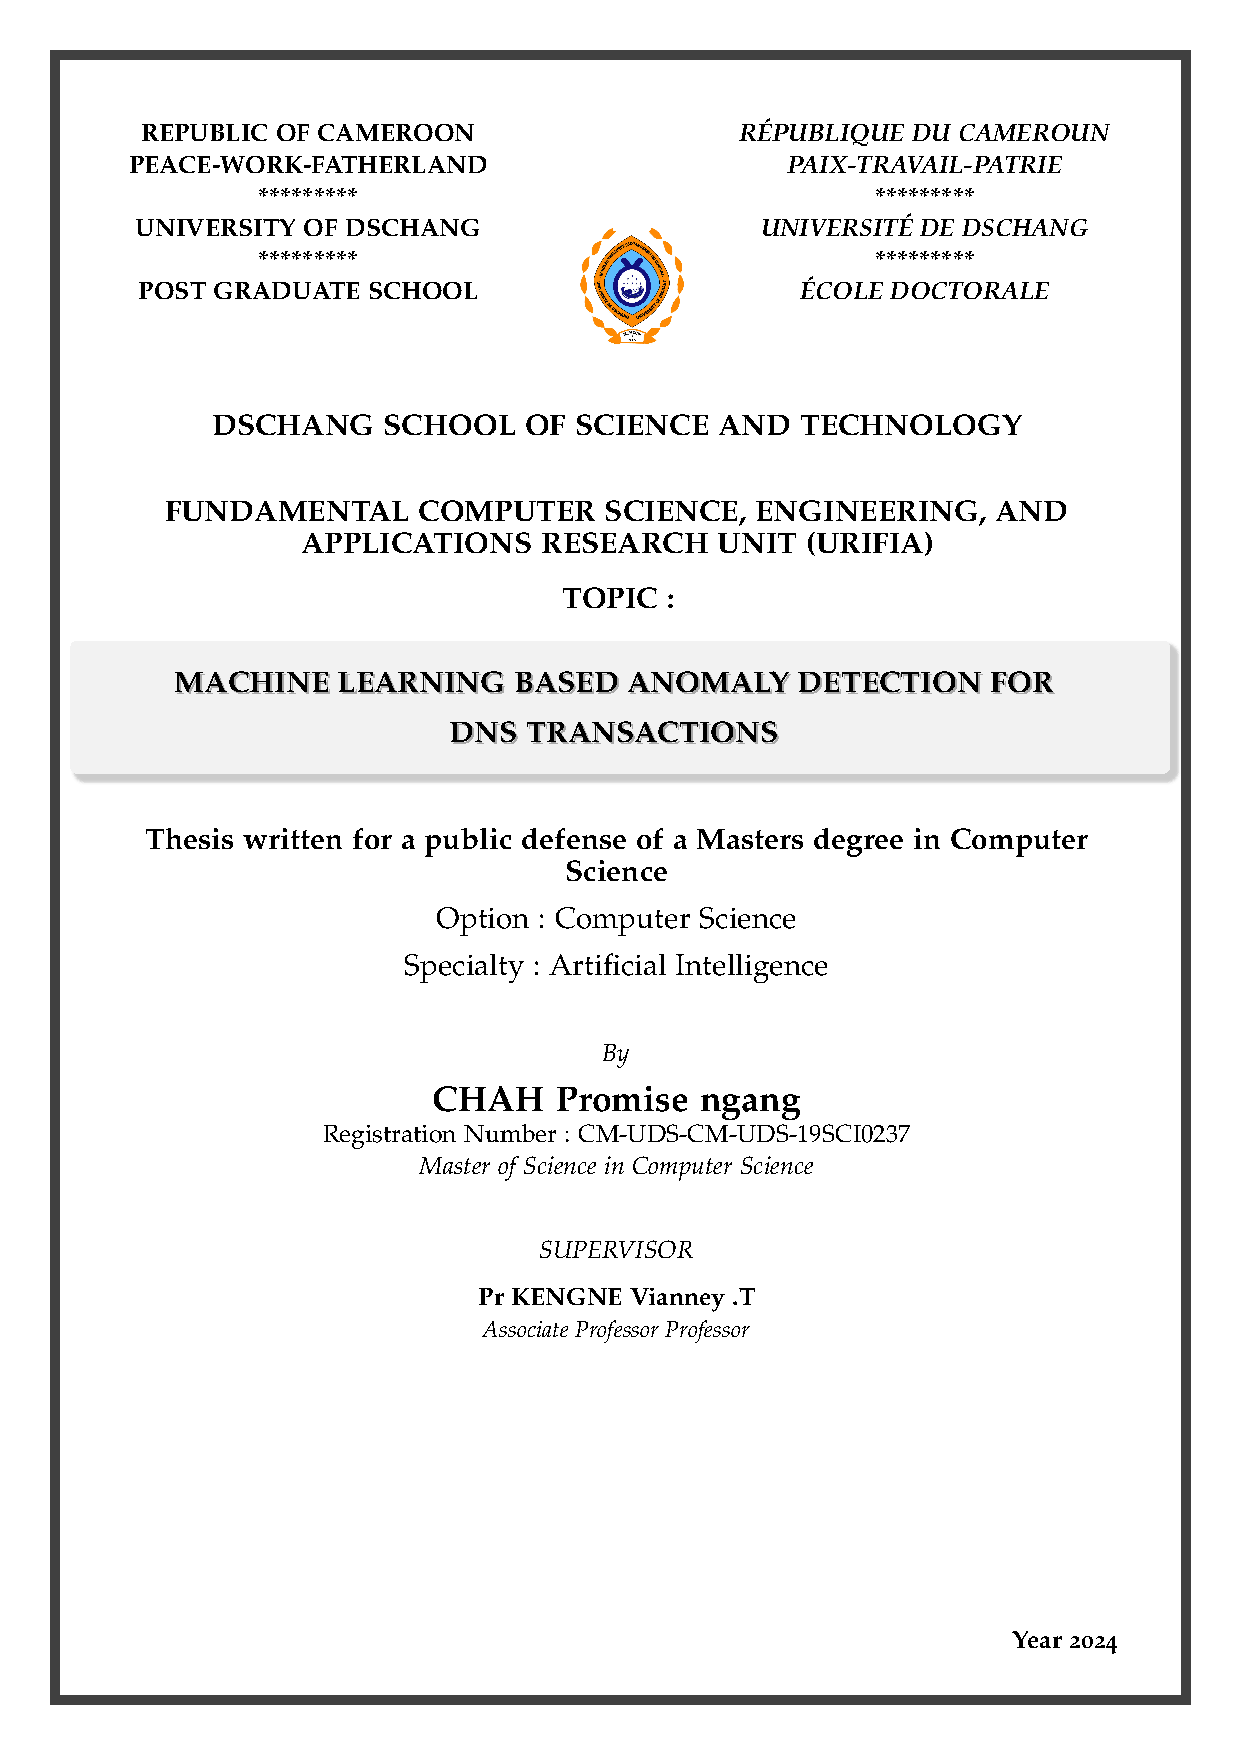
\includepdf[pages=-, offset=72 -72]{front-page1.pdf} %Insertion de la couverture
	%\includepdf[pages=-, offset=72 -72]{Originalite.pdf} %Attestation d'originalité
	%\includepdf[pages=-, offset=72 -72]{Correction.pdf} %Attestaion de correction

	\pagestyle{ruled}
	\nouppercaseheads
	\normalfont
	

	\frontmatter
	
	% Inclusion des fichiers de dédicaces et de remerciements
	%\myChapterStar{Titre}{Titre court}{Ajouter à la table des matières? (false|true|chapter|section|subsection|subsubsection -chapter par défaut-)}
\myChapterStar{Declaration of Authorship}{}{false}

        \begin{center}
            \textbf{CERTIFICATION }\\
        \end{center} 
                                            
                                            \vspace{1cm}   
I, the undersigned, CHAH Promise ngang, a student in Fundamental Computer Science, Registration Number CM-UDS-19SCI0237, option Artificial Intelligence, Department of Mathematics and Computer Science, Faculty of Sciences 
of the University of Dschang, certify that this dissertation entitled DNS abnomal attack detection using Machine Learning approach carried out at the Fundamental Computer Science, Engineering and Applications Research Unit (URIFIA) under the supervision of Pr Kengne vianney .T, associate Proffessor of the University of Dschang (Faculty of Sciences) is the fruit of my own research work. 
This dissertation is authentic and has never been presented for the award of any University Diploma or Degree.
\begin{center}
    

                        AUTHOR\\
                        \vspace{1cm}
                   CHAH Promise ngang\\
                                          \vspace{1cm}
                         SUPERVISOR\\
                                                \vspace{1cm}
                    Pr Kengne vianney .T\\

                            (Associate Professor) \\
                                            
                        HEAD OF DEPARTMENT\\
                                              \vspace{1cm} 
                    Pr NKENLIFACK Marcellin \\
                                           \vspace{1cm}
                                (Associate Professor)

\end{center}
	%\myChapterStar{Titre}{Titre court}{Ajouter à la table des matières? (false|true|chapter|section|subsection|subsubsection -chapter par défaut-)}
\myChapterStar{Dedications}{}{section}
\vspace*{7cm}
\begin{center}
\noindent \textit{\uppercase{TO} my father \textsc{CHAH JOHNSON TOYANG} and my mother \textsc{KAMDOUM ANNETTE CHANTAL}}.
\end{center}

\myCleanStarChapterEnd

	%\myChapterStar{Titre}{Titre court}{Ajouter à la table des matières? (false|true|chapter|section|subsection|subsubsection -chapter par défaut-)}
\myChapterStar{Acknowledgements}{}{section}
The achievements presented in this report would not be possible without God and the precious assistance of many people. Among these people I would like to particularly thank:
\begin{itemize} 

 \item  Pr KENGNE TCHENDJI Vianney and Mr Tangie yaweni my supervisor for their invaluable patience and feedback.They always supported and oriented me in the right direction. Their comments and suggestions were very helpful in the realization of this work;
 \item  The teaching staff of the Department of Mathematics and Computer Science.
They taught me the fundamentals which allowed me to increase my knowledge;
 \item  The jury members of this report for taking the time to give useful advice that
I gladly embrace for the improvement of this work;
 \item  My parents and siblings. I would be remiss in not mentioning my family
for the physical, emotional, moral and financial support whatever the circumstances. They were smart enough to remind me of my goals when I let myself
down in ease;
 \item  I also express my thanks to my academic elders for their precious advice and help;
 \item  I would like to express my sincere thanks to my classmates, particularly to Tiyo melong Rivaldes for the many exchanges we had in order to improve this work;
 \item Those whose name are not here and who contributed to this work.
\end{itemize}
\myCleanStarChapterEnd

	
	% Génération de la table des matières (avec "Table of Contents" comme titre), de la liste des symboles, de la liste des acronymes, de la liste des tableaux et de la liste des figures
	% Des alternatives à ces commandes sont dispos: il suffit juste d'ajouter le suffixe "Star" pour ne pas les mettre dans la table de matière
	\myTableOfContents{Table of Contents}
	\myListOfSymbols{}
	\myListOfAcronyms{}
	\myListOfTables{}
	\myListOfFigures{}
	
	% Resumé et abstract
	\let\oldprintchaptertitle=\printchaptertitle
\renewcommand{\printchaptertitle}[1]{%
	\vspace*{-75pt}
	\oldprintchaptertitle{#1}
}%
\myChapterStar{Résumé}{}{section}
\let\printchaptertitle=\oldprintchaptertitle
Dans le domaine de la cybersécurité, le système de noms de domaine (DNS) est crucial pour traduire les noms de domaine lisibles par l’homme en adresses IP, mais son rôle essentiel en fait également une cible fréquente des cyberattaques. Les modèles de classification binaire traditionnels, qui classent le trafic DNS comme « bénin » ou « malveillant », sont limités dans leur capacité à fournir des renseignements détaillés sur les menaces, nécessaires à une atténuation efficace des menaces. Ce travail vise à résoudre ces limitations en utilisant les techniques Ml pour transformer le problème de classification binaire en un problème de classification multi-classes, permettant ainsi une détection plus nuancée de divers types d'attaques basées sur le DNS.
Les principaux objectifs de cette recherche sont de prétraiter l'ensemble de données DNS, de mener une ingénierie approfondie des fonctionnalités grâce à une analyse de corrélation, d'appliquer des algorithmes d'apprentissage automatique (ML) tels que des algorithmes de clustering (DBSCAN) pour créer de nouvelles étiquettes de classe et de développer des modèles de classification multi-classes. Les modèles sont rigoureusement évalués à l’aide de mesures telles que l’exactitude, la précision, le rappel et le score F1. Ce modèle pourrait ensuite être déployé dans un environnement réel pour garantir son efficacité.
Nos contributions incluent l’amélioration de la granularité de la classification du trafic DNS, l’amélioration des processus d’ingénierie des fonctionnalités et l’avancement de la recherche sur la cybersécurité. En tirant parti de techniques de clustering avancées et en créant de nouvelles étiquettes de classe, notre approche fournit des renseignements détaillés sur les menaces, permettant ainsi des stratégies de réponse plus efficaces et ciblées. De plus, en mettant nos méthodologies et nos résultats à disposition sous forme de ressources open source, nous favorisons la collaboration et accélérons le développement de solutions de cybersécurité efficaces.
En conclusion, cette recherche transforme la classification binaire du trafic DNS en un problème de classification multi-classes, offrant des renseignements sur les menaces plus détaillés et plus exploitables. Cette approche globale améliore considérablement la détection et l'atténuation des attaques basées sur le DNS, renforçant ainsi la sécurité globale des systèmes réseau.

\vspace{1cm}
\noindent\textbf{Mots clés:} Cybersécurité, système de noms de domaine (DNS), trafic DNS, cyberattaques, classification binaire, classification multiclasse, apprentissage automatique (ML), ingénierie des fonctionnalités, analyse de corrélation, algorithmes de clustering DBSCAN, renseignement sur les menaces ; Exactitude, précision, rappel, score F1, attaques basées sur DNS Sécurité réseau.

\myCleanStarChapterEnd

	\myChapterStar{}{}{false}
\begin{center}
\chaptitlefont %\hrule height 1.5pt
\begin{center}\textcolor{black}{\textsc{Machine learning based anomaly detection for dns transactions}}
\end{center}
\end{center}
\vspace{8mm}
\textcolor{black}{\hrule height 4.5pt}%
\vspace{1mm}
\textcolor{black}{\hrule height 1.5pt}
	\let\oldprintchaptertitle=\printchaptertitle
\renewcommand{\printchaptertitle}[1]{%
	\vspace*{-75pt}
	\oldprintchaptertitle{#1}
}%
\myChapterStar{Abstract}{}{section}
\let\printchaptertitle=\oldprintchaptertitle


In the field of cybersecurity, the Domain Name System (DNS) is crucial for translating human-readable domain names into IP addresses, but its essential role also makes it a frequent target for cyberattacks. Traditional binary classification models, which categorize DNS traffic as either "benign" or "malicious," are limited in providing detailed threat intelligence necessary for effective threat mitigation. This work aims to address these limitations by using Ml technics to transform the binary classification problem into a multi-class classification problem, thereby enabling more nuanced detection of various types of DNS-based attacks.
The primary objectives of this research are to preprocess the DNS dataset, conduct thorough feature engineering through correlation analysis, apply machine learning(ML) algorithms like clustering algorithms(DBSCAN) to create new class labels, and develop multi-class classification models. The models are rigorously evaluated using metrics such as accuracy, precision, recall, and F1-score. This model could be then deployed in a real-world environment to ensure its effectiveness.
Our contributions include enhancing the granularity of DNS traffic classification, improving feature engineering processes, and advancing the state of cybersecurity research. By leveraging advanced clustering techniques and creating new class labels, our approach provides detailed threat intelligence, enabling more effective and targeted response strategies. Furthermore, by making our methodologies and findings available as open-source resources, we foster collaboration and accelerate the development of effective cybersecurity solutions.
In conclusion, this research transforms the binary classification of DNS traffic into a multi-class classification problem, offering more detailed and actionable threat intelligence. This comprehensive approach significantly improves the detection and mitigation of DNS-based attacks, ultimately enhancing the overall security of network systems.

\vspace{1cm}
\noindent\textbf{Keywords:} Cybersecurity, Domain Name System (DNS), DNS Traffic , Cyberattacks, Binary Classification, Multi-class Classification, Machine Learning (ML), Feature Engineering, Correlation Analysis, Clustering Algorithms DBSCAN ,Threat Intelligence; Accuracy, Precision, Recall, F1-score,DNS-based Attacks Network Security.
\myCleanStarChapterEnd

	\clearpage
	
	% *********** Partie principale ***********
	\mainmatter
	
	% Inclusion des différents chapitres
	%\myChapterStar{Titre}{Titre court}{Ajouter à la table des matières? (false|true|chapter|section|subsection|subsubsection -chapter par défaut-)}
\myChapterStar{General introduction}{}{true}
%\myMinitoc{Profondeur de la minitoc (section|subsection|subsubsection)}{Titre de la minitoc}
\myMiniToc{}{Contents}

%\mySectionStar{Titre}{Titre court}{Ajouter à la table des matières? (false|true|chapter|section|subsection|subsubsection -section par défaut-)}

\mySectionStar{Context of work}{}{true}
In the rapidly evolving landscape of cybersecurity, DNS (Domain Name System) plays a pivotal role as it is responsible for translating human-friendly domain names into IP addresses. This process is fundamental to the functioning of the internet. However, the ubiquity and criticality of DNS have also made it a frequent target for cyber-attacks. Attackers exploit DNS vulnerabilities to conduct a variety of malicious activities, including phishing, distributed denial-of-service (DDoS) attacks, and data exfiltration. As a result, monitoring and analyzing DNS traffic for signs of attack is essential for maintaining network security.
In this context, machine learning has emerged as a powerful tool for enhancing DNS security. By analyzing patterns in DNS traffic, machine learning models can effectively distinguish between benign and malicious activities. Traditionally, these models have focused on binary classification, categorizing traffic as either "attack" or "benign." However, the complexity of modern cyber threats demands a more nuanced approach. This work seeks to extend the capabilities of DNS traffic analysis by transforming a binary classification problem into a multi-class classification problem, thereby enabling more granular detection and response to different types of DNS-based attacks.
\mySectionStar{Problem statement}{}{true}
The core problem addressed in this work is the limitation of binary classification models in providing detailed threat intelligence from DNS traffic data. While these models can indicate whether traffic is benign or malicious, they do not offer insights into the specific type of attack. This lack of granularity can impede effective response and mitigation efforts, as different attacks may require different handling strategies.

To address this issue, this work proposes transforming the binary classification of DNS traffic into a multi-class classification problem. This involves not only detecting whether traffic is malicious but also identifying the specific type of attack. Achieving this requires a detailed analysis of DNS traffic features, the identification of relevant patterns and correlations, and the application of clustering techniques to uncover natural groupings within the data. These groupings can then be used to create new class labels, enhancing the classification model's ability to provide actionable insights.

\mySectionStar{Research hypothesis}{}{true}
The research hypothesis for this work is that transforming a binary DNS traffic
classification model into a multi-class classification model will significantly improve the granularity and utility of threat detection and response. Specifically, it
posits that by identifying and leveraging correlations between features within the
DNS dataset, it is possible to create new, meaningful classes that enhance the model’s ability to distinguish between different types of attacks. This, in turn, will
provide more detailed threat intelligence and improve the overall effectiveness of
cybersecurity measures.


\mySectionStar{ Objectives}{}{true}
 The general objective of this research is to develop an anomaly detection method for DNS transactions using multi-class classification and DBSCAN clustering to improve the precision,accuracy and reliability of detection compared to traditional binary classification. Specifically, the following are the specific objectives of this work:\\

\begin{itemize}
    \item Analyze the limitations of binary classification in DNS anomaly detection.

\item  Apply the DBSCAN clustering algorithm on the DNS transaction dataset to identify patterns and anomaly clusters.\\
\item Perform feature engineering based on clustering results to enrich the data and better characterize transactions.\\
\item Develop and train multi-class classification models to detect anomalies.\\
\item Compare the performance of multi-class models with binary models using appropriate metrics (precision, recall, F1-score).\\
\item Review the results against existing literature on DNS anomaly detection.
\end{itemize}
\mySectionStar{Our contribution}{}{true}
Our contributions lies on a good number of points which are listed below:
There are several works on DNS detection and classification going from traditional to
machine and deep learning techniques. As for machine learning techniques, we have
for example, Dharmaraj Patil et al.\cite{basnet2012learning} who proposed a binary phishing detection method using lexical and string complexity analysis of URLs, employing Confidence Weighted (CW) and Adaptive Regularization of Weight Vectors (AROW) classifiers to achieve high accuracy and efficiency. Again,Hanghang Liu et Haoran Zhang\cite{liu2020detecting}
proposed a method of detecting DNS tunelling traffic using binary classification model using SVM,RF and obtained high accuracy with SVM 99.66\%. On the other hand,M.Bakro et al \cite{moustafa2021building}Proposed a hybrid feature selection technic combining GOA and GA algorithm to proper select features in other to have proper informations about all features where they later applied their method on three rescent datasets to test the performance of their model. 
Our contribution include:\\
\begin{itemize}
    \item{Improving anomaly detection by proposing and architecture that intergrates DBSCAN clustering which reduces false positive and negative rates and improves classification accuracy on several dataset as compared to existing works. }\\
\end{itemize}
  \begin{itemize}
      \item{New insights for feature engineering are also promoted since DBSCAN clustering helps identify structures in the dataset that are not visible hence enriching feature engineering and data for more precise analysis.}
  \end{itemize}
    
\begin{itemize}
    \item{Methodological approach by combining clustering and multi-class classification offers a new methodology for anomaly detection in environments with limited feature information, applicable to other cybersecurity and data analysis fields.}
\end{itemize}
\begin{itemize}
    \item{Contribution to Literature by providing a detailed comparison between binary and multi-class approaches for DNS anomaly detection enriches existing literature and offers perspectives for future research in the field. Finally,establishing a correlation among fatures in the binary classification and optimizing hyparameters leading to a high performant model of accuracy 98.34\%}
\end{itemize}
\
\mySectionStar{Work outline}{}{true}
The rest of this document is organised as follows:\\
\textbf{Chapter I:Domain name system and machine learning:}In this chapter, we will
give an overview on DNS, its definition,how DNS works, types of DNS transactions (queries/responses) and servers. Then we will define ML, give a brief review of ML based techniques used in DNS security, some application of ML in cybersecurity. Finally, we will take the case of DNS.\\
\textbf{Chapter II:State Of the arts on anomaly detection in DNS transactions:}
In this chapter,
we will present DNS anomalies,starting from the traditional anomaliy techniques to Ml based techniques in binary and multi-class detection. Then we will present some supervised and unsupervised global ML approaches used in the literature to detect DNS anomalies. Finally, we will present some solutions present in the literature to face binary and multi-class anomaly detection in dns transactions as well as their advantages and disadvantages.\\
\textbf{Chapter III:Contribution to machine learning-based anomaly detection for DNS transactions:}
This chapter is dedicated to the presentation of our proposed solutions as well as their implementations. We start by describing our datasets for both binary and multi-class classification. Next, designing the model architecture and description of each component. Again,we will preprocess the data then select our model for training. Next, we will evaluate the results obtained after training based on performance metrics. Finally, we will compare the performance of both architectures together and with related works in a tabular form and discussions.\\
\textbf{Conclusion and future works:}
This section is the conclusion of our work which presents the overall functioning of our proposed models and approaches, as well as future works.
\myCleanStarChapterEnd

	%\myChapter{Titre}{Titre court}
\myChapter{Domain Name System and  Machine Learning}{}{}
%\myMinitoc{Profondeur de la minitoc (section|subsection|subsubsection)}{Titre de la minitoc}
\myMiniToc{}{Contents}

%\mySectionStar{Titre}{Titre court}{Ajouter à la table des matières? (false|true|chapter|section|subsection|subsubsection -section par défaut-)}
\mySection{Introduction}{}
The Domain Name System (DNS) is a hierarchical and decentralized naming system for devices connected to the internet or a private network. It translates human-friendly domain names like www.example.com into IP addresses like 192.0.2.1 that computers use to identify each other on the network. Without DNS, users would need to remember and use IP addresses to access websites or online services. In the other hand,artificial intelligence (AI) is the simulation of human intelligence processes by machines, especially computer systems. These processes include learning (the acquisition of information and rules for using the information), reasoning (using rules to reach approximate or definite conclusions), and self-correction. AI encompasses a variety of subfields and techniques aimed at enabling machines to perform tasks that typically require human intelligence. A major sub field of AI is Machine Learning (ML), which focuses on the development of algorithms that allow computers to learn from and make predictions based on data. Machine Learning is divided into several categories which ware going to be discussed later in this chapter.

\begin{figure}[ht!]
	\centering
	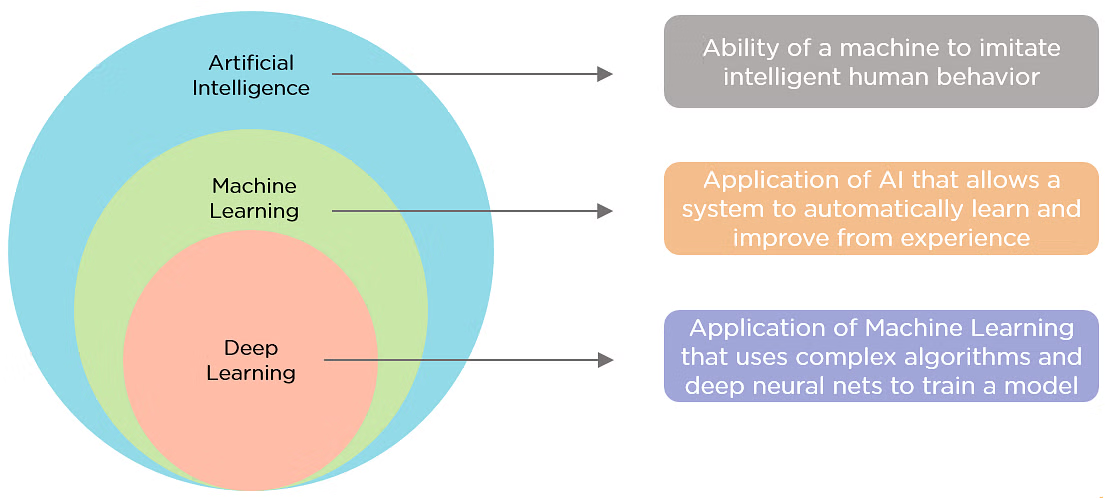
\includegraphics[width=0.9\linewidth]{Chap1/images/MLvsDLvsIA}
	\caption{The domains of {AI} \cite{shruti2023aivs}.}
	\label{fig:mlvsdlvsia}
\end{figure}
\mySection{Overview of DNS}{}
The Domain Name System (DNS) is an essential component of the internet infrastructure, functioning as the internet's directory. DNS translates human-friendly domain names like www.example.com into numerical IP addresses like 192.0.2.1 that computers use to identify each other on the network. This process is crucial because, while domain names are easy for people to remember, computers use IP addresses to locate and communicate with each other.

\subsection{Basic concepts}
\begin{enumerate}
	\item Domain Names:  A domain name is a string that identifies a realm of administrative autonomy, authority, or control on the internet. Examples include example.com, openai.com.
	
	\item IP Addresses: These are numerical labels assigned to each device connected to a computer network that uses the Internet Protocol for communication. They serve two main functions: identifying the host or network interface and providing the host's location.
\end{enumerate}
\subsection{DNS hierarchy:}
The DNS is organized in a hierarchical structure:

\begin{itemize}
	\item Root Level: The top of the DNS hierarchy, represented by a dot (.). It contains information that points to the top-level domain (TLD) servers.
	
	\item Top-Level Domains (TLDs): These are the highest level of domain names in the root zone. Common TLDs include .com, .org, .net, as well as country code TLDs like .uk, .jp.
	\item Second-Level Domains: These are directly below TLDs and are typically what people purchase from domain registrars (e.g., example in example.com).
	\item Subdomains: These are domains that are part of a larger domain (e.g., blog.example.com where blog is a subdomain of example.com).
\end{itemize}
\subsection{DNS-components}
\begin{itemize}
	\item DNS Resolvers: These are responsible for initiating and sequencing the queries that lead to a full resolution of the requested resource, usually managed by ISPs or enterprise networks.\\
	\item Root Name Servers: These servers know where to direct queries for each top-level domain (TLD).\\
	\item TLD Name Servers: These servers store information for each domain within the TLD and direct queries to the appropriate authoritative name servers.\\
	\item Authoritative Name Servers: These servers contain the actual DNS records for a domain and provide answers to queries about those records.
\end{itemize}
\subsection{DNS records:}
DNS records are used to store data about domain names. Key types include:\\

\begin{itemize}
	\item A Record: Maps a domain to an IPv4 address.\\
	\item AAAA Record: Maps a domain to an IPv6 address.\\
	
	\item CNAME Record: Canonical Name record; maps an alias domain name to the canonical domain name.\\
	\item MX Record: Mail Exchange record; specifies the mail server responsible for receiving email for the domain.\\
	\item NS Record: Name Server record; indicates which DNS server is authoritative for that domain.\\
	\item PTR Record: Pointer record; used for reverse DNS lookups to map an IP address to a domain name.\\
	\item TXT Record: Text record; used to store arbitrary text data, often for verification and security purposes.
\end{itemize}

\textbf{How DNS works\\}

Lets Consider the following figure:


\begin{comment}
	
	\begin{figure}[ht!]
		\centering
		\includegraphics[width=0.8\linewidth]{image dns good.png}
		\caption{How DNS resolution works \cite{cloudflare2023dns}}
		\label{fig:enter-label1}
	\end{figure}
\end{comment}

\begin{figure}[ht!]
	\centering
	\includegraphics[width=0.8\linewidth]{chap1/images/image dns good.png}
	\caption{how dns resolution works}
	\label{fig:enter-labeel1}
\end{figure}

\section*{How DNS Works}
Lets consider the workflow of DNS in  FIGURE \ref{fig:enter-label1} where a user enters a url through his or her web browser till when obtained the corresponding ip address. Lets explains detailly the scenario from ppoint 1 to 13: 
\begin{enumerate}
	\item \textbf{Query for the iP address:} When a user types a URL (e.g., http://mypage.com) into their web browser, the process of resolving the domain name to an IP address begins.
	
	\item \textbf{Local cache check:} The first step is to check if the IP address is stored in the local cache, which includes the browser cache, OS cache, and router cache. If the IP address is found here, the process stops, and the website is loaded from the cached IP address. If not, it moves to the next step.
	
	\item \textbf{Host files:} If the IP address is not found in the local cache, the system checks the host files. These files can manually map domain names to IP addresses. If the IP address is found in the host files, the process stops, and the website is loaded.
	
	\item \textbf{DNS resolver query:} If the IP address is not found in the local cache or host files, the query is sent to the DNS resolver, also known as a recursive resolver. This resolver is typically provided by the user's Internet Service Provider (ISP).
	
	\item \textbf{Root server query:} The DNS resolver then queries a root server. There are 13 sets of root servers worldwide, and they contain information on top-level domain (TLD) servers (such as .com, .org, .net).
	
	\item \textbf{TLD server query:} The root server responds with the address of a TLD server responsible for the queried domain. For example, if the query is for a .com domain, the root server provides the address of the .com TLD server.
	
	\item \textbf{Authoritative name server query:} The DNS resolver then queries the TLD server for the authoritative name server that holds the actual DNS records for the domain (mypage.com in this case).
	
	\item \textbf{Domain Nameserver Query:} The TLD server responds with the address of the domain's authoritative nameserver.
	
	\item \textbf{Authoritative nameserver response:} The DNS resolver queries the authoritative nameserver for the specific IP address of the domain (mypage.com).
	
	\item \textbf{IP address response:} The authoritative nameserver responds with the IP address of the requested domain.
	
	\item \textbf{Local cache update:} The DNS resolver stores the IP address in its local cache for future queries. This helps speed up the resolution process for subsequent requests for the same domain.
	
	\item \textbf{Query completion:} The DNS resolver sends the IP address back to the user's computer.
	
	\item \textbf{Website access:} With the IP address obtained, the user's computer can now contact the real server hosting the website (mypage.com) and load the webpage.
\end{enumerate}



\subsection{DNS anomalies}
Anomalies are patterns in data that deviate from the expected norm, arising from various abnormal activities such as credit card fraud, mobile phone fraud, and cyberattacks. These deviations are crucial for data analysts to identify. One important aspect of anomaly detection is understanding the nature of the anomaly, which can be categorized as follows:\\

\subsubsection{ Point anomaly}
When an individual data instance significantly deviates from the typical pattern of the dataset, it is identified as a point anomaly. For instance, if a person typically uses five liters of fuel per day for their car but suddenly uses fifty liters on a random day, this would be considered a point anomaly.

\subsubsection{ Contextual anomaly}
This type of anomaly occurs when a data instance is anomalous within a specific context, also known as a conditional anomaly. For example, credit card expenditures tend to be higher during festive periods such as Christmas or New Year. While high spending is normal for these contexts, it might be anomalous at other times of the year. Conversely, equally high expenditure during a non-festive month could be deemed a contextual anomaly.

\subsubsection{ Collective anomaly}
When a collection of similar data instances behaves anomalously with respect to the entire dataset, the group of data instances is termed a collective anomaly. For example, in a human's Electrocardiogram (ECG) output, the existence of low values for a long period of time indicates an outlying phenomenon corresponding to an abnormal premature contraction, whereas one low value by itself is not considered anomalous.
\subsubsection{ Seasonal anomaly}
Deviations from expected seasonal patterns. For instance, an unexpected spike in electricity consumption during a typically low-demand season could be a seasonal anomaly.

\subsubsection{ Spatial anomaly}
Anomalies that occur in a specific spatial context. For example, unusual traffic congestion in a normally low-traffic area could indicate a spatial anomaly.

\subsubsection{ Behavioral anomaly}
When an entity behaves differently than its usual pattern. For example, a user's sudden change in login times or locations could be considered a behavioral anomaly.
\subsection{DNS Attacks}
DNS attacks exploit vulnerabilities in the DNS protocol and infrastructure to disrupt normal operations or intercept data.

\subsubsection{Man-in-the-middle (MitM) attack}
\textbf{Overview\\}
In a MitM attack, the attacker secretly intercepts and relays messages between two parties who believe they are communicating directly with each other.\\

\begin{figure}[ht!]
	\centering
	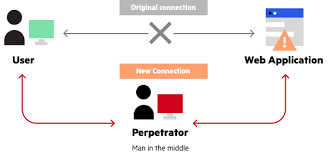
\includegraphics[width=0.5\linewidth]{chap1/images/man in the middle.png}
	\caption{Man in the middle attack \cite{howstuffworks2023dns}}
	\label{fig:enter-label}
\end{figure}


\textbf{How it Works}
\begin{enumerate}
	\item \textbf{Interception:} The attacker intercepts the communication channel between the client and the DNS server.
	\item \textbf{Relay:} The attacker can modify or eavesdrop on the messages.
	\item \textbf{Consequences:} This can lead to data theft, insertion of malicious content, or redirection to fake websites.
\end{enumerate}

\subsubsection{DNS Spoofing (DNS Cache Poisoning)}
\textbf{Overview\\}
DNS Spoofing, or DNS Cache Poisoning, involves corrupting a DNS server's cache with false information.


\begin{figure}[ht!]
	\centering
	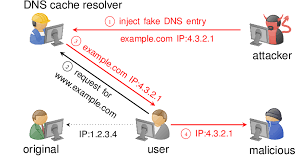
\includegraphics[width=0.5\linewidth]{chap1/images/cache poisning.png}
	\caption{Cache poisoning \cite{datadog2023dns}}
	\label{fig:enter-label}
\end{figure}


\textbf{How it Works}
\begin{enumerate}
	\item \textbf{Injection:} The attacker sends forged DNS responses to a DNS resolver.
	\item \textbf{Poisoning:} These false responses are cached by the DNS resolver.
	\item \textbf{Redirection:} Future queries for the poisoned domain are directed to the attacker's IP address.
	\item \textbf{Consequences:}
\end{enumerate}


Users can be redirected to malicious websites designed to steal information or infect devices with malware.

\subsubsection{DoS and DDos attacks}
A DoS attack aims to make a DNS server unavailable by overwhelming it with a large number of requests. In the other hand,a DDoS attack is a more powerful form of DoS, where multiple systems (often part of a botnet) are used to flood the DNS server with traffic.
\begin{figure}[ht!]
	\centering
	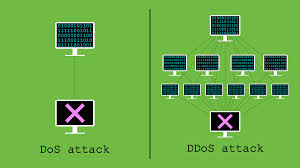
\includegraphics[width=0.5\linewidth]{chap1/images/dos.jpg}
	\caption{DoS and DDoS attack \cite{liquidweb2023dns}}
	\label{fig:enter-label}
\end{figure}

\textbf{How it Works}
\begin{enumerate}
	\item \textbf{Flooding:} The attacker sends a high volume of requests to the DNS server.
	\item \textbf{Overloading:} The server becomes overwhelmed and cannot process legitimate requests.
\end{enumerate}

\textbf{Consequences:}
Legitimate users are unable to resolve domain names, leading to service disruption.

\subsubsection{DNS Tunneling}

\textbf{Overview\\}
DNS Tunneling exploits DNS to tunnel malware and other data through a network firewall.

\begin{figure}[ht!]
	\centering
	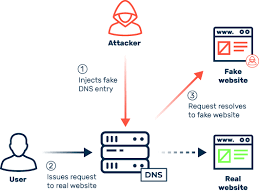
\includegraphics[width=0.5\linewidth]{chap1/images/dns spoofing.png}
	\caption{DNS tunneling \cite{cloudacademy2023dns}}
	\label{fig:enter-label}
\end{figure}

\textbf{How it Works}
\begin{enumerate}
	\item \textbf{Encoding Data:} Data is encoded into DNS queries.
	\item \textbf{Transmission:} These queries are sent to an external server controlled by the attacker.
	\item \textbf{Decoding Data:} The external server decodes the data from the DNS queries.
\end{enumerate}

\textbf{Consequences}
This technique can be used to exfiltrate sensitive information or establish command and control channels for malware.

\subsubsection{Cache Poisoning}
\textbf{Overview\\}
Cache poisoning is a specific type of DNS Spoofing that targets DNS caches, causing them to store incorrect information.

\begin{figure}[ht!]
	\centering
	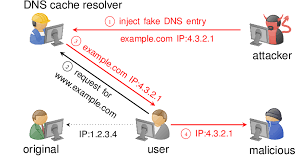
\includegraphics[width=0.5\linewidth]{chap1/images/cache poisning.png}
	\caption{cache poisonning\cite{datadog2023dns}}
	\label{fig:enter-label}
\end{figure}
\textbf{How it Works\\}
\begin{enumerate}
	\item \textbf{Forged Responses:} The attacker sends forged DNS responses to the DNS server.
	\item \textbf{Cache Storage:} These forged responses are stored in the DNS server's cache.
	\item \textbf{Misdirection:} Subsequent queries for the poisoned domain are directed to the attacker's IP address.
\end{enumerate}
\textbf{Consequences:}
Similar to DNS Spoofing, users are redirected to malicious sites, facilitating phishing, malware distribution, and other attacks.


\mySection{Types of Artificial Intelligence}{}

Artificial intelligence, so far, represents the ability of a program or a machine to solve complex problems by imitating human cognitive processes. It is also capable of performing intellectual tasks at a level often superior to humans in most cognitive domains. There are mainly two types of AI: strong artificial intelligence (AGI or strong AI) and weak artificial intelligence (weak AI).



\mySubSection{Weak Artificial Intelligence}{}

Weak AI, also called narrow AI, focuses on solving specific tasks, such as solving chess problems. Unlike general AI, this type of artificial intelligence does not exhibit creativity or the ability to learn autonomously in a universal way.\\ Its learning capabilities rely on pattern detection (machine learning) or comparing large amounts of data. The benefits of weak AI are particularly notable in automation and process control, as well as in speech recognition and processing. Among its applications are text and image recognition, speech recognition, text translation, and navigation systems, among others.
\mySubSection{Strong or General Artificial Intelligence}{}
General AI represents an artificial intelligence model designed to surpass human cognitive abilities in almost every field. Unlike weak AI, which is limited to specific tasks, general AI has the ability to analyze, interpret, and solve complex problems that arise in daily life. This includes advanced creativity skills, a deep and nuanced understanding of human emotions, and the ability to make autonomous decisions and move independently.
This form of AI could, for example, compose original music, write novels, or diagnose diseases with greater accuracy than the best human experts. It could also interact empathetically with humans, understand their emotional needs, and respond appropriately, while performing complex physical tasks without supervision \cite{elboudkhani2019}.
However, implementing general AI requires considerable investments in several areas. This includes massive financial resources for research and development, advanced computing infrastructures to manage large-scale data processing and storage, and a highly skilled workforce to design, program, and maintain these complex systems.

\begin{figure}[ht!]
    \centering
    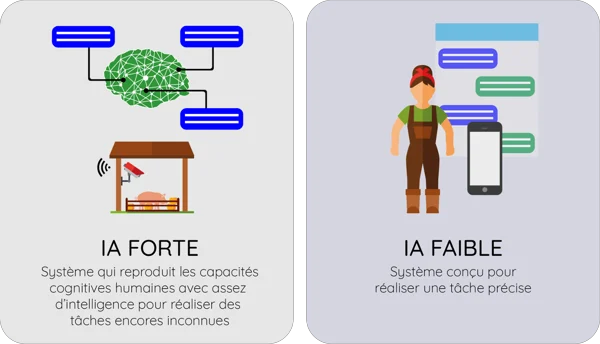
\includegraphics[width=0.8\linewidth]{chap1/images/IAFvsIAG.png}
    \caption{Weak AI vs.Strong AI}
    \label{fig:enter-label}
\end{figure}
\mySection{Machine Learning}{}

Machine Learning is an AI technology that aims to iteratively improve the performance of algorithms through data processing. In other words, Machine Learning allows computer systems to learn without being explicitly programmed for each task. Practically, this modern discipline allows for the discovery of patterns and predictions from data, relying on statistical methods, data mining, pattern recognition, and predictive analytics \cite{lebigdata2018}. Machine Learning is used in many fields such as speech recognition, fraud detection, consumer behavior prediction, and many more. Machine learning tasks are primarily organized into four categories: supervised learning, unsupervised learning, semi-supervised learning, and reinforcement learning.\\

\begin{figure}[ht!]
	\centering
	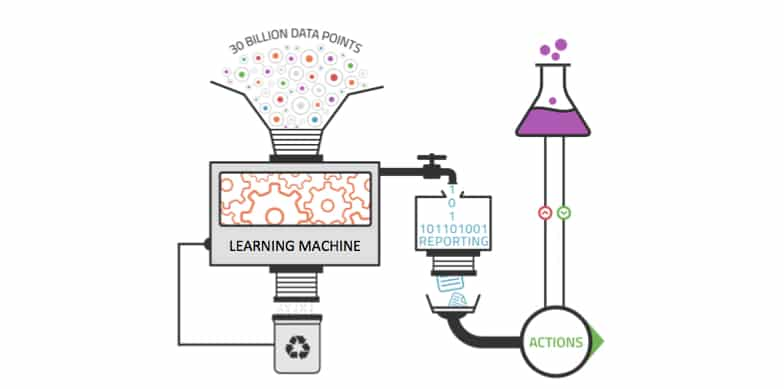
\includegraphics[width=0.8\linewidth]{Chap1/images/Marchinelearning2}
	\caption{Applications of Machine Learning \cite{lebigdata2018}.}
	\label{fig:marchinelearning2}
\end{figure}

\mySubSection{Supervised Learning}{}

Supervised learning is one of the most commonly used methods in the field of Machine Learning. It is a learning framework where an algorithm is trained on a labeled dataset. Each training example consists of an input and the corresponding output, allowing the algorithm to make predictions or classifications on new data based on the knowledge acquired during training, as shown in Figure \ref{MarchinelearningSupervise}. Supervised learning requires algorithms to train on a labeled dataset, and the goal is to map new input data to the desired target output value \cite{miraftabzadeh2019}.\\

\begin{figure}[ht!]
	\centering
	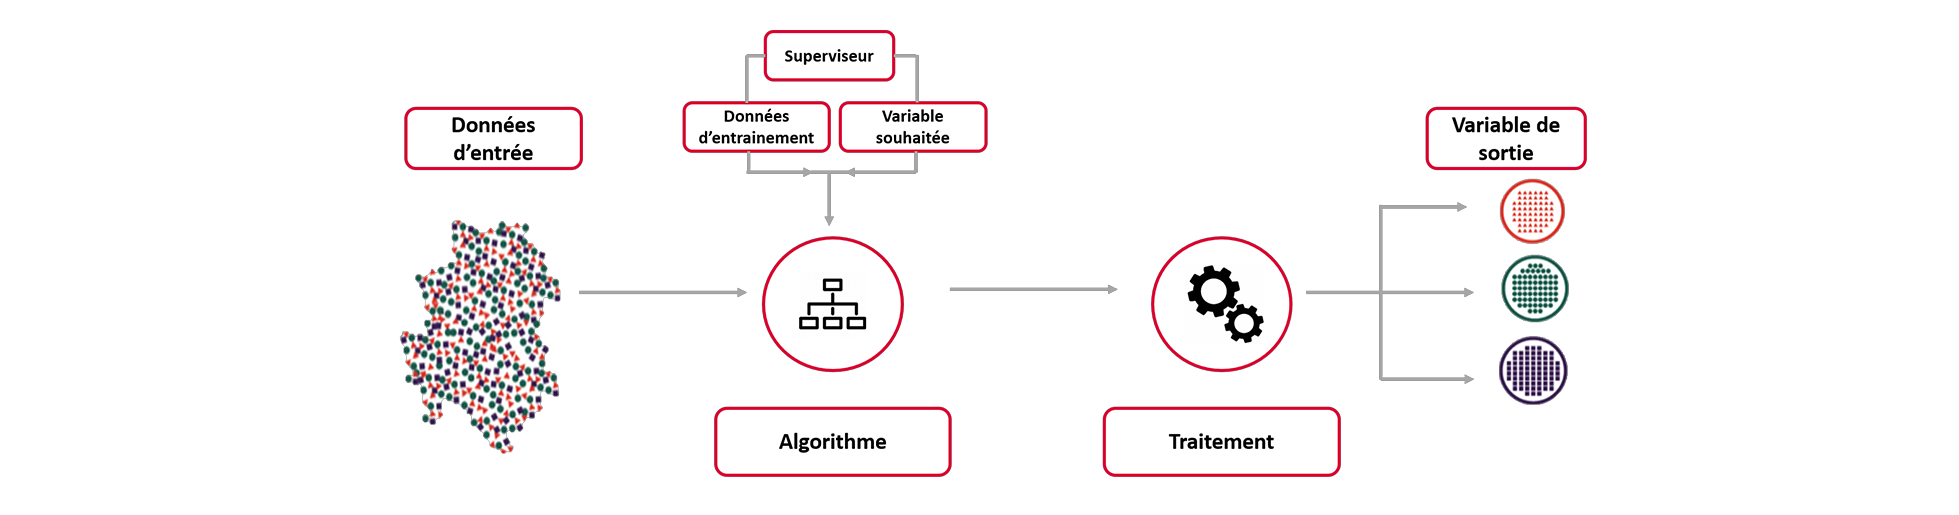
\includegraphics[scale=0.3]{Chap1/images/MarchinelearningSupervise}
	\caption{Supervised Learning \cite{Armandine2022}.}
	\label{MarchinelearningSupervise}
\end{figure}

Mathematically, problems in this type of learning are generally defined or formatted as follows: from a set of \( n \) observations \(\{\vec{x}1, \vec{x}_2, \ldots, \vec{x}_n\} = \{\vec{x}_i\}{i=1,\ldots,n}\) belonging to the set \(X\), and their labels \(\{y_1, y_2, \ldots, y_n\} = \{y_i\}_{i=1,\ldots,n}\) described in a set \(Y\), we aim to estimate the dependencies between the set \(X\) and \(Y\) to derive a model defined by a function \(y_i = f(\vec{x}_i) + \varepsilon_i\), where \(\varepsilon_i\) is a random noise. The algorithm, once trained with the provided labeled data, becomes capable of predicting labels on new unlabeled data.\\

\begin{figure}[ht!]
	\centering
	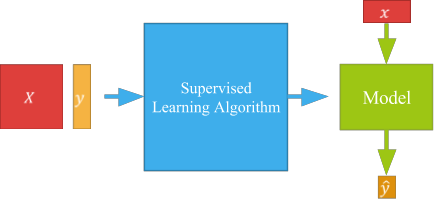
\includegraphics[scale=0.8]{Chap1/images/supervise.png}
	\caption{Supervised Learning}
	\label{fig:regressionvsclassification}
\end{figure}

In machine learning, the problems addressed are generally of two types: \textbf{Regression problems} and \textbf{Classification problems}.
\begin{enumerate}
	\item \textbf{Regression Problems:} These involve predicting continuous or real values based on input variables.
	\item \textbf{Classification Problems:} This involves predicting a discrete output variable, often called class labels, from a set of input data.
\end{enumerate}

\begin{figure}[ht!]
    \centering
    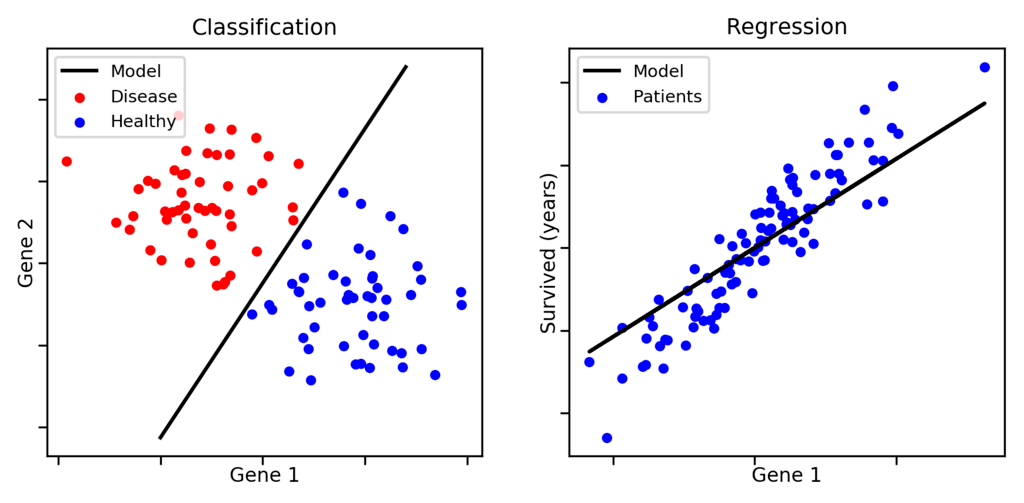
\includegraphics[width=0.6\linewidth]{chap1/images/regressionVSclassification.png}
    \caption{regression Vs.classification\cite{tensorflow2023}}
    \label{fig:enter-label}
\end{figure}

Over time, several algorithms have been developed to address the various problems of supervised learning. Among the main ones are:

\begin{itemize}
	\item \textbf{Linear Regression:} Used to predict the value of a dependent variable based on an independent variable . For example, predicting annual sales based on the education level or experience of a salesperson.

\begin{figure}[ht!]
    \centering
    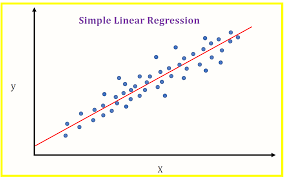
\includegraphics[width=0.5\linewidth]{chap1/images/linear regression.png}
    \caption{linear regression\cite{scikit-learn2023}}
    \label{fig:enter-label}
\end{figure}

 
	\item \textbf{Logistic Regression:} Suitable when dependent variables are binary.{SVM} is a relevant alternative when dependent variables are more difficult to classify.

    
 
	\item \textbf{Decision Trees:} Allow recommendations based on decision rules derived from classified data. For example, recommending a football team to bet on based on data like players' ages or the team's win percentage.






\item \textbf{Random Forest:} A collection of decision trees, where each tree is based on a bootstrap sample \cite{ho1998random}. The judgment is obtained by majority vote (classification) or by averaging results (regression).


 \begin{figure}[ht!]
     \centering
     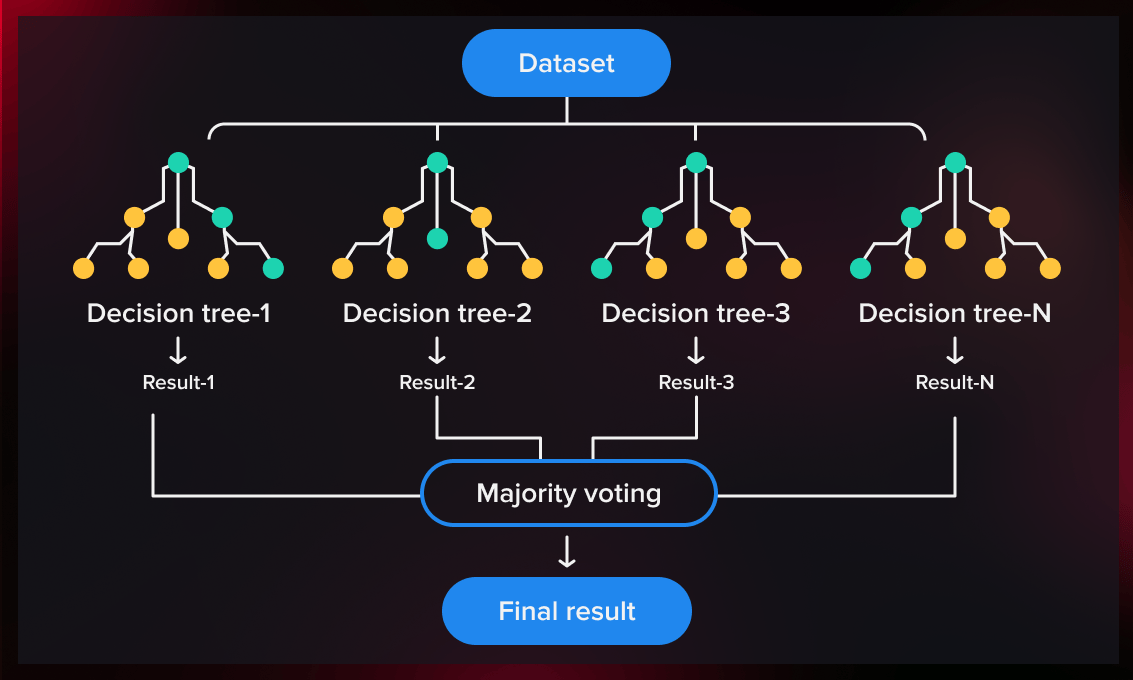
\includegraphics[width=0.5\linewidth]{chap1/images/randomforest.png}
     \caption{random forest\cite{ho1998random}}
     \label{fig:enter-label}
 \end{figure}

 
	\item \textbf{{SVM}:} Used for classification or regression. It uses a technique called the kernel trick to transform data and find an optimal boundary between possible outputs \cite{cortes1995support}.



 
	\item \textbf{Neural Networks:} Generally performed using a computer, reproducing or predicting the behavior of processes based on the factors that determine them.


 \begin{figure}[ht!]
     \centering
     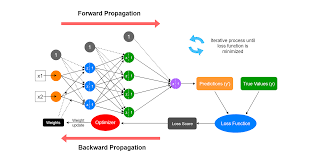
\includegraphics[width=0.5\linewidth]{chap1/images/neural network.png}
     \caption{neural network\cite{neuralnetwork2023}}
     \label{fig:enter-label}
 \end{figure}
	\item \textbf{{KNN}:} A classification algorithm that uses the similarity of neighboring data points to predict the class label of a new sample.


 \begin{figure}[ht!]
     \centering
     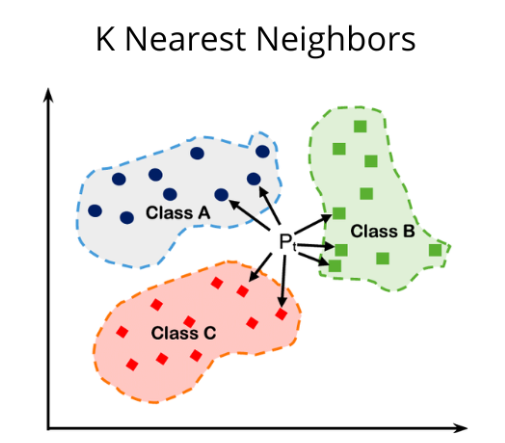
\includegraphics[width=0.5\linewidth]{chap1/images/knn.png}
     \caption{knn\cite{knn2023}}
     \label{fig:enter-label}
 \end{figure}
\end{itemize}

\mySubSection{Unsupervised Learning}{}

Unsupervised learning explores data without corresponding output variables, allowing it to discover the underlying structure or distribution of the data. Unlike supervised learning, where algorithms are guided by correct answers, unsupervised learning operates autonomously, seeking to identify patterns and intrinsic structures in the data \cite{ismaili2019}. The two main categories of algorithms in unsupervised learning are clustering and association. Clustering aims to divide a dataset into homogeneous groups, while association seeks to discover interesting relationships between variables in large databases.

\begin{figure}[ht!]
	\centering
	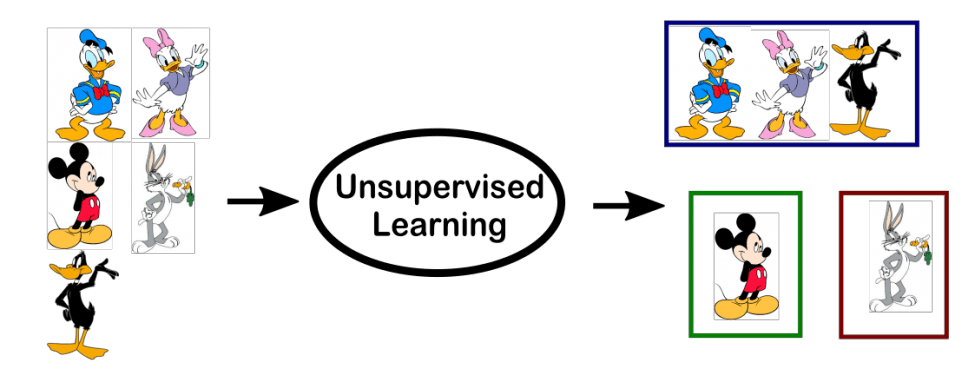
\includegraphics[scale=0.6]{Chap1/images/regressionVSclassification2}
	\caption{Unsupervised Learning \cite{ismaili2019}}
	\label{fig:regressionVSclassification2}
\end{figure}

In this subfield, several algorithms are commonly used:
\begin{itemize}
	\item \textbf{K-means Clustering:} It is an unsupervised learning algorithm used to solve clustering problems. K-means groups similar data points into clusters based on their characteristics or similarities \cite{pelleg1999accelerating}.
	\item \textbf{Association Rules:} These algorithms identify frequent relationships and associations between variables in datasets \cite{kamsu2013mining}.
	\item \textbf{Dimensionality Reduction:} This technique reduces the number of variables or features in a dataset while preserving relevant information. PCA is one of the popular methods for dimensionality reduction \cite{pelleg1999accelerating}.
\end{itemize}

\mySubSection{Semi-supervised Learning}{}

In machine learning, problems involving a large amount of input data (X = \(\{\vec{x}_1, \vec{x}_2, \ldots, \vec{x}_n\}\)) with only a few labeled data (Y = \(\{\vec{y}_1, \vec{y}_2, \ldots, \vec{y}_n\}\)) are called semi-supervised learning problems \cite{ismaili2019}. These problems lie between supervised learning, where all data is labeled, and unsupervised learning, where no labels are available.
A concrete example of a semi-supervised problem would be an archive of photos where only a few images are labeled (e.g., dog, cat, person) while most are not. In many real cases, labeling all data can be time-consuming or expensive, often requiring the expertise of domain specialists. Consequently, unlabeled data are often easier to collect and store.
To address semi-supervised problems, various techniques can be used. For example, unsupervised learning methods can be applied to discover and learn the underlying structure of input variables \cite{song2014semi}.
\mySubSection{Reinforcement Learning}{}
Reinforcement learning is a form of machine learning that focuses on training an algorithm to make decisions based on the rewards and punishments it receives. Unlike other methods where input-output pairs are provided, in reinforcement learning, we describe the current state of the system, specify a goal, provide a list of allowed actions with their environmental constraints, and then let the machine learning model experiment with achieving the goal on its own. This model uses the trial-and-error principle to maximize a reward \cite{zschech2021machine}.

\begin{figure}[ht!]
	\centering
	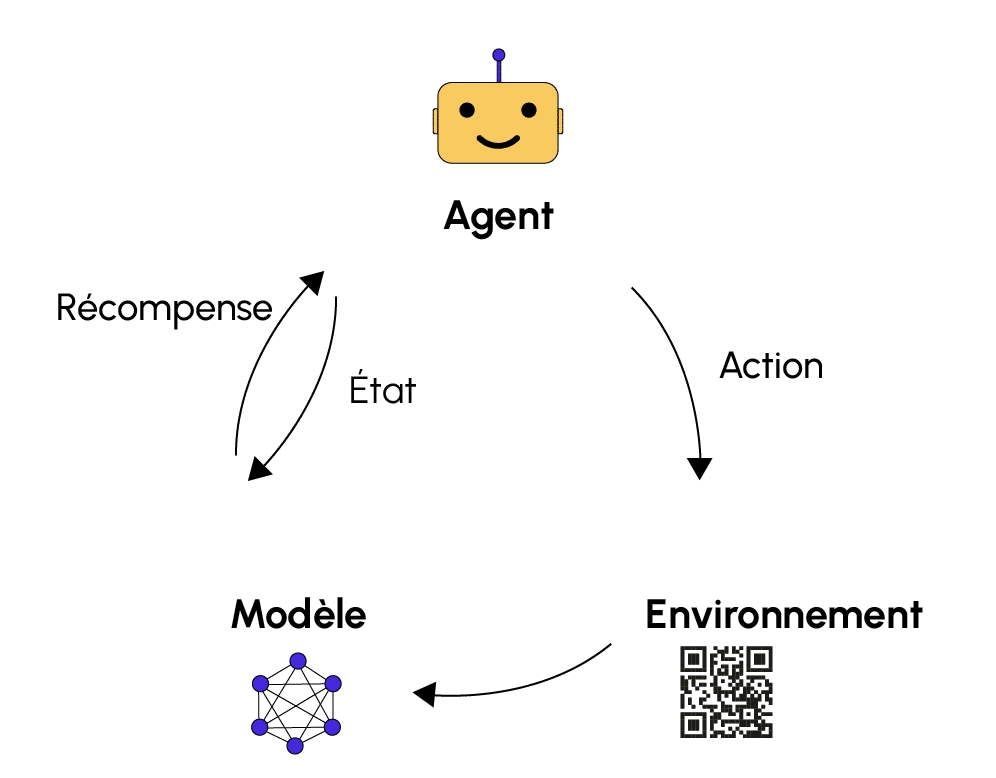
\includegraphics[scale=0.6]{Chap1/images/renforcement3}
	\caption{Reinforcement learning \cite{ismaili2019}}
	\label{fig:renforcement3}
\end{figure}

Reinforcement learning, as illustrated in Figure \ref{fig:renforcement3}, involves the use of several essential concepts and metrics, among which the main ones are as follows:

\begin{itemize}
	\item \textbf{Agent}: a system or robot that interacts and acts in the environment.
	\item \textbf{Action \( a \)}: an action selected from the set of possible actions.
	\item \textbf{State \( s \)}: a particular situation in which the agent finds itself.
	\item \textbf{Reward \( r(s,a) \)}: a positive or negative gain obtained by performing action \( a \) in state \( s \). The goal is to maximize the total benefits of a policy.
\end{itemize}


\mySection{Data Mining}{}
With the advent of artificial intelligence, the value of data has become crucial. Their diversity and rapid accumulation have resulted in an impressive mass of data requiring thorough analysis to be fully utilized. In this context, the implementation of analysis tools capable of extracting relevant information from these data is of paramount importance for data analysis professionals. For several decades, data mining has been the preferred method. This approach aims to search for and extract useful and unknown information from large sets of data stored in databases or data warehouses. The emergence of data mining in the 1990s was facilitated by technological advances that improved the computing power of computers. Data mining tools offer powerful statistical, mathematical, and analytical capabilities, aiming to analyze large datasets to identify trends, patterns, and relationships, to make informed decisions and plan effectively.

\mySubSection{Data Mining Process and Operation}{}

Data mining is generally carried out by data scientists and other professionals specializing in data analysis. However, it can also be undertaken by business analysts and personnel with a solid understanding of data, acting as data scientists within the organization. The essential elements of this exploration include machine learning, statistical analysis, as well as data management tasks necessary to prepare the data for analysis. The use of artificial intelligence (AI) tools has automated much of this process and simplified the exploration of massive datasets, such as customer databases or transaction records. The data mining process can be broken down into five steps, as illustrated in the following figure (Figure \ref{fig:datami}).

\begin{figure}[ht!]
	\centering
	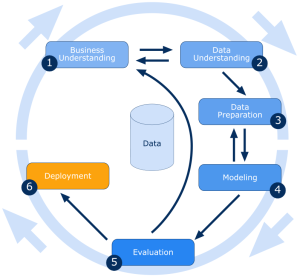
\includegraphics[scale=0.9]{Chap1/images/DataMi1}
	\caption{Data Mining Process \cite{kumar2023different}}
	\label{fig:datami}
\end{figure}

\begin{enumerate}
	\item \textbf{Understanding the Problem:} Before any data is touched, extracted, cleaned, or analyzed, it is important to understand the underlying entity and the ongoing project. It is also crucial to define the objectives to be achieved for problem resolution.
	
	\item \textbf{Data Collection:} This phase involves collecting the data that will be subjected to analysis. These data may be located in various source systems, such as data warehouses, which are increasingly used in big data environments. Data are also gathered from multiple external sources. These storage locations contain a mix of structured data (e.g., database tables) and unstructured data (e.g., text documents, images, videos). Regardless of the origin of the data, a data scientist often moves them to a data warehouse for subsequent process steps.
	
	\item \textbf{Data Preparation:} This phase is one of the most crucial phases of the process. It involves performing a set of treatments on the data to make them usable. It begins with data exploration, profiling, and preprocessing, followed by data cleaning to correct errors and other data quality issues. These issues include duplicates in the data, inconsistencies, incomplete records, or obsolete formats.
	
	\item \textbf{Modeling:} After the data preparation phase comes the information extraction phase. This step involves selecting the appropriate data mining technique and implementing one or more algorithms to perform the mining. These algorithms are machine learning algorithms that will train on these data to make the prediction process faster.
	
	\item \textbf{Evaluation:} Once the information extraction models' training is complete, the performance of the data models is evaluated. The analysis results can be aggregated, interpreted, and presented to decision-makers who have been largely excluded from the data mining process until now. At this stage, organizations can choose to make decisions based on the results.
\end{enumerate}

\mySubSection{Data Mining Techniques}{}

Data mining uses a set of algorithms and various techniques to convert large volumes of data into useful information. Here are some of the most popular techniques:

\begin{itemize}
	\item \textbf{Association Rules:} This technique aims to discover patterns in the data. Association rules, in the form of "if...then" statements, identify relationships between data items. Support measures how frequently these relationships appear, while confidence evaluates their accuracy. Popular algorithms include Apriori and FP-Growth.
	
	\item \textbf{Clustering:} Used in the absence of information about the types of data objects, clustering aims to group similar data. Common algorithms include K-means and hierarchical classification.
	
	\item \textbf{Classification:} To classify data into different groups based on a target attribute, classifiers predict the target label for each record. Common techniques include decision trees, neural networks, k-nearest neighbors (K-Means), support vector machines (SVM), and Bayesian methods.
	
	\item \textbf{Regression:} To model the relationships between variables and predict continuous numerical values, regression uses algorithms such as linear regression, logistic regression, and polynomial regression.
\end{itemize}

These techniques are essential for extracting meaningful information from data and making informed decisions in many fields.

\mySubSection{Importance of Data Mining}{}

Data mining is an essential process in data science that enables engineers to better understand their datasets. This process is of crucial importance in data analysis across various fields for the following reasons:

\begin{itemize}
	\item \textbf{Decision Making from Large Amounts of Data:} Data mining allows for extracting knowledge and hidden patterns from data. It helps organizations make informed decisions based on factual information rather than assumptions or intuitions. This can lead to more effective and profitable decisions.
	
	\item \textbf{Detection of Patterns and Trends:} Data mining helps discover significant patterns, correlations, and trends in the data. These insights can help organizations identify opportunities, anticipate future behaviors, detect market changes, and take preventive or proactive measures.
	
	\item \textbf{Forecasting and Planning:} By analyzing historical data and identifying relationships between variables, data mining can be used to predict future outcomes and establish plans and strategies accordingly. This can be useful in inventory management, demand forecasting, financial planning, etc.
	
	\item \textbf{Segmentation and Targeting:} Data mining allows grouping individuals or objects based on their common characteristics. This enables organizations to better understand their customers, segment the market into homogeneous groups, tailor offers and marketing campaigns accordingly, and target advertisements more precisely.
	
	\item \textbf{Personalization and Recommendation:} Data mining helps build personalized recommendation systems by analyzing users' preferences, behaviors, and purchase histories. This enhances user experience by providing relevant recommendations and increasing conversion and retention rates.
\end{itemize}

\mySubSection{Applications of Data Mining}{}

Data mining can be applied to all sectors that generate data and wish to benefit from it. Indeed, access to data is the key element to answering several questions within a domain. Here are some examples of how data mining is used in specific industries:

\begin{itemize}
	\item \textbf{Healthcare:} For many years, the integration of data mining in healthcare has enabled doctors to benefit from more effective treatment methods using data extracted from clinical trials and patient studies. Hospitals and clinics can thus improve patient outcomes and safety while reducing costs and response times.
	
	\item \textbf{Media and Telecommunications:} Companies in the media and telecommunications sector have access to an enormous amount of data on consumer preferences, such as the shows they watch or the internet plans they subscribe to. With these data, these companies can tailor their programming to consumer tastes, region, or other relevant factors. They can even recommend content to consume, a practice mastered by companies like Orange Cameroon, MTN Cameroon, YouTube, etc.
	
	\item \textbf{Bioinformatics:} Data mining plays an important role in the field of bioinformatics. Indeed, it is used to extract and analyze information on sequences, molecules, and gene expression to understand the functioning of certain biological processes.
\end{itemize}
\mySection{Conclusion}{}
In this chapter, we explored the interaction between the Domain Name System (DNS) and Machine Learning (ML), highlighting how ML enhances DNS security and performance. DNS, essential for translating domain names into IP addresses, is vulnerable to various attacks. ML offers powerful tools to detect and mitigate these threats by analyzing patterns and predicting anomalies.Key benefits of integrating ML with DNS include improved threat detection, anomaly identification, predictive analytics, and operational efficiency. However, challenges such as data privacy and model interpretability must be addressed. Finally,combining ML with DNS significantly enhances cybersecurity, ensuring a more secure and reliable internet infrastructure. Continued research and development in this field promise to refine these techniques and further strengthen DNS security.













































\begin{comment}
\mySection{Machine learning-based techniques}{}

Machine learning is a branch of Artificial Intelligence (AI) that empowers systems to learn and improve automatically from experience without needing explicit programming. The focus of machine learning is on developing computer programs that can access data and learn autonomously.Machine learning can be divided into three primary categories: supervised learning, unsupervised learning, and reinforcement learning.\\




\begin{figure}[ht!]
    \centering
    \includegraphics[width=0.75\linewidth]{Capture d'écran 2024-06-11 131107.png}
    \caption{Relatioship between Artificial intelligence,Machine learning and Deep learning}
    \label{fig:enter-label}
\end{figure}






\subsection{Supervised machine learning}

Supervised machine learning involves training algorithms to make predictions or classify data based on labeled training data. In supervised learning, the algorithm is trained on a dataset with known outcomes, allowing it to generalize from the labeled examples to make predictions on new, unseen data.The fundamental components in supervised machine learning are:
\begin{itemize}
    \item \textbf{Input (X)}: The data used by the model to make predictions.
    \item \textbf{Output (Y)}: The correct label or outcome for each example in the training data.
    \item \textbf{Output (f)}: The function that the algorithm learns to map inputs to outputs. The goal is to find the best model that accurately predicts the correct output for new input data.
\end{itemize}
The general equation for a supervised learning model is:
\[ Y = f(X) + \text{error} \]
where "error" signifies the difference between the predicted and actual outputs.
This type of learning is termed supervised because the algorithm's learning process from the training dataset is akin to a teacher supervising the process. The algorithm iteratively makes predictions on the training data and is corrected by the teacher until it reaches an acceptable performance level. Supervised learning algorithms are further categorized into regression and classification algorithms.

\textbf{Classification}: Tasks where the goal is to predict a categorical outcome, such as whether an email is spam. Common algorithms include logistic regression, decision trees, and support vector machines.

\textbf{Regression}: Tasks where the goal is to predict a continuous outcome, such as house prices. Common algorithms include linear regression, decision trees, and neural networks.

Some common supervised learning algorithms include:
\begin{itemize}
    \item \textbf{Support Vector Machines (SVM)}: Used for both classification and regression tasks, finding the hyperplane that best separates the data into classes or predicts values.






    \begin{figure}[ht!]
        \centering
        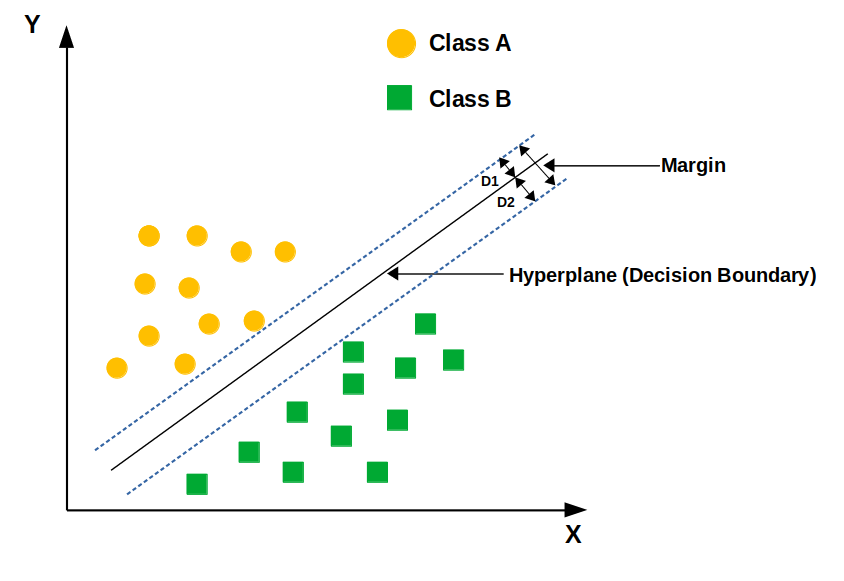
\includegraphics[width=0.5\linewidth]{svm.png}
        \caption{SVM}
        \label{FIGURE 2}
    \end{figure}


    
    \item \textbf{Neural Networks}: Used for diverse tasks like image recognition and speech recognition, consisting of interconnected nodes that learn from input data.



    \begin{figure}[ht!]
        \centering
        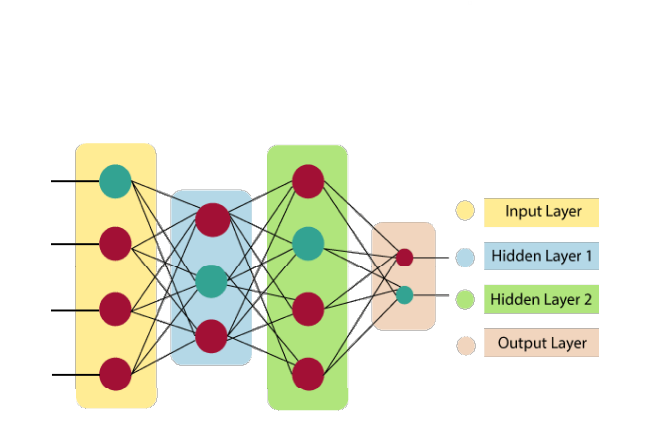
\includegraphics[width=0.5\linewidth]{rnn.png}
        \caption{Neural network}
    \end{figure}


    
    \item \textbf{Linear Regression}: Used for regression tasks, modeling the relationship between input and output variables using a linear function.

    \item \textbf{Logistic Regression}: Used for binary classification tasks, modeling the probability of outcomes using a logistic function.

\begin{figure}[ht!]
    \centering
    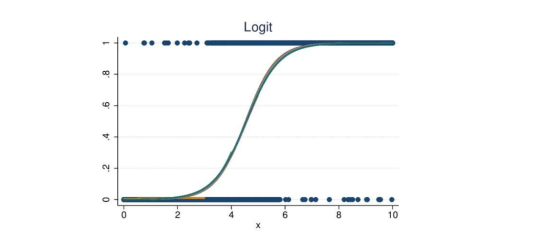
\includegraphics[width=0.5\linewidth]{logistic regrestion.png}
    \caption{logistic regression}
    \label{fig:enter-label}
\end{figure}


    
    \item \textbf{Decision Trees}: Used for both classification and regression tasks, creating a tree-like model of decisions.



    

\begin{figure}[ht!]
    \centering
    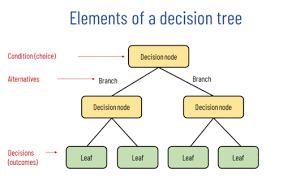
\includegraphics[width=0.3\linewidth]{decision tree.png}
    \caption{Decision tree}
    \label{fig:enter-label}
\end{figure}



    
    \item \textbf{Random Forest}: An extension of decision trees, combining multiple trees to improve accuracy and reduce over-fitting.
    \item \textbf{K-Nearest Neighbors (KNN)}: Used for classification, classifying new data points based on the K nearest neighbors in the training set.
\end{itemize}

\subsection{Unsupervised Machine Learning}

Unsupervised machine learning involves algorithms learning from unlabeled data. Unlike supervised learning, there is no target variable, and the algorithm seeks to find patterns and relationships in the data without predefined outputs. Unsupervised learning is useful for exploratory data analysis, detecting anomalies, clustering similar data points, and reducing data dimensionality.\\

Types of unsupervised learning algorithms include:
\begin{itemize}
    \item \textbf{Clustering}: Grouping similar data points based on feature similarity.
    \item \textbf{Dimensionality Reduction}: Reducing the number of features while preserving important information to simplify data analysis.
    \item \textbf{Association Rule Learning}: Finding relationships between variables in the data, identifying frequent co-occurrences of items.
\end{itemize}

Common unsupervised learning algorithms include:
\begin{itemize}
    \item \textbf{K-Means Algorithm}: Used for clustering.
    \item \textbf{Principal Component Analysis (PCA)}: Used for dimensionality reduction.
    \item \textbf{A priori Algorithm}: Used for association rule learning.
\end{itemize}

\subsection{Reinforcement Learning}

Reinforcement learning involves an agent learning to make decisions by interacting with an environment. The agent receives feedback as rewards or punishments based on its actions and learns to optimize its behavior to maximize rewards. Reinforcement learning is used in applications such as robotics, game playing, and autonomous vehicles.
At a high level, reinforcement learning can be formulated as a Markov decision process (MDP) consisting of:
\begin{itemize}
    \item \textbf{Environment}: The physical world in which the agent operates.
    \item \textbf{State}: The current situation of the agent.
    \item \textbf{Reward}: Feedback from the environment.
    \item \textbf{Policy}: The method to map an agent's state to actions.
    \item \textbf{Value}: The future reward an agent would receive by taking an action in a particular state.
\end{itemize}

\subsection{Federated Learning}

Federated learning is a decentralized machine learning approach that enables multiple parties to collaboratively train a model without sharing their data. Training data remains on the participants' devices, with only model updates being exchanged. This approach preserves data privacy and reduces communication costs.\\

Types of federated learning include:
\begin{itemize}
    \item \textbf{Horizontal Federated Learning}: Participants have the same features but different samples.
    \item \textbf{Vertical Federated Learning}: Participants have different features but the same samples.
\end{itemize}

\subsection{Deep Learning}

Deep learning, a subset of machine learning, involves training artificial neural networks with multiple layers to perform complex tasks such as image recognition, speech recognition, natural language processing, and autonomous driving. Unlike traditional machine learning algorithms that require manual feature engineering, deep learning algorithms can automatically learn high-level features from raw data, making them effective for tasks where relevant features are not well understood.

Neural networks consist of layers of interconnected nodes, called neurons, performing simple calculations on input data. The output of one layer serves as input to the next layer, allowing the network to learn increasingly complex data representations.
\mySection{Machine learning in DNS security}{}
DNS (Domain Name System) is a critical component of the internet infrastructure, responsible for translating human-readable domain names into IP addresses. As the internet continues to grow, DNS has become an increasingly attractive target for cyber attackers, who may attempt to exploit vulnerabilities in the system to launch various types of attacks, such as domain name hijacking, cache poisoning, and distributed denial-of-service (DDoS) attacks. ML has emerged as a powerful tool in the field of DNS security, enabling the detection and mitigation of these threats. ML algorithms can analyze large volumes of DNS traffic data, identify patterns and anomalies, and quickly detect and respond to potential attacks. This can greatly improve the overall security and reliability of the DNS system, protecting both individuals and organizations from the consequences of DNS-based attacks.
\subsection{Application of ML in cybersecurity}
In the rapidly evolving landscape of cybersecurity, the advent of machine learning (ML) has brought about a transformative shift in the way we approach the detection, prevention, and mitigation of cyber threats. As the volume, velocity, and complexity of cyber attacks continue to escalate, traditional rule-based security approaches have become increasingly inadequate. ML, with its ability to identify patterns, learn from data, and adapt to changing environments, has emerged as a powerful tool in the cybersecurity arsenal.
The application of ML in cybersecurity spans a wide range of domains, from network intrusion detection and malware analysis to user behavior analytics and predictive security intelligence. By leveraging the strengths of ML, security professionals can gain a deeper understanding of the evolving threat landscape, automate the detection and response processes, and ultimately enhance the overall resilience of their organizations.

\begin{enumerate}
\item Network Intrusion Detection and Prevention:

One of the most prominent applications of ML in cybersecurity is in the realm of network intrusion detection and prevention. Traditional rule-based intrusion detection systems (IDS) often struggle to keep up with the dynamic nature of cyber threats, as they rely on predefined signatures and patterns. ML-based IDS models, on the other hand, can learn from past network traffic and security events, enabling them to detect and mitigate novel and previously unknown attacks.These ML-powered IDS systems leverage a variety of techniques, such as supervised learning for anomaly detection, unsupervised learning for identifying suspicious activity patterns, and deep learning for complex pattern recognition. By continuously analyzing network traffic, these systems can detect and respond to anomalies in near real-time, significantly improving the organization's ability to defend against cyber threats.\cite{Meidan2018},proposed a  Network-based Detection of Botnet Attacks Using Deep Autoencoders in this domain.

\item Malware Analysis and Classification:

The rapid proliferation of malware, ranging from ransomware to advanced persistent threats (APTs), has also driven the application of ML in cybersecurity. Traditional static and dynamic analysis methods for malware detection can be time-consuming and often struggle to keep pace with the ever-evolving malware landscape. ML-based malware analysis and classification models can automate the process of identifying and categorizing malware samples. These models leverage techniques like supervised learning, deep learning, and reinforcement learning to analyze the characteristics of malware, such as its behavior, code structure, and network communication patterns. By continuously learning from new malware samples, these systems can improve their detection capabilities and quickly identify and mitigate emerging threats.\cite{Zichichi2021} proposed a comparative analysis on this.

\item User Behavior Analytics:

Another critical area where ML has found application in cybersecurity is user behavior analytics (UBA). Traditional security approaches often rely on rule-based systems to detect suspicious user activities, which can be limited in their ability to adapt to changing user behaviors and patterns. ML-based UBA models, on the other hand, can learn and analyze the normal patterns of user behavior, such as login patterns, access privileges, and data access activities. By establishing a baseline of normal user behavior, these models can then detect anomalies and identify potential insider threats or compromised user accounts. This proactive approach to user behavior monitoring can significantly enhance an organization's ability to detect and mitigate insider threats and account-based attacks.\cite{Siadati2017} proposed a technic based on topological features.

\item Predictive Security Intelligence

The application of ML in cybersecurity also extends to the realm of predictive security intelligence. By analyzing a vast array of security-related data, including threat intelligence, vulnerability information, and historical incident data, ML models can identify patterns, trends, and correlations that can help security teams anticipate and prepare for future threats.These predictive security intelligence models leverage techniques like supervised learning, unsupervised learning, and natural language processing to extract meaningful insights from unstructured data. This information can be used to prioritize risk, optimize security controls, and proactively allocate resources to address emerging threats before they can cause significant damage.
\end{enumerate}
\subsubsection{Challenges and considerations}

While the application of ML in cybersecurity holds tremendous promise, there are also a number of challenges and considerations that must be addressed:
\textbf{Data Availability and Quality:} Effective ML-based security solutions require high-quality, labeled data for training and validation. Obtaining comprehensive and representative security data can be a significant challenge, particularly in the face of evolving threats and increasing data privacy concerns.\\
\textbf{Model Interpretability and Explainability:} As ML models become more complex, the "black box" nature of these systems can make it difficult to understand the reasoning behind their decisions. Addressing the need for interpretable and explainable AI is crucial for building trust and ensuring the accountability of ML-based security solutions.\\
\textbf{Operational Scalability and Integration:} Deploying and maintaining ML-based security systems in a production environment requires careful consideration of scalability, real-time processing, and seamless integration with existing security infrastructure.\\
\textbf{Ethical Considerations and Regulatory Compliance:} The use of ML in cybersecurity raises important ethical considerations, such as data privacy, algorithmic bias, and the potential for unfair or discriminatory outcomes. Ensuring compliance with evolving data protection regulations is also a critical concern.
\subsection{Use cases in DNS}

\textbf{Malicious Domain Detection}

One of the primary use cases of ML in DNS is the detection of malicious domains. Traditional rule-based approaches to identifying malicious domains often struggle to keep pace with the rapidly changing tactics of cybercriminals. ML-based models, on the other hand, can analyze a vast amount of DNS data, including domain registration information, network traffic patterns, and historical reputation data, to accurately identify and flag suspicious domains.
These ML-powered detection systems leverage techniques like supervised learning, unsupervised learning, and deep learning to continuously learn from new data and improve their ability to detect even the most sophisticated domain-based threats, such as phishing, malware distribution, and command-and-control (C2) infrastructure.\\
\textbf{Anomaly Detection and DDoS Mitigation}
The DNS infrastructure is also vulnerable to various types of attacks, including Distributed Denial of Service (DDoS) attacks, which can overwhelm the system and disrupt critical online services. ML-based anomaly detection models can analyze DNS traffic patterns and server performance metrics to identify and mitigate such attacks in near real-time.

These models can learn the normal behavior of DNS traffic and quickly detect deviations that may indicate a DDoS attack or other anomalous activity. By leveraging techniques like clustering, outlier detection, and time-series analysis, ML-based anomaly detection systems can help security teams respond more effectively to DNS-based attacks and ensure the availability and reliability of the DNS infrastructure.

\textbf{Predictive Domain Lifecycle Management}

Another application of ML in the DNS domain is predictive domain lifecycle management. ML models can analyze a vast amount of domain registration data, including factors like domain age, registrant information, and historical registration patterns, to predict the likelihood of a domain being used for malicious purposes.

By identifying potentially risky domains early in their lifecycle, security teams can take proactive measures to mitigate the associated threats, such as monitoring the domain, blocking its resolution, or collaborating with domain registrars to suspend the registration. This predictive approach to domain lifecycle management can significantly enhance an organization's ability to stay ahead of emerging domain-based threats.

\textbf{Optimizing DNS Performance and Availability}

ML-based models can also be used to optimize the performance and availability of the DNS infrastructure. By analyzing DNS server metrics, network traffic patterns, and user behavior data, these models can help identify bottlenecks, optimize load balancing, and predict potential service disruptions.

This can include techniques like workload forecasting, resource allocation optimization, and proactive maintenance scheduling. By leveraging the insights generated by ML, DNS administrators can ensure that the DNS infrastructure remains resilient, responsive, and able to handle the ever-increasing demands placed on it.

\textbf{Challenges and Considerations}

While the application of ML in the DNS domain holds substantial promise, there are also several challenges and considerations that must be addressed:\\

\textbf{Data Availability and Privacy:} Effective ML-based DNS security solutions require access to a vast amount of DNS data, which can raise concerns about data privacy and regulatory compliance.\\
\textbf{Model Interpretability:} As with other domains, the interpretability and explainability of ML models used in DNS security are crucial for building trust and ensuring accountability.\\
\textbf{Operational Integration:} Integrating ML-based DNS security solutions into existing infrastructure and workflows can be a complex and resource-intensive process, requiring careful planning and implementation.
\textbf{Continuously Evolving Threats:} The threat landscape in the DNS domain is constantly evolving, necessitating the ongoing adaptation and retraining of ML models to maintain their effectiveness.

\mySection{Conclusion}{}
In this chapter, we explored the synergy between the Domain Name System (DNS) and Machine Learning (ML), highlighting how ML enhances DNS security and performance. DNS, essential for translating domain names into IP addresses, is vulnerable to various attacks. ML offers powerful tools to detect and mitigate these threats by analyzing patterns and predicting anomalies.

Key benefits of integrating ML with DNS include improved threat detection, anomaly identification, predictive analytics, and operational efficiency. However, challenges such as data privacy and model interpretability must be addressed.

Overall, combining ML with DNS significantly enhances cybersecurity, ensuring a more secure and reliable internet infrastructure. Continued research and development in this field promise to refine these techniques and further strengthen DNS security.
%\label{chapEtatDeLart}
%\myMinitoc{Profondeur de la minitoc (section|subsection|subsubsection)}{Titre de la minitoc}
%\\myMiniToc{section}{Sommaire}
\myCleanStarChapterEnd




\end{comment}
	\myChapter{State of the Art on Anomaly Detection in DNS Transactions}{}\label{chapEditionStructure}
%\myMinitoc{Profondeur de la minitoc (section|subsection|subsubsection)}{Titre de la minitoc}
\myMiniToc{}{Contents}

%\mySectionStar{Titre}{Titre court}{Ajouter à la table des matières? (false|true|chapter|section|subsection|subsubsection -section par défaut-)}
\mySection{Introduction}{}
Anomaly detection in DNS transactions is crucial for identifying malicious activities, such as botnet command and control, DDoS attacks, and data exfiltration. This overview will cover traditional rule-based and statistical methods, as well as modern machine learning techniques, including supervised and unsupervised learning approaches.
\mySection{Traditional Anomaly Detection Techniques}{}
Traditional detection-based techniques in DNS anomalies focus on identifying deviations from normal DNS behavior to detect malicious activities or irregularities. These techniques generally fall into several categories:
\subsection{signature-based system}
Signature-based detection involves using pre-defined patterns or signatures of known malicious DNS queries or responses. This method is effective against known threats but struggles with new or unknown threats. In this context,Smith et al \cite{smith2019evaluation} proposed an evaluation of signature-based anomaly detection in DNS traffic and obtained 85\% detection rate and a false positive rate of 10\%. however, their appraoch was limited in their inability to detect new threats since they rely on predefined patterns. Next,Lee et al \cite{lee2020novel} proposed a novel rule-based anomaly detection system  tailored to DNS traffic characteristics.The proposed system employs a rule-based approach, where specific rules are formulated based on known patterns of normal DNS behavior. These rules are designed to flag deviations from expected DNS traffic patterns, indicating potential anomalies. The system utilizes features such as query types, query frequency, and domain reputation to establish and identify deviations. They had 88\% detection rate and 12\% false positive rate but however, their method was limited in that they required constant updating of rules or signatures. Next?,Kumar et al \cite{kumar2021dns} futher proposed set of predefined rules to identify anomalies.They obtained 83\% detection rate and 14\% false positive rate. Their model was Prone to false positives and lacks adaptability  and scalability for increasing as the volume of DNS traffic increases.



\subsection{statistical methods}
The statistical approach to DNS traffic analysis for anomaly detection is a sophisticated method aimed at identifying irregularities or deviations from normal behavior within DNS data flows. This approach relies on statistical techniques to establish baseline patterns of DNS activity and subsequently detect anomalies that may indicate malicious or suspicious activities. Here's an overview of the key statistical techniques employed in this approach:\\
\textbf{Baseline Establishment:}
Before detecting anomalies, it's crucial to establish a baseline of normal DNS traffic behavior. This involves analyzing historical DNS data to understand typical patterns in query volumes, types of queries, response times, and other relevant metrics. Statistical methods such as mean, median, mode, and standard deviation are utilized to quantify these patterns and create a reference point for normalcy.\\
\textbf{Z-Score Analysis:}
Z-score analysis is a common statistical technique used to identify outliers or anomalies in a dataset. In the context of DNS traffic analysis, z-scores are calculated for various metrics such as query frequency, response times, or query types. A z-score measures how many standard deviations a data point is from the mean of the dataset. Data points with z-scores beyond a predefined threshold are flagged as anomalies, indicating potentially suspicious DNS activity\\
\textbf{Time Series Analysis:}
Time series analysis is another essential statistical method used in DNS traffic analysis. It involves studying patterns and trends in DNS data over time to detect anomalies. By applying techniques such as moving averages, exponential smoothing, or autoregressive integrated moving average (ARIMA) modeling, analysts can identify irregularities in DNS traffic patterns that may signify malicious activities or unusual network behavior. Following this approach, Wang et al \cite{wang2021statistical} proposed a methodology for establishing baseline behavior patterns using historical DNS data and described how statistical measures such as z-score analysis, time series analysis could applied to detect deviations from the baseline indicative of suspicious activities. They obtained 87\% detection rate and 15\% false positive rate. But were computationally intensive since they were not scalable,dificulties in features extraction. Again, Chen et al \cite{chen2022comparative} proposed a model using clustering algorithms  notably k-means and established a correlation analysis among features, and obtained an overall performance of 85\% detection rate, and a 16\% false positive rate which was as a result of lack of scalability in their model, the choice of the number of clusters also affected this results. \cite{rodriguez2022time} worked on the same dataset but used a different approach, instead of using clustering algorithms and correlation analysis, they proposed and exponentially Weighted Moving Average method for smoothing time series data to highlight trends and anomalies, DBSCAN (Density-Based Spatial Clustering of Applications with Noise Used to find core samples of high density and expand clusters from them rather than limiting the number of clusters at the begining as others did. Their peformance was good as compared to that of \cite{chen2022comparative},that is,89\% detection rate and 14\% false positive rate. But this method was also limited since it required extensive historical data and not scalable. Pavel Čeleda et Radek Kreje. \cite{eunice2014} Proposed a monitoring DNS traffic using both standard and extended flow records focusing on port-based identification traffic based on the assigned TCP and UDP port number 53,flow aggregation of packets with common properties into flows until termination, and extending these records with DNS-specific information. Their model had a significant performance and a low positive rate but however also had some limits on the flow record size and detection complexity. Kim et al. \cite{kim2023improving} Proposed an improved statistical model based on extended flow records to include DNS-specific information, such as queried domain names and types, response codes, and response data to allows for more detailed analysis of DNS traffic without significantly increasing the flow record size and also optimized flow cache to handle high volume of DNS traffic. An accuracy of 91\% detection rate and 11\% false positive rate was obtained which improved the previous models but was limited because of the high complexity since the flow rate was extended.



\mySection{Machine Learning-Based Techniques in binary and multiple classification}{}
Machine learning involves training algorithms on data to identify patterns and make predictions.In DNS traffic detection, ML can help identify malicious traffic by learning from historical data.

\textbf{Binary vs. Multi-Class Classification}\\
\textbf{Binary Classification:} Here, the aim is to  differentiates between two classes, such as benign(non malicious traffic) and malicious traffic.
Binary classification is a core task in machine learning where data is divided into two distinct categories. It finds extensive applications in domains like spam detection, medical diagnosis, and fraud detection. Several algorithms like logistic regression, support vector machines, decision trees, and neural networks are commonly used for binary classification tasks.
Evaluation of binary classifiers involves metrics such as accuracy, precision, recall, F1 score, and AUC-ROC, providing insights into model performance. In DNS anomaly detection, binary classification aims to classify DNS queries as normal or anomalous, leveraging features like query type, response time, and query frequency.
Challenges include dealing with class imbalance, selecting relevant features, avoiding overfitting, and ensuring real-time processing capabilities. Despite these challenges, binary classification serves as a robust framework for effective anomaly detection across various domains.Gupta et al.\cite{bilge2011exposure} Proposed a random forest approach for DNS anomaly detection on trained on labeled data. Their datasets was made up of bengns and attacks where at the end of thier training, the obtained a detection rate of 91\% and a 9\% false positive rate,but how ever had some limits in their model resulted in overfitting on small datasets. Next,Patel et al \cite{patel2022dns} Proposed an approach using support vector machines model to adress this problem and obtained a detection rate of 89\% and a 10\% false positive rate which was not encouraging since their model was sensitive to parameter selection.
\begin{comment}
\textbf{Multi-Class Classification: }
In multiclass classification, there are more than two possible outcomes or categories that the input instances can be classified into. These classes can be mutually exclusive  or non-mutually exclusive. For example the classification of DNS traffics into benigns, attacks or suspicious (which needs to be further analize). Based on this approach, researchers have carried out some researches on this and some of which are describe as follows: Johnson et al. \cite{johnson2023unsupervised} Proposed an Unsupervised DNS Anomaly Detection with Self-Organizing Maps (SOMs) trained a SOM on DNS traffic data and obtained a 90\% detection rate and a 10\% false positive rate and was limited since they required high computational resources and complexity, not scalable. \cite{Kai2019Anomaly}. Proposed an approach  to
detect general DNS anomalies that are statistically different from normal behavior using Big Data, given that DNS are often used as a covert channel for attackers to perform malicious activities e.g. data exfiltration. It was beneficial and proved to be crucial in any enterprise network since they used  GMM with two clusters, their
detection model was able to detect data exfiltration anomaliescwith a 95\% detection rate. Further to that,they used SOM for cluster analysis to determine if there are any visible clusters in the NetFlow dataset. However, given the nature of their network traffic collected from multi enterprise network of different organizations, no fixed number of clusters could be obtained due to the diversity of network traffic and the
varying traffic behavior of how different organizations operates, their estimation techniques using BIC/AIC
has been selected to determine the optimal number of
components/clusters for the GMM model. However, limited to
only data exfiltration anomalies, that is not able to detect other kinds of DNS anomalies other than
data exfiltration.

\textbf{Their model}

\begin{figure}[ht!]
    \centering
    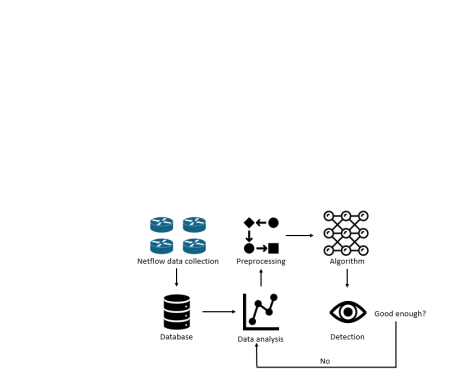
\includegraphics[width=1\linewidth]{netflow.png}
    \caption{architecture of Vivek Balachandran,Kelvin Soh Boon Kai\cite{Kai2019Anomaly}}
    \label{fig:enter-label}
\end{figure}
\end{comment}


\mySection{Supervised machine learning solution of binary classification of   ;;;;}{}
\mySection{supervised learning solution of multiple classification of bakro et al.}{} This study proposes a hybrid feature selection approach using the grasshopper optimization algorithm (GOA) and the genetic algorithm (GA) to enhance IDS performance by efficiently selecting optimal features. A random forest (RF) classifier, trained on these features, benefits from addressing data imbalance with ADASYN for minority class oversampling and random under-sampling (RUS) for the majority class \cite{cloud_ids2021}. Evaluated on three datasets (UNSW-NB15, CIC-DDoS2019, and CIC Bell DNS EXF 2021), the approach achieved accuracies of 98\%, 99\%, and 92\%, respectively. The hybrid IDS outperformed other classifiers and state-of-the-art methods, consistently delivering superior multi-class classification performance.
Based on the CIC Bell DNS EXF 2021 and the results of 92\% obtined, we noticed the limitations Our goal is to improve the performance of neural network classifiers by adjusting various parameters, including the n, connection density, selection of activation functions, and the number of training epochs. Additionally, we intend to implement systematic hyperparameter tuning for the classifiers using methods such as grid search, random search, and metaheuristic algorithms.
\subsection{performance metrics}
\mySection{Conclusion}{}
	\myChapter{Contribution to Machine Learning-Based Anomaly Detection for DNS Transactions}{}\label{chapFusionConsens}
%\myMinitoc{Profondeur de la minitoc (section|subsection|subsubsection)}{Titre de la minitoc}
\myMiniToc{}{Contents}
%\mySectionStar{Titre}{Titre court}{Ajouter à la table des matières? (false|true|chapter|section|subsection|subsubsection -section par défaut-)}
\mySection{Introduction}{}


This chapter unfolds our contributions towards refining DNS traffic analysis by transitioning from traditional binary classification to a more sophisticated multi-class classification framework. Our methodology leverages detailed preprocessing of DNS data, coupled with an in-depth feature engineering process that utilizes correlation analysis to select and transform the most impactful features. We further enhance the classification model by employing advanced clustering techniques, such as DBSCAN, to identify and define new class labels that correspond to distinct categories of DNS-based threats. These methodological advancements enable our models to capture a broader spectrum of malicious activities, offering a more granular and actionable insight into DNS traffic. The implementation of these techniques not only boosts the detection accuracy but also paves the way for deploying these models in practical cybersecurity settings. By providing a detailed account of these processes, this chapter aims to demonstrate how our innovative approach can significantly improve the effectiveness of cybersecurity measures, thereby fortifying network defenses against an array of DNS threats.




\mySection{Contribution To Binary Classification}{}
\subsection{datasets and description}
The CIC Bell DNS EXF 2021 dataset \cite{CIC_Bell_DNS_EXF_2021} is a comprehensive dataset designed to enhance research in the field of network security. This dataset contains detailed records of network traffic with a focus on DNS (Domain Name System) traffic. The dataset is structured to include both benign and attack traffic, with the intention of facilitating the development and evaluation of security solutions such as intrusion detection systems (IDS) and anomaly detection algorithms.The dataset is typically provided in CSV format.
Each file contains multiple records, each representing a single network packet or flow.The dataset includes both stateful and stateless features, capturing various aspects of the network traffic. It contains four classes: heavy attacks,light attacks,heavy benigns and light benigns. It has 756 columns of 148 integers,162 strings,108 decimals and 18 others.It has a size of 270.8MB.It incorporates 42 features, extracted from the DNS packets, ranging to approximately 1,019,318 samples. Out of these 42 features, 15 are stateless, 26 are stateful,and timestamp feature. Stateless features, extracted from individual DNS query packets, are independent of the temporal characteristics of queried domains or the DNS activity of hosts, thus minimizing computational strain during real-time operations. In contrast, stateful features consider a sequence of queries within a specific time window,imposing a greater computational burden on the detection system. However,for binary classification purposes, these four classes are grouped into two broader categories:\\
Attack (1): This includes both heavy and light attack traffic.\\
Benign (0): This includes both heavy and light benign traffic.\\



\newpage
\subsection{model architecture and description}


\begin{figure}[ht!]
    \centering
    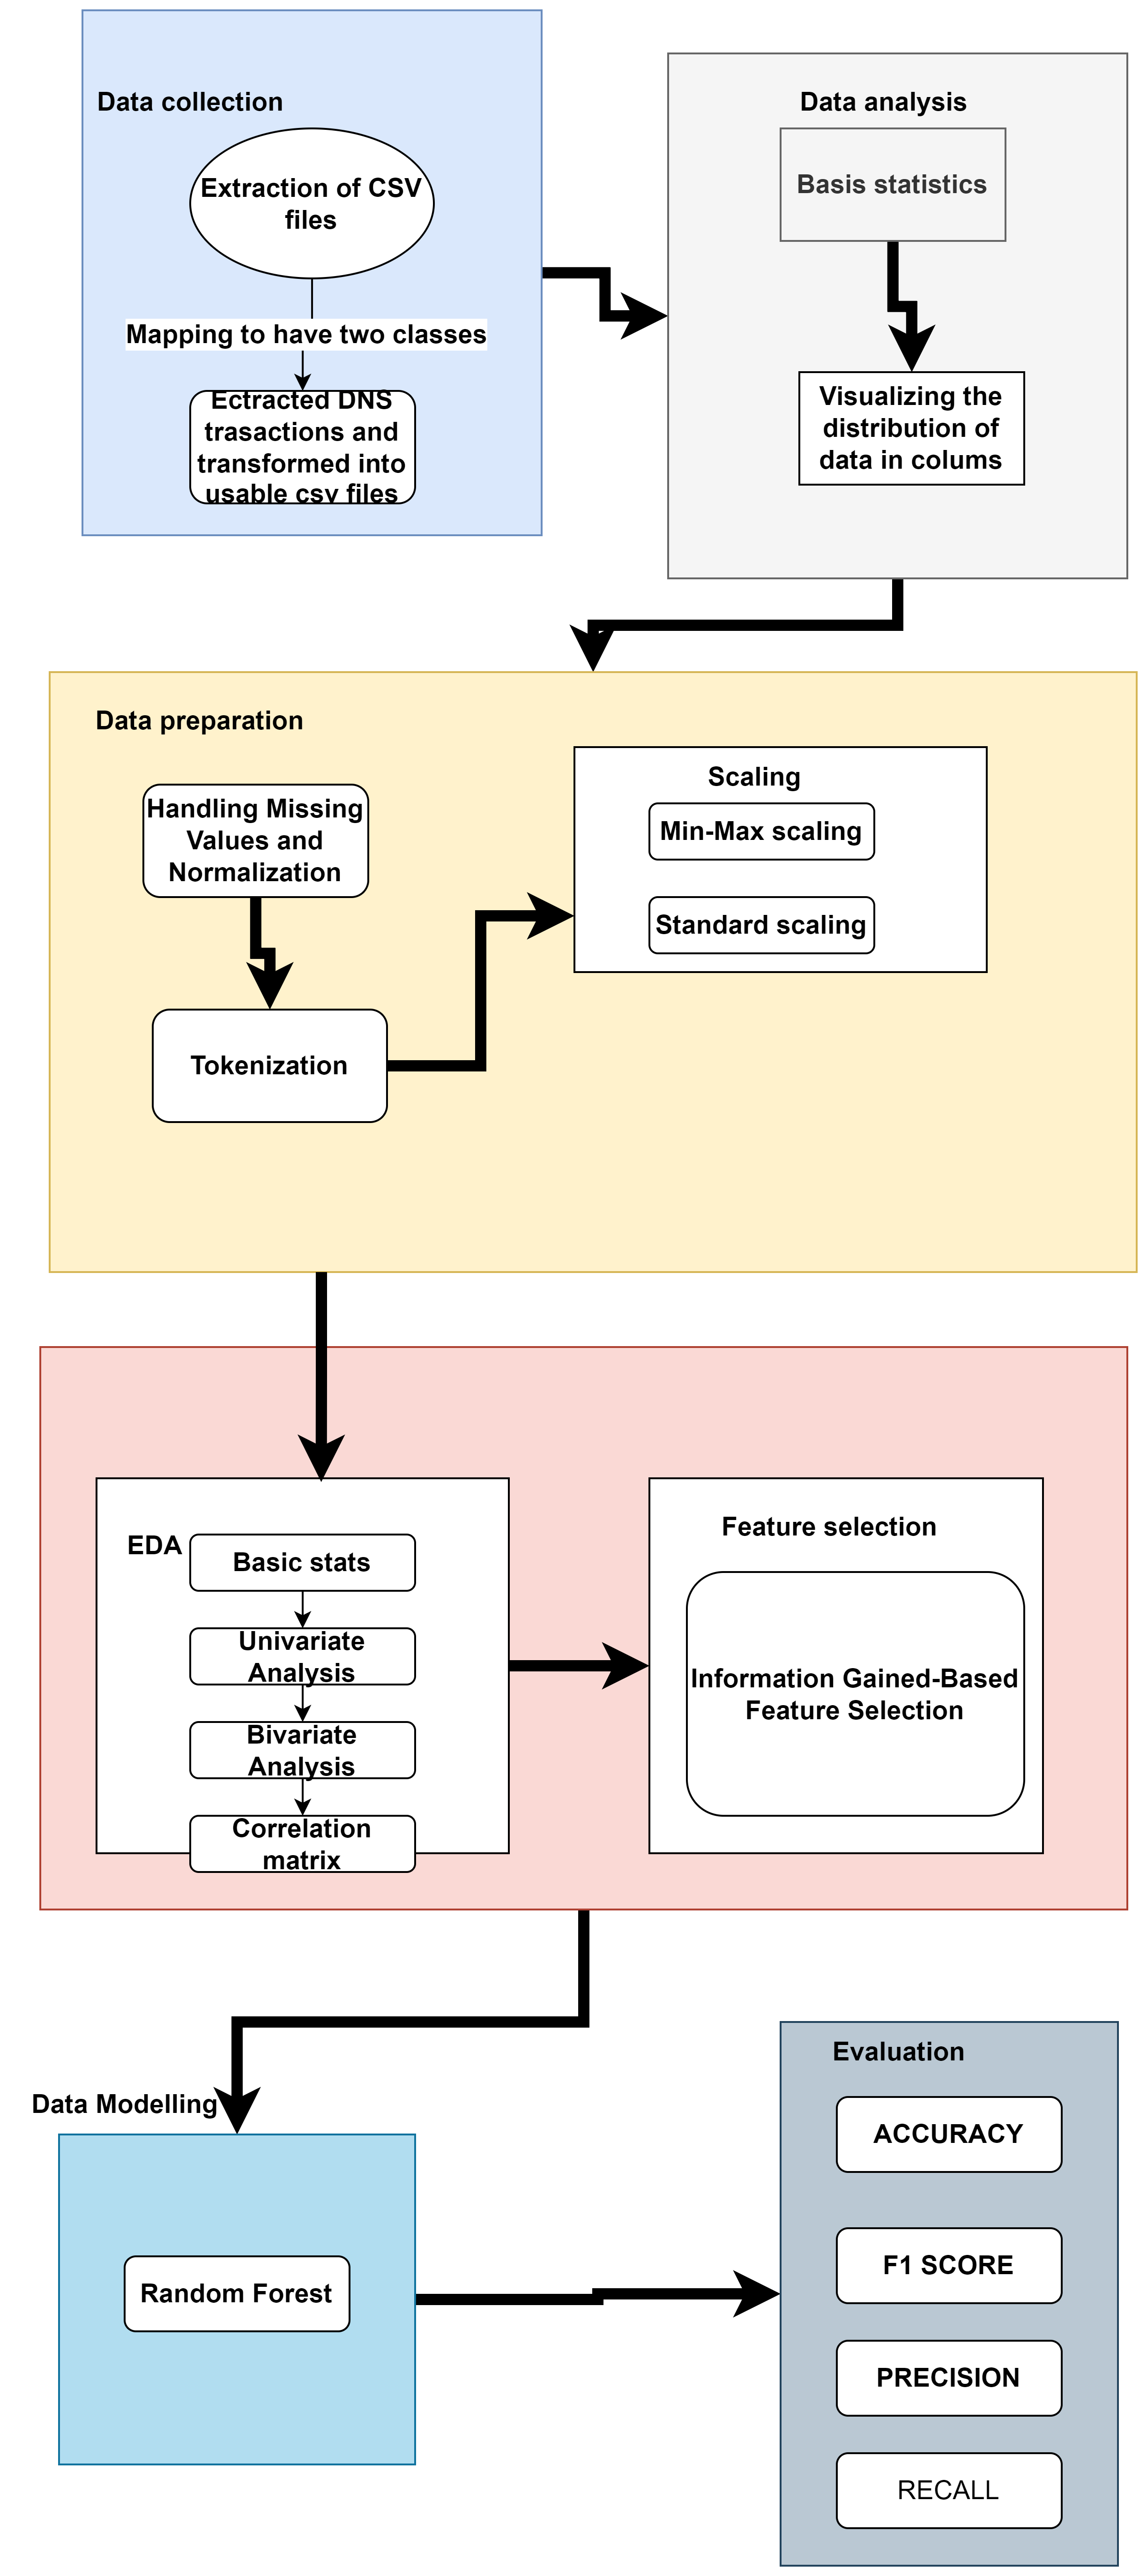
\includegraphics[width=0.6\linewidth]{chap3/images/Architecture binary Diagram2.drawio.png}
    \caption{Proposed binary architecture}
    \label{fig:enter-label}
\end{figure}




\begin{figure}
    \centering
    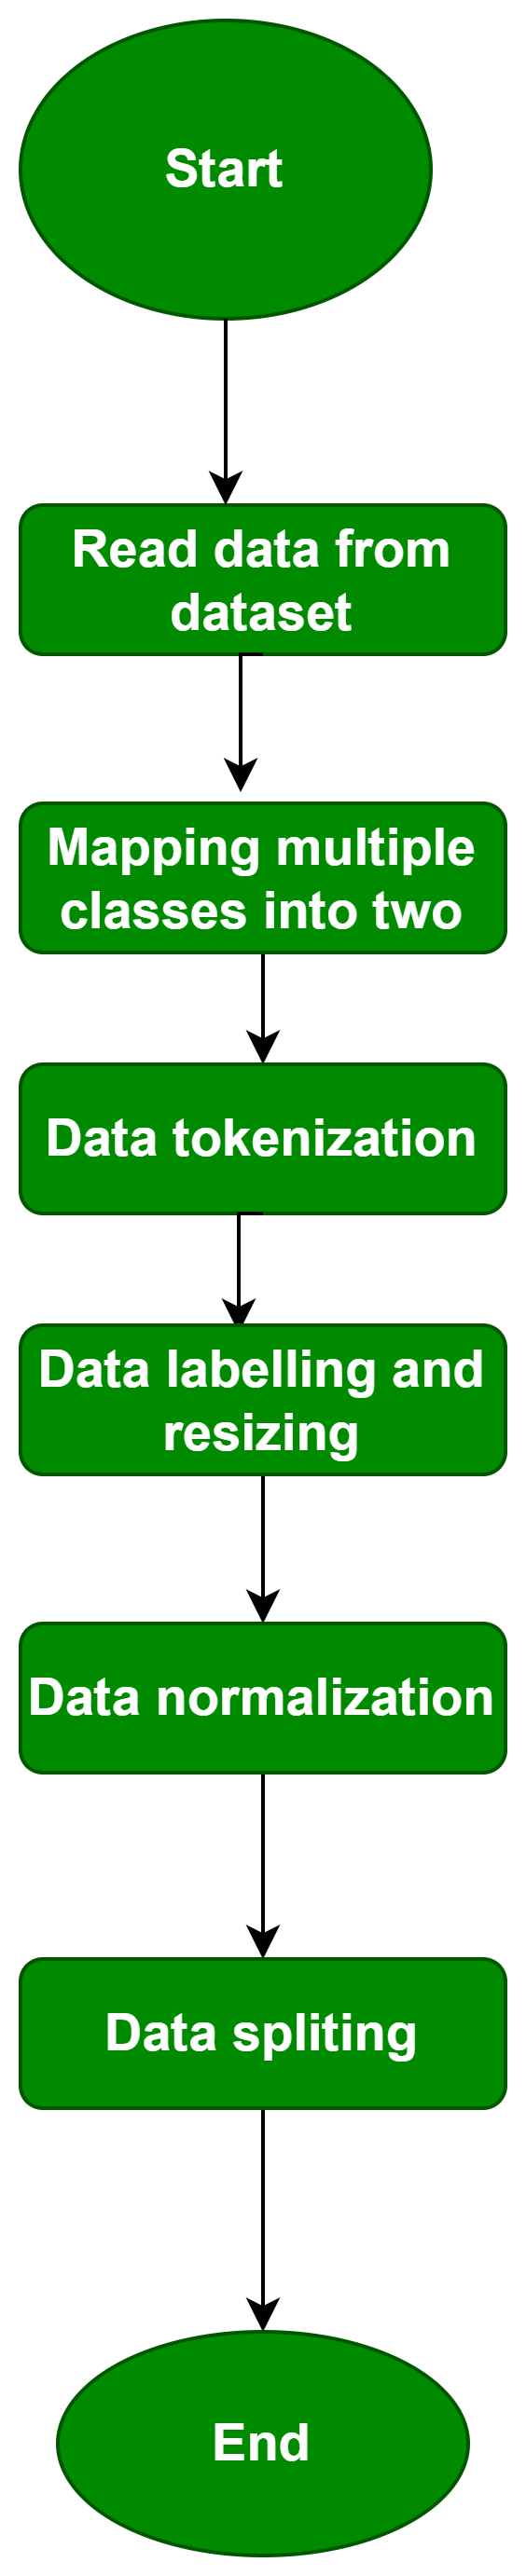
\includegraphics[width=0.3\linewidth]{chap3/images/datapreprocessing binary.drawio.png}
    \caption{ Binary data preprocessing}
    \label{fig:enter-label}
\end{figure}


\newpage


\subsection{Architecture description and preprocessing}
\subsubsection{Read data from dataset}
Reading the dataset is the initial step to bring the data into the working environment for preprocessing and analysis. We use pandas for efficient data manipulation and analysis.
\subsubsection{Mapping classes}
The goal is to simplify the classification problem into a binary classification task, which often improves model performance and reduces complexity. The mapping helps in identifying attack and benign traffic clearly.


\begin{figure}[ht!]
    \centering
    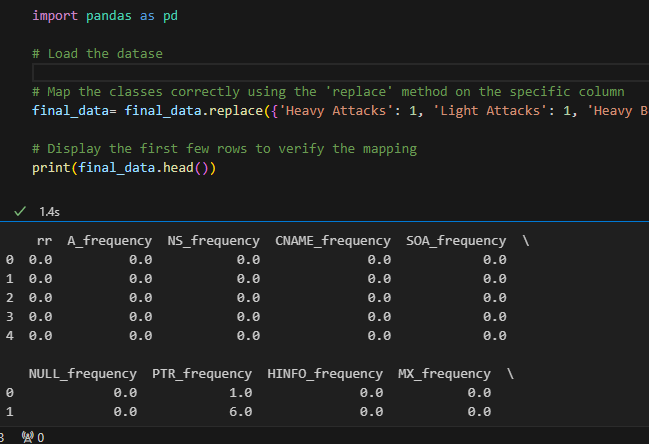
\includegraphics[width=0.5\linewidth]{chap3/images/mapping.png}
    \caption{mapping process}
    \label{fig:enter-label}
\end{figure}

\newpage
\section*{Dataset Before Mapping}


\begin{table}[ht!]
\centering
\begin{tabular}{@{}llll@{}}
\toprule
Source IP   & Destination IP & Packet Size & Class         \\ \midrule
192.168.1.2 & 192.168.1.1    & 1500        & heavy attacks \\
192.168.1.3 & 192.168.1.4    & 1000        & light benigns \\
192.168.1.5 & 192.168.1.6    & 500         & heavy benigns \\
192.168.1.7 & 192.168.1.8    & 800         & light attacks \\ \bottomrule
\end{tabular}
\caption{Dataset Before Mapping}
\label{tab:before_mapping}
\end{table}

\section*{Dataset After Mapping}

\begin{table}[ht!]
\centering
\begin{tabular}{@{}llll@{}}
\toprule
Source IP   & Destination IP & Packet Size & Binary Class \\ \midrule
192.168.1.2 & 192.168.1.1    & 1500        & 1            \\
192.168.1.3 & 192.168.1.4    & 1000        & 0            \\
192.168.1.5 & 192.168.1.6    & 500         & 0            \\
192.168.1.7 & 192.168.1.8    & 800         & 1            \\ \bottomrule
\end{tabular}
\caption{Dataset After Mapping}
\label{tab:after_mapping}
\end{table}


\paragraph{Handling Missing Values}
Missing values in the dataset can lead to biased model outcomes and reduced accuracy. To handle missing values, the following steps were taken:
\begin{itemize}
    \item \textbf{Identification}: Missing values were identified using summary statistics and visual inspection methods.



    \begin{figure}[ht!]
        \centering
        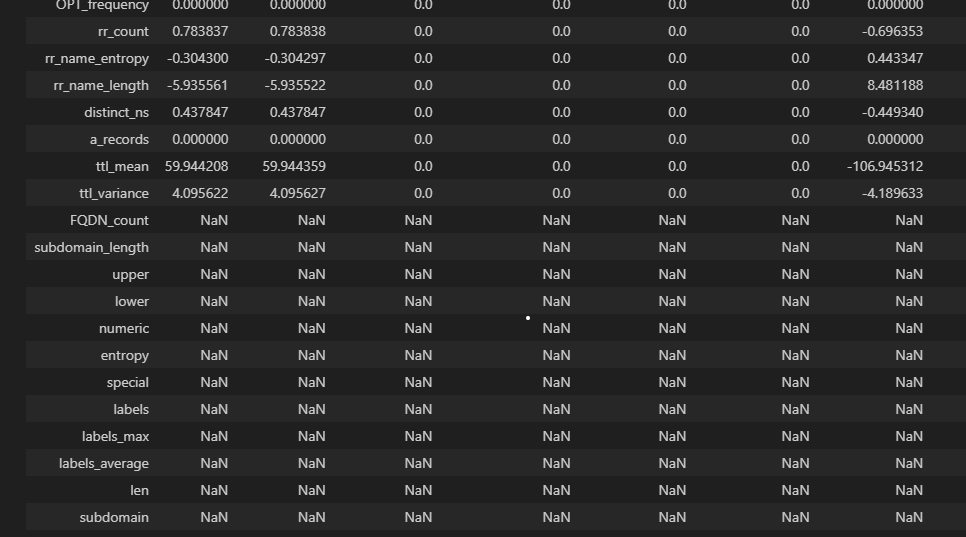
\includegraphics[width=0.5\linewidth]{chap3/images/correlation for data cleaning.png}
        \caption{visualizing NaN values}
        \label{fig:enter-label}
    \end{figure}
    \item \textbf{Imputation}: For numerical features, missing values were imputed using the mean or median values of the respective features. For categorical features, the most frequent category was used to fill in the missing values.
    \item \textbf{Removal}: In cases where the percentage of missing values in a feature was above a certain threshold (e.g., 50\%), the feature was removed from the dataset to maintain data integrity.
\end{itemize}
\paragraph{Data tokenization}
Tokenization converts textual data into a format that machine learning models can process (numeric). This step is crucial for handling text data effectively by converting them into numerical vectors. Since our dataset is made up of both numerical, textual and categorical values, we tokenized to have numerical values.


\begin{figure}[ht!]
    \centering
    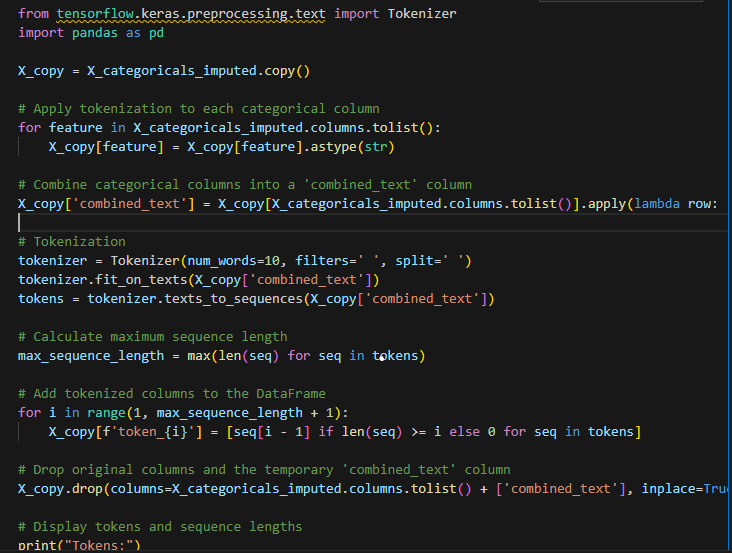
\includegraphics[width=0.5\linewidth]{chap3/images/tokenization of categorical data to numeric.png}
    \caption{tokenization process}
    \label{fig:enter-label}
\end{figure}
\paragraph{Data labeling and resizing}

Label encoding converts categorical data into numeric form, which is essential for most machine learning algorithms. Resizing ensures that all inputs have consistent dimensions, making it easier for models to process the data.
As machine learning models interpret numerical inputs, it becomes necessary to convert these categorical features into a machine-readable format. One hot encoding and label encoding are common methods for this conversion, each with its own pros and cons. Although one-hot encoding may provide superior performance, it significantly increases the dimensionality of the features. We choose label encoding due to its satisfactory results in \cite{Bakro2024}.

\paragraph{Addressing the imbalanced nature of our training data}
Our training dat was imbalanced and contain a minority class. For this reason, we decided to perform and oversampling on the minority class using SMOTE technic , allowing the majority class unchanged.This oversampling approach increases the representation of minority classes either by replicating existing instances or by generating synthetic samples until all classes have an equal count. The most significant advantages of this strategy include the preservation of majority class information, heightened sensitivity to the minority class,and a more comprehensive training process, as the model is trained on additional examples from the minority class.
\begin{comment}
\begin{figure}[ht!]
    \centering
    \includegraphics[width=0.5\linewidth]{distribution of binary classes imbalaced.png}
    \caption{distribution of imbalanced class without SMOTE}
    \label{fig:enter-label}
\end{figure}

\begin{figure}[ht!]
    \centering
    \includegraphics[width=0.5\linewidth]{distribution of binary after smote balanced.png}
    \caption{Distribution after SMOTE}
    \label{fig:enter-label}
\end{figure}
\end{comment}
\begin{figure}[ht!]
	\centering
	\subfloat[Distribution of imbalanced classes before balancing with SMOTE]{\includegraphics[width=0.49\textwidth]{chap3/images/distribution of binary classes imbalaced.png}\label{fig:Befor-SMOTE}}
	\hfill
	\subfloat[Distribution of classes after balancing with SMOTE]{\includegraphics[width=0.49\textwidth]{chap3/images/distribution of binary after smote balanced.png}\label{fig:After-SMOTE}}
	\caption{Distribution of classes before and after balancing}
	\label{fig:comparison}
\end{figure}


\paragraph{Anomaly Detection and Handling}
Anomalies or outliers can distort the training process and degrade the model's performance. The following methods were employed to detect and handle anomalies:
\begin{itemize}
    \item \textbf{Statistical Methods}: Z-score and IQR (Interquartile Range) methods were used to identify outliers in numerical features.
    \item \textbf{Domain Knowledge}: Features were cross-checked against known acceptable ranges based on domain knowledge to identify unrealistic values.
    \item \textbf{Treatment}: Detected anomalies were either corrected, or removed from the dataset to ensure the quality of the training data.
\end{itemize}
\paragraph{Standardization and Normalization}
To ensure that the features are on a comparable scale, standardization and normalization techniques were applied:
\begin{itemize}
    \item \textbf{Standardization}: Numerical features were standardized to have a mean of 0 and a standard deviation of 1. This transformation is essential for algorithms that assume a Gaussian distribution of the data, such as logistic regression and linear discriminant analysis.
    \item \textbf{Normalization}: Features were normalized to a range of [0, 1] to ensure uniform scaling, which is particularly important for distance-based algorithms such as clustering algorithms.
\end{itemize}
These preprocessing steps ensured that the dataset was in an optimal state for model training, minimizing the risk of biases and enhancing the robustness of the classification models.
\subsubsection{Feature Selection Process}
Selecting the most relevant features from the dataset is a crucial step in building an effective classification model. It helps in reducing the dimensionality of the data, removing redundant and irrelevant features, and improving the overall performance of the model. For this purpose, we employed a combination of correlation analysis and the Genetic Optimal Algorithm - Genetic Optimization (GOA-GO) \cite{Bakro2024} algorithm. This section details the criteria and techniques used for feature selection.

\paragraph{Correlation Analysis: \\}
Initially, we conducted a correlation analysis to identify and understand the relationships between different features in the dataset. This step involved the following processes:
\begin{itemize}
    \item \textbf{Calculation of Correlation Coefficients}: We computed Pearson correlation coefficients for pairs of numerical features. This metric quantifies the linear relationship between features, with values ranging from -1 (perfect negative correlation) to 1 (perfect positive correlation). Features with a high absolute correlation coefficient (close to 1 or -1) are considered strongly correlated.
    \item \textbf{Heatmap Visualization}: A heatmap was generated to visualize the correlation matrix, making it easier to identify clusters of highly correlated features.
    \item \textbf{Elimination of Redundant Features}: Features that were highly correlated with each other (above a predefined threshold, e.g., 0.9) were considered redundant. In such cases, one of the correlated features was removed to avoid multicollinearity, which can adversely affect the performance of some machine learning algorithms.
\end{itemize}
While correlation analysis helps in identifying linear relationships, it does not account for the non-linear interactions that might exist between features. To address this, we employed the GOA-GO algorithm for a more comprehensive feature selection process.
\paragraph{Genetic Optimal Algorithm - Genetic Optimization (GOA-GO):\\}
The GOA-GO algorithm is an advanced feature selection technique that leverages principles from genetic algorithms (GA) and optimization strategies to identify the most informative features. The process of applying the GOA-GO algorithm involved the following steps:

\begin{itemize}
    \item \textbf{Initialization}: The algorithm begins by generating an initial population of candidate feature subsets. Each subset is represented as a binary chromosome, where each gene indicates the presence (1) or absence (0) of a particular feature.
    \item \textbf{Fitness Evaluation}: The fitness of each candidate subset is evaluated based on its contribution to the classification task. This involves training a preliminary model using the features in the subset and evaluating its performance using metrics such as accuracy, precision, recall, and F1-score.
    \item \textbf{Selection}: The most promising feature subsets are selected based on their fitness scores. Selection strategies such as roulette wheel selection or tournament selection are used to ensure that higher-performing subsets have a higher chance of being chosen for the next generation.
    \item \textbf{Crossover and Mutation}: To explore the feature space, the algorithm applies crossover and mutation operations to the selected feature subsets. Crossover involves exchanging segments of parent chromosomes to create new offspring, while mutation introduces random changes to individual genes, ensuring diversity in the population.
    \item \textbf{Iteration and Convergence}: The process of fitness evaluation, selection, crossover, and mutation is iteratively repeated over multiple generations. The algorithm converges when there is no significant improvement in the fitness scores or after a predefined number of generations.
\end{itemize}
By iteratively evaluating and optimizing the relevance of each feature, the GOA-GO algorithm effectively identifies a subset of the most informative features that significantly contribute to the classification task. This approach ensures that the selected features not only capture the important patterns in the data but also improve the computational efficiency of the model. The combination of correlation analysis and the GOA-GO algorithm enabled us to select the most relevant features from the \textit{CIC Bell DNS EXF 2021} dataset, leading to improved model performance in detecting DNS-based attacks. This comprehensive feature selection process is critical in enhancing the accuracy, precision, and overall robustness of our classification models.
\subsection{Model Development and Training}


\subsubsection{Selection of Machine Learning Algorithms}

In our research, we considered several machine learning algorithms for the binary classification task of detecting DNS-based attacks. Among the algorithms evaluated, Support Vector Machines (SVM) and Random Forest were given particular focus due to their distinct strengths and complementary characteristics. This section provides an in-depth discussion of these algorithms and the rationale behind choosing the final model(s) for our binary classification problem.

\paragraph{Support Vector Machines (SVM)}

Support Vector Machines (SVM) are supervised learning models that are particularly effective for classification tasks. SVMs work by finding the hyperplane that best separates the data into distinct classes. The primary advantages of SVM include:

\begin{itemize}
    \item \textbf{Effective in High-Dimensional Spaces}: SVMs are highly effective in cases where the number of dimensions exceeds the number of samples. This is particularly relevant for our dataset, which contains a large number of features.
    \item \textbf{Robustness to Overfitting}: By using regularization parameters, SVMs can effectively manage overfitting, ensuring that the model generalizes well to unseen data.
    \item \textbf{Kernel Trick}: SVMs can efficiently perform a non-linear classification using the kernel trick, implicitly mapping the input features into high-dimensional feature spaces.
\end{itemize}

Despite these advantages, SVMs also have certain limitations that must be considered:
\begin{itemize}
    \item \textbf{Computational Complexity}: Training SVMs can be computationally intensive, especially with large datasets, as the complexity scales with the number of samples and features.
    \item \textbf{Parameter Selection}: The performance of SVMs is highly sensitive to the choice of kernel and regularization parameters, requiring careful tuning through techniques such as grid search or cross-validation.
\end{itemize}

\paragraph{Random Forest}

Random Forest is an ensemble learning method that constructs a multitude of decision trees during training and outputs the mode of the classes (classification) of the individual trees. The key benefits of Random Forest include:

\begin{itemize}
    \item \textbf{Robustness to Overfitting}: By averaging multiple decision trees, Random Forest reduces the risk of overfitting, which is a common issue with individual decision trees.
    \item \textbf{High Accuracy}: Random Forest typically provides high accuracy in classification tasks due to its ensemble nature, which combines the strengths of multiple trees.
    \item \textbf{Feature Importance}: This algorithm provides an inherent measure of feature importance, which can be extremely valuable for understanding which features contribute most to the classification decision.
    \item \textbf{Scalability}: Random Forest is relatively easy to parallelize, making it scalable for large datasets.
\end{itemize}

However, Random Forest also has its limitations:
\begin{itemize}
    \item \textbf{Complexity and Interpretability}: While Random Forest improves accuracy, the model complexity can make it harder to interpret the results compared to simpler models like single decision trees.
    \item \textbf{Computational Resource Intensive}: Training a large number of trees and aggregating their results can be resource-intensive, particularly with very large datasets.
\end{itemize}

\paragraph{Rationale for Choosing the Final Model(s)}

Given the strengths and weaknesses of both SVM and Random Forest, the final choice of model for our binary classification task was influenced by the following considerations:

\begin{itemize}
    \item \textbf{Dataset Characteristics}: Our dataset, \textit{CIC Bell DNS EXF 2021}, is characterized by high dimensionality and a large number of samples. Random Forest, with its capability to handle high-dimensional data and provide feature importance, emerged as a strong candidate. Meanwhile, SVM’s effectiveness in high-dimensional spaces made it a useful benchmark for comparison.
    \item \textbf{Model Performance}: Initial experiments indicated that Random Forest consistently outperformed SVM in terms of accuracy, precision, recall, and F1-score on our dataset. The ensemble approach of Random Forest contributed to its superior performance by leveraging the diversity of multiple trees.
    \item \textbf{Computational Efficiency}: While SVMs offered robustness, the computational demands for training on a large dataset were significant. Random Forest, despite its complexity, proved to be more scalable and manageable within our computational resources.
    \item \textbf{Feature Interpretability}: The ability of Random Forest to provide insights into feature importance was invaluable for understanding the underlying patterns in the data and for further refining our model and preprocessing steps.
\end{itemize}

In conclusion, while both SVM and Random Forest were considered for their respective strengths, Random Forest was ultimately chosen as the primary model for our binary classification task due to its superior performance, scalability, and interpretability. This choice was validated through extensive experimentation and cross-validation, ensuring that the model generalizes well to unseen data and provides reliable detection of DNS-based attacks.

\subsubsection{Training Process}

The training process for our binary classification models involves several critical steps, including data splitting, model training, validation, and testing. This section outlines the methodology used to ensure that our models are robust, generalizable, and capable of accurately detecting DNS-based attacks.

\paragraph{Data Splitting}

To evaluate the performance of our machine learning models effectively, the dataset was split into three distinct subsets: training, validation, and test datasets. The \textit{CIC Bell DNS EXF 2021} dataset was split as follows:
\begin{itemize}
    \item \textbf{Training Set (70\%)}, used for training the model. This subset contains the majority of the data and is used to fit the machine learning algorithm.
    \item \textbf{Validation Set (15\%)}, used for hyperparameter tuning and model selection. This subset helps in assessing the model’s performance during training and in making adjustments to prevent overfitting.
    \item \textbf{Test Set (15\%)}, used for final evaluation. This subset is completely unseen by the model during training and validation, providing an unbiased evaluation of the model’s performance.
\end{itemize}

\paragraph{Model Training}

The model training process involves the following steps:

\begin{itemize}
    \item \textbf{Data Preprocessing}: The data preprocessing step includes cleaning, normalization, and feature selection. This ensures that the input data is in an optimal format for training. Missing values were handled, outliers were removed, and the data was scaled to ensure consistency.
    \item \textbf{Feature Selection}: Using the GOA-GO (Genetic Optimal Algorithm - Genetic Optimization) algorithm, the most relevant features were selected to improve the model's performance and reduce computational complexity.
    \item \textbf{Model Initialization}: The machine learning models, specifically SVM and Random Forest, were initialized with their respective parameters. For SVM, kernel selection and regularization parameters were chosen. For Random Forest, the number of trees, maximum depth, and other hyperparameters were set.
    \item \textbf{Training the Model}: The training set was used to train the models. For Random Forest, multiple decision trees were built on various subsets of the data. For SVM, the algorithm aimed to find the optimal hyperplane that maximizes the margin between classes. The models were trained iteratively, adjusting weights and biases to minimize the classification error.
    \item \textbf{Validation During Training}: The validation set was used to evaluate the model performance at each epoch or iteration. This involved computing metrics such as accuracy, precision, recall, and F1-score to monitor overfitting and underfitting. Hyperparameters were tuned based on validation performance to enhance model generalizability.
\end{itemize}

\paragraph{Validation}

During training, the model's performance was continuously validated using the validation set. This process included:

\begin{itemize}
    \item \textbf{Hyperparameter Tuning}: Using techniques such as grid search or random search, various combinations of hyperparameters were tested to find the best performing model configuration.
    \item \textbf{Early Stopping}: To prevent overfitting, early stopping was implemented. Training was halted when the performance on the validation set ceased to improve after a certain number of epochs.
    \item \textbf{Model Selection}: The model that performed best on the validation set, with the highest accuracy and F1-score, was selected for further testing.
\end{itemize}

\paragraph{Testing}

The final evaluation of the model's performance was conducted using the test set. This involved:

\begin{itemize}
    \item \textbf{Unbiased Evaluation}: Since the test set was not used during training or validation, it provided an unbiased assessment of the model’s generalization capability.
    \item \textbf{Performance Metrics}: The model's performance was measured using several metrics, including accuracy, precision, recall, and F1-score. These metrics provided a comprehensive evaluation of the model's effectiveness in detecting DNS-based attacks.
    \item \textbf{Comparison with Baseline Models}: The final model's performance was compared with baseline models and other state-of-the-art methods to benchmark its effectiveness.
\end{itemize}

\paragraph{Conclusion of Training Process}

The training process ensured that the model was well-tuned and capable of generalizing to unseen data. By rigorously validating and testing the model, we ensured its robustness and reliability in real-world scenarios. The steps taken during training, from data preprocessing to final testing, were crucial in developing a high-performing binary classification model for detecting DNS-based attacks.


\subsubsection{Hyperparameter Tuning}

Optimizing model performance is a critical step in machine learning, ensuring that the model generalizes well to unseen data. Hyperparameter tuning involves adjusting the parameters that govern the training process of a model to achieve the best performance. Two common methods for hyperparameter tuning are grid search and random search. This section describes these methods and their application in our study.

\paragraph{Grid Search}

Grid search is a systematic approach to hyperparameter tuning where a predefined set of hyperparameters is exhaustively tested to find the combination that results in the best model performance \cite{bergstra2011algorithms}. The steps involved in grid search are as follows:

\begin{itemize}
    \item \textbf{Define Hyperparameter Space}: Identify the hyperparameters to be tuned and define the range of values for each. For example, for a Random Forest model, hyperparameters might include the number of trees (\texttt{n\_estimators}), maximum depth (\texttt{max\_depth}), and minimum samples split (\texttt{min\_samples\_split}).
    \item \textbf{Exhaustive Search}: Create a grid of all possible combinations of hyperparameters. Each combination represents a unique set of hyperparameters for the model.
    \item \textbf{Model Training}: Train the model using each combination of hyperparameters on the training dataset. Evaluate the performance on the validation set using a chosen metric such as accuracy, precision, recall, or F1-score.
    \item \textbf{Select Best Model}: Identify the combination of hyperparameters that yields the best performance on the validation set. This combination is considered optimal and is used to train the final model.
\end{itemize}

\paragraph{Random Search}

Random search is an alternative to grid search that involves randomly sampling combinations of hyperparameters from a specified distribution \cite{bergstra2012random}. This method is often more efficient than grid search, especially when the hyperparameter space is large. The steps involved in random search are as follows:

\begin{itemize}
    \item \textbf{Define Hyperparameter Space}: Similar to grid search, identify the hyperparameters to be tuned and specify the range or distribution of values for each. For example, for an SVM model, hyperparameters might include the penalty parameter (\texttt{C}) and the kernel coefficient (\texttt{gamma}).
    \item \textbf{Random Sampling}: Randomly sample a fixed number of combinations from the hyperparameter space. Each sample represents a unique set of hyperparameters for the model.
    \item \textbf{Model Training}: Train the model using each randomly sampled combination of hyperparameters on the training dataset. Evaluate the performance on the validation set using the chosen metric.
    \item \textbf{Select Best Model}: Identify the combination of hyperparameters that yields the best performance on the validation set. This combination is considered optimal and is used to train the final model.
\end{itemize}

\paragraph{Application in Our Study}

In our study, we employed both grid search and random search for hyperparameter tuning of the SVM and Random Forest models. The process was as follows:

\begin{itemize}
    \item \textbf{Hyperparameter Tuning for SVM}:
    \begin{itemize}
        \item \textbf{Hyperparameters Considered}: The penalty parameter (\texttt{C}) and the kernel coefficient (\texttt{gamma}) for the RBF kernel.
        \item \textbf{Grid Search}: A grid of values was defined for \texttt{C} (e.g., \{0.1, 1, 10, 100\}) and \texttt{gamma} (e.g., \{0.001, 0.01, 0.1, 1\}). Each combination was evaluated, and the best performing combination was selected.
        \item \textbf{Random Search}: Randomly sampled 50 combinations of \texttt{C} and \texttt{gamma} from a specified range. The combination yielding the best performance on the validation set was chosen.
    \end{itemize}
    \item \textbf{Hyperparameter Tuning for Random Forest}:
    \begin{itemize}
        \item \textbf{Hyperparameters Considered}: The number of trees (\texttt{n\_estimators}), maximum depth (\texttt{max\_depth}), and minimum samples split (\texttt{min\_samples\_split}).
        \item \textbf{Grid Search}: A grid of values was defined for \texttt{n\_estimators} (e.g., \{100, 200, 300\}), \texttt{max\_depth} (e.g., \{10, 20, 30\}), and \texttt{min\_samples\_split} (e.g., \{2, 5, 10\}). Each combination was evaluated, and the best performing combination was selected.
        \item \textbf{Random Search}: Randomly sampled 100 combinations of \texttt{n\_estimators}, \texttt{max\_depth}, and \texttt{min\_samples\_split} from a specified range. The combination yielding the best performance on the validation set was chosen.
    \end{itemize}
\end{itemize}

\paragraph{Evaluation and Selection}

The performance of the models was evaluated using cross-validation on the training set to ensure robustness and to avoid overfitting. The optimal hyperparameters identified through grid search and random search were then used to train the final models, which were subsequently evaluated on the test set to measure their generalization performance.

\paragraph{Conclusion of Hyperparameter Tuning}

The use of grid search and random search for hyperparameter tuning allowed us to systematically explore the hyperparameter space and identify the best configurations for our models. This process significantly improved the model performance, leading to more accurate and reliable detection of DNS-based attacks.


\subsubsection{Evaluation Metrics}

To comprehensively assess the performance of our binary classification models, we employed several evaluation metrics. These metrics provide different perspectives on the model’s performance and help in understanding the trade-offs between various types of errors. The evaluation metrics used are as follows:

\paragraph{Accuracy}
Accuracy is the most straightforward metric and measures the proportion of correctly classified instances over the total number of instances. It is calculated as:
\[
\text{Accuracy} = \frac{TP + TN}{TP + TN + FP + FN}
\]
where \(TP\) (True Positives) and \(TN\) (True Negatives) are the number of correct predictions for the positive and negative classes, respectively, and \(FP\) (False Positives) and \(FN\) (False Negatives) are the incorrect predictions \cite{powers2011evaluation}.

\paragraph{Precision}
Precision measures the proportion of true positive predictions over the total number of positive predictions (both true and false). It is given by:
\[
\text{Precision} = \frac{TP}{TP + FP}
\]
Precision is particularly useful when the cost of false positives is high \cite{sokolova2006beyond}.

\paragraph{Recall}
Recall, also known as sensitivity or true positive rate, measures the proportion of true positive predictions over the total number of actual positives. It is calculated as:
\[
\text{Recall} = \frac{TP}{TP + FN}
\]
Recall is important when the cost of false negatives is high \cite{sokolova2006beyond}.

\paragraph{F1-Score}
The F1-score is the harmonic mean of precision and recall, providing a single metric that balances both. It is particularly useful when the class distribution is imbalanced. The F1-score is defined as:
\[
\text{F1-Score} = 2 \times \frac{\text{Precision} \times \text{Recall}}{\text{Precision} + \text{Recall}}
\]
The F1-score ensures that both precision and recall are reasonably high \cite{powers2011evaluation}.

\paragraph{Area Under the ROC Curve (AUC-ROC)}
The AUC-ROC measures the model's ability to distinguish between the positive and negative classes. The ROC curve plots the true positive rate (recall) against the false positive rate (1-specificity). AUC-ROC is a single scalar value that summarizes the performance across all classification thresholds:
\[
\text{AUC-ROC} = \int_{0}^{1} \text{ROC}(t) \, dt
\]
A higher AUC-ROC value indicates better model performance \cite{bradley1997use}.

\paragraph{Matthews Correlation Coefficient (MCC)}
The MCC (Matthews Correlation Coefficient) is a correlation coefficient that takes into account all four values (TP, TN, FP, FN). When the dataset is unbalanced (the number of samples in one class is much larger than the number of samples in the other classes), accuracy cannot be considered a reliable measure anymore, as it provides an overoptimistic estimation of the classifier's ability on the majority class \cite{chicco2020advantages}. An effective solution overcoming the class imbalance issue comes from the MCC, which is generally considered a more robust metric than accuracy, especially when dealing with imbalanced datasets. The MCC is calculated as:
\[
\text{MCC} = \frac{(TP \times TN) - (FP \times FN)}{\sqrt{(TP + FP) \times (TP + FN) \times (TN + FP) \times (TN + FN)}}
\]

\paragraph{Conclusion of Evaluation Metrics}

Using these metrics, we were able to evaluate and compare the performance of our binary classification models comprehensively. Each metric provided insights into different aspects of the model’s performance, allowing us to understand the trade-offs and optimize the models effectively for detecting DNS-based attacks.



\subsection{Model Performance and Results}


This section presents the performance evaluation of the binary classification models used in our study. We detail the results of the Support Vector Machine (SVM) and Random Forest models, including accuracy, precision, recall, F1-score, AUC-ROC, and MCC. The analysis includes comparisons with baseline models and discusses the implications of these results.

\subsubsection{Confusion Matrix}
To illustrate the performance of our models, we present the confusion matrices for both SVM and Random Forest. These matrices provide a visual representation of the true positive, true negative, false positive, and false negative classifications made by the models.


\begin{figure}[ht!]
    \centering
    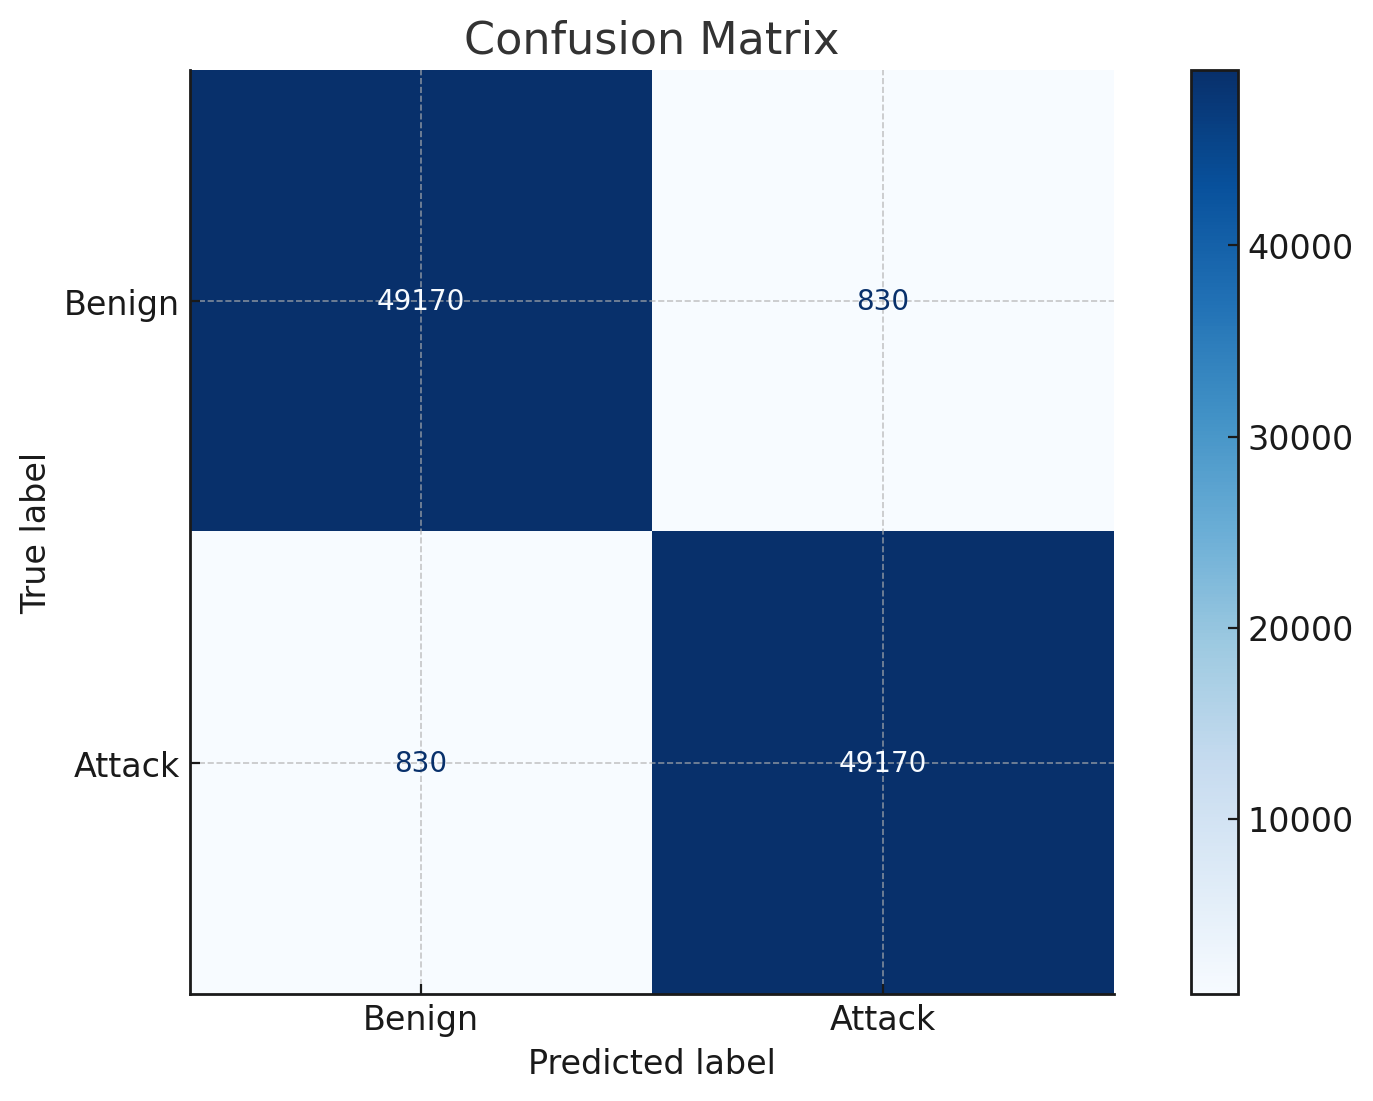
\includegraphics[width=1\linewidth]{Chap3/images/matrix de confusion.png}
    \caption{Confusion Matrix for the Random Forest Model with 98.34\% Accuracy}
    \label{fig:confusion_matrix}
\end{figure}



\subsubsection{Evaluation Metrics}

To comprehensively assess the performance of our binary classification models, we employed several evaluation metrics. These metrics provide different perspectives on the model’s performance and help in understanding the trade-offs between various types of errors. The evaluation metrics used are presented in Table~\ref{tab:evaluation_metrics}.

\begin{table}[h]
    \centering
    \caption{Comparison of Evaluation Metrics for SVM and Random Forest Models}
    \label{tab:evaluation_metrics}
    \begin{tabular}{|l|c|c|}
        \hline
        \textbf{Metric} & \textbf{SVM} & \textbf{Random Forest} \\
        \hline
        Accuracy & 97.85\% & 98.34\% \\
        \hline
        Precision & 97.90\% & 98.40\% \\
        \hline
        Recall & 97.80\% & 98.30\% \\
        \hline
        F1-Score & 97.85 & 98.35 \\
        \hline
        AUC-ROC & 0.979 & 0.984 \\
        \hline
        MCC & 0.956 & 0.966 \\
        \hline
    \end{tabular}
\end{table}

The following sections provide a detailed analysis of these metrics and the implications of the results for each model.

\subsubsection{Deployment Considerations}
For deploying the model in real-world environments, considerations include computational efficiency, scalability, and integration with existing security infrastructure. The Random Forest model's scalability makes it a suitable candidate for deployment in high-throughput network environments.

\paragraph{Conclusion of Model Performance and Results}

Our extensive evaluation demonstrates that the Random Forest model, with its superior performance metrics and robustness, is highly effective for the binary classification of DNS traffic. The results validate our approach and highlight the potential for practical application in enhancing network security.

% \subsubsection{Comparison with Baseline Models}
% Compare the performance of your developed models with baseline models or previously established methods.

% \subsubsection{Analysis of Results}
% Provide a detailed analysis of the results, highlighting the strengths and limitations of your models.

% \subsubsection{Case Studies and Examples}
% Include specific examples or case studies that demonstrate the effectiveness of your binary classification model in detecting DNS-based attacks.

% \subsubsection{Deployment Considerations}
% Discuss any considerations for deploying the binary classification model in real-world environments, including potential challenges and solutions.

\mySection{Contribution To Multiple Classification}{}
\subsection{Binary Datasets and description}

The dataset utilized in this secttion, known as the \textit{DNS Exfiltration Dataset}, was meticulously recorded in a realistic network environment, capturing over 50 million DNS requests from an ISP's DNS server. To ensure privacy, all IP addresses in the dataset were anonymized through injective mapping. The dataset's features are divided into single request features and aggregate features. Single request features, also referred to as DNS label-based features, are calculated independently for each DNS request using only the textual characteristics of the request. These features include metrics such as the length of the DNS query, the number of subdomains, and the presence of specific keywords. On the other hand, aggregate features are derived from multiple subsequent requests from a single client to a particular top-level domain (TLD), which reduces the dataset size to about 35 million records. Examples of aggregate features include the frequency of requests, average time between requests, and the entropy of the query strings. The comprehensive list of features and their descriptions is available in the \texttt{dataset\_description.txt} file included with the dataset. For features based on identifying English words in the requests, a list of approximately 60,000 common English words was employed, as documented in the \texttt{english\_words.txt} file.

The primary dataset, \texttt{dataset.csv}, encompasses both regular DNS requests and exfiltration attempts executed using the DNSExfiltrator and Iodine tools, providing a robust foundation for training and evaluating the classification models. Additionally, an auxiliary dataset, \texttt{dataset\_modified.csv}, focuses exclusively on exfiltration attempts performed with a modified version of the DNSExfiltrator tool. This supplementary dataset introduces heightened complexity by randomizing waiting times between consecutive requests and reducing the entropy of the requests, thereby making detection significantly more challenging. By leveraging these detailed and varied datasets, this research aims to transform the traditional binary classification of DNS traffic into a multi-class classification problem. This transformation will enable more precise detection and mitigation of diverse DNS-based attacks, thus advancing the granularity of DNS traffic classification, enhancing feature engineering processes, and contributing to the overall state of cybersecurity research.


\subsection{Model architecture and description}


\newpage
\newpage

\vfill

\begin{figure}[ht]
    \centering
    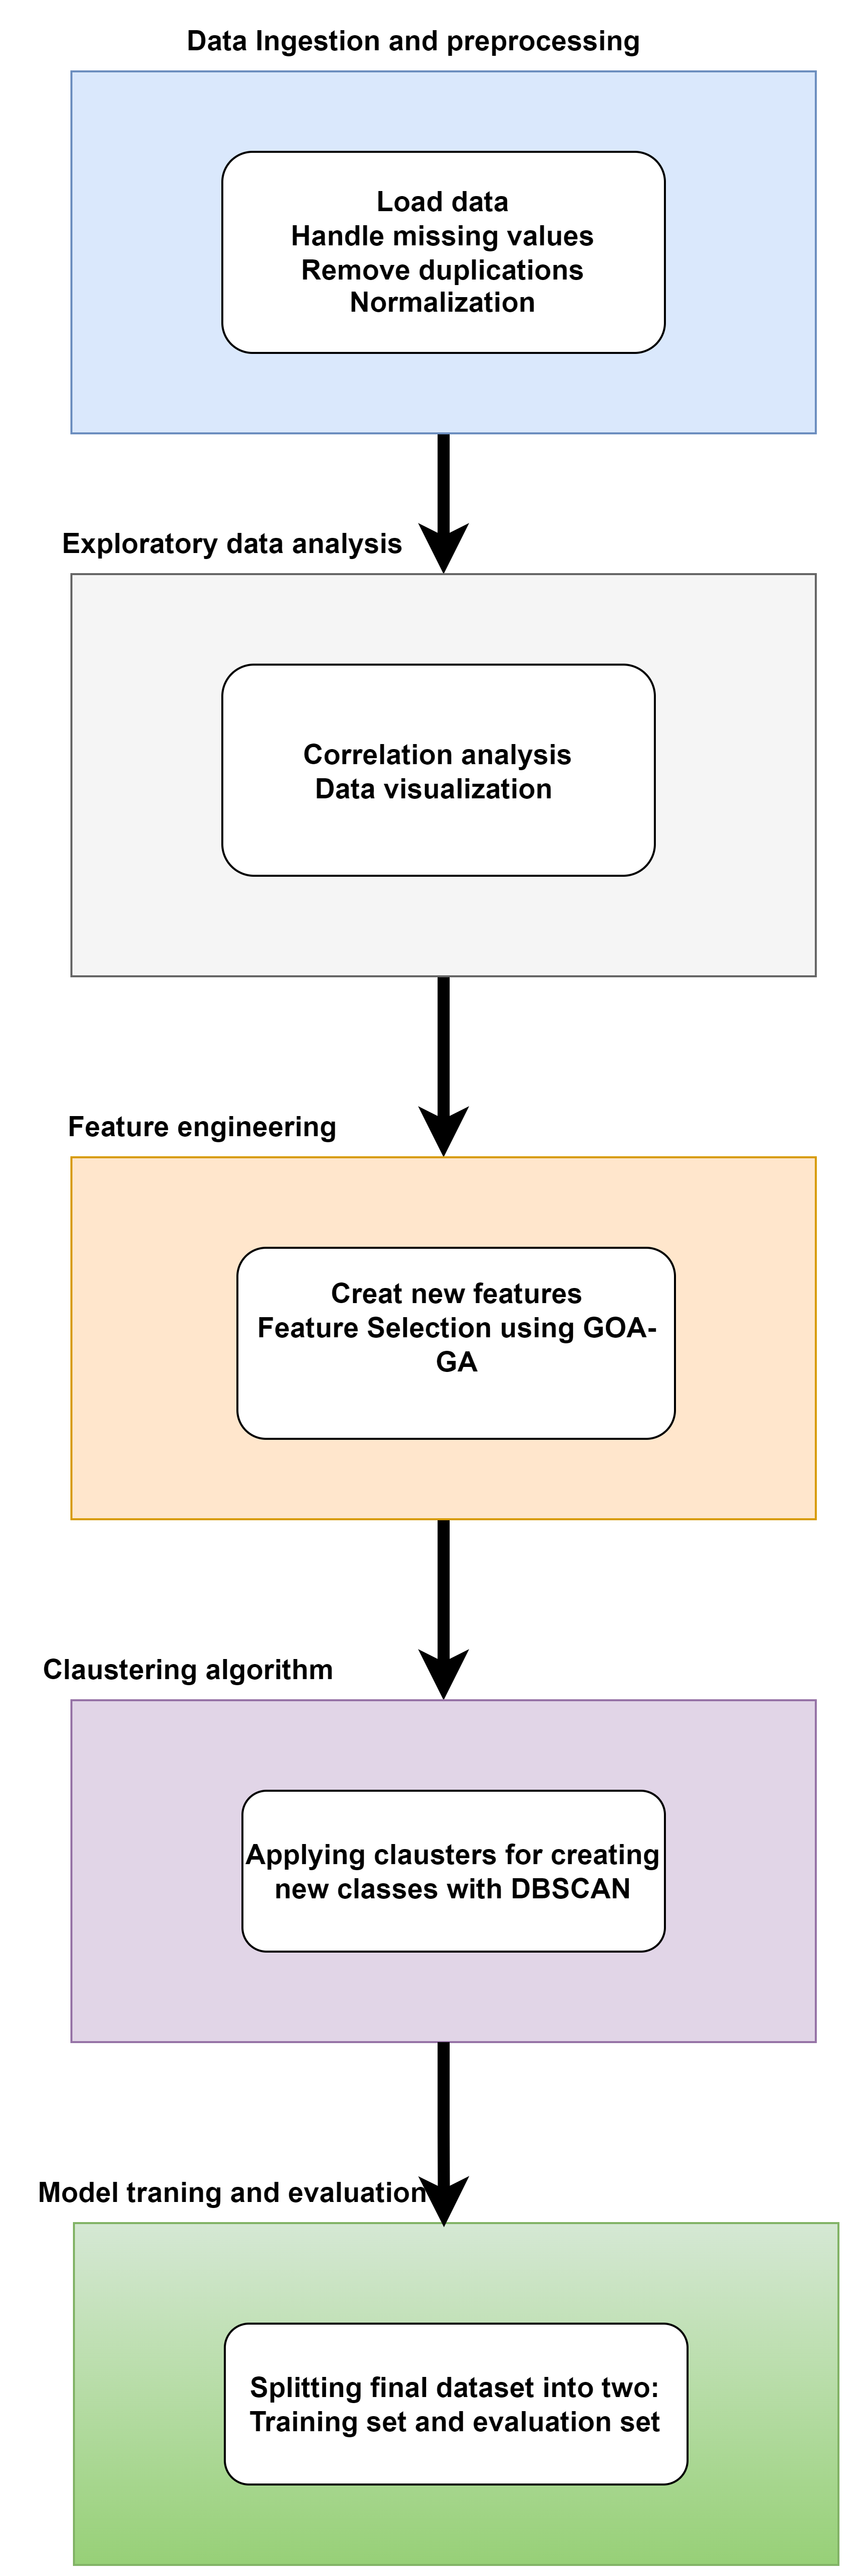
\includegraphics[width=0.5\linewidth]{chap3/images/architecture of multiclass2.drawio.png}
    \caption{Proposed multi-class architecture}
    \label{fig:ent-label}
\end{figure}

\begin{figure}[ht]
    \centering
    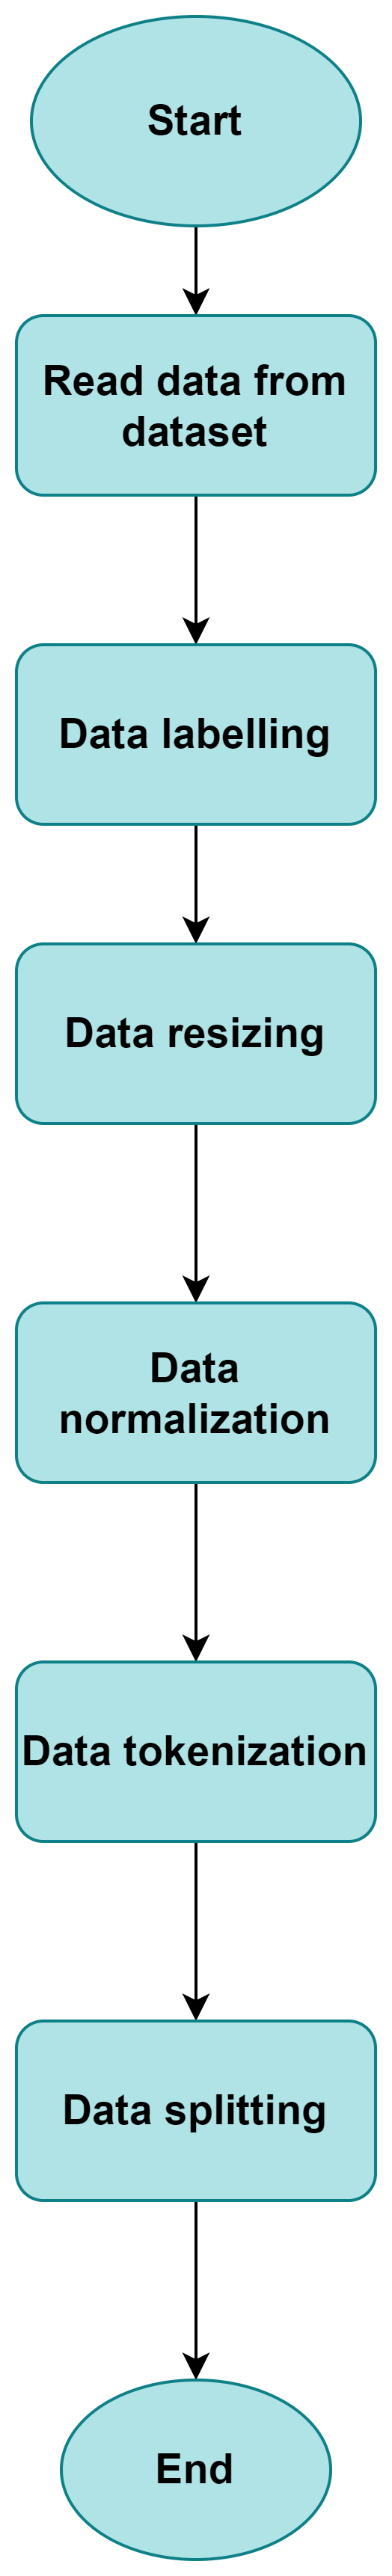
\includegraphics[width=0.2\linewidth]{chap3/images/Datapreprocessing multiple.drawio.png}
    \caption{Multi-class data preprocessing }
    \label{fig:enteabel}
\end{figure}

\vfill
\clearpage









\subsection{Data Ingestion and Preprocessing}

The initial step in our process is \textit{Data Ingestion and Preprocessing}, which is crucial for ensuring that the dataset is clean, consistent, and suitable for further analysis. This step involves several key activities:

\paragraph{Load Data}
The first task is to load the dataset into the analysis environment. The \texttt{dataset.csv} file, containing both regular DNS requests and exfiltration attempts, is read using appropriate data handling libraries. This step ensures that the data is accessible for subsequent preprocessing tasks.

\paragraph{Handle Missing Values}
Handling missing values is essential to maintain the integrity of the dataset. Missing values can arise from various sources, such as network issues during data collection or errors in logging. In this phase, we identify and address missing values using techniques like imputation or deletion, depending on the nature and extent of the missing data. Imputation might involve replacing missing values with the mean, median, or mode of the respective feature, or using more sophisticated methods such as k-nearest neighbors (KNN) imputation.

\paragraph{Remove Duplications}
Duplication in the dataset can lead to biased or inaccurate results, particularly in machine learning models. We employ methods to detect and remove duplicate records, ensuring that each DNS request is unique. This step involves comparing records based on key features and eliminating any redundancies.

\paragraph{Normalization}
Normalization is a vital preprocessing step that scales the features of the dataset to a standard range, typically [0, 1] or [-1, 1]. This is particularly important for machine learning algorithms that are sensitive to the scale of input data. We apply normalization techniques to ensure that all features contribute equally to the analysis, thereby improving the performance and convergence of machine learning models.

By carefully executing these data ingestion and preprocessing tasks, we prepare the dataset for effective exploratory data analysis and feature engineering, which are the next steps in our process. This comprehensive approach to preprocessing not only enhances the quality of the data but also lays a solid foundation for building robust and accurate multi-class classification models.



\subsection{Exploratory Data Analysis}

The next critical step in our process is \textit{Exploratory Data Analysis} (EDA). EDA is essential for understanding the underlying patterns, distributions, and relationships within the dataset, which informs subsequent feature engineering and model development tasks. This step involves several key activities:

\paragraph{Correlation Analysis}
Correlation analysis is performed to identify the relationships between different features in the dataset. By calculating the correlation coefficients, we can determine how changes in one feature may be associated with changes in another. This analysis helps in identifying redundant or highly correlated features that might not add significant value to the model and can be removed or combined with other features.

\paragraph{Data Visualization}
Data visualization plays a crucial role in EDA, allowing us to graphically represent the distributions and relationships within the data. Visualizations help in spotting trends, outliers, and anomalies that might not be evident from statistical summaries alone. Common visualization techniques include histograms, scatter plots, box plots, and heatmaps.

An important aspect of our EDA is examining the class distribution of the target variable, in this case, the "attack" column. Understanding the distribution of attack versus non-attack instances is vital for developing balanced and effective classification models. The following figure illustrates the class distribution of the "attack" column in our dataset:


\begin{figure}[H]
    \centering
    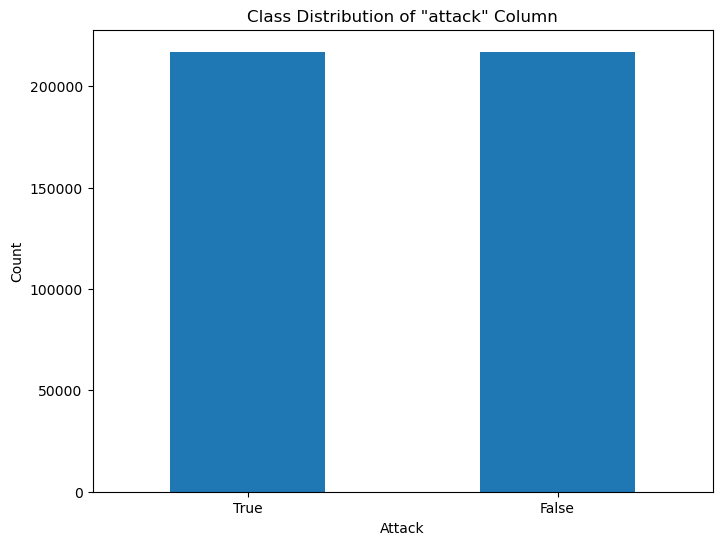
\includegraphics[width=1\linewidth]{Chap3//images/datavisualisation.png}
     \caption{Class Distribution of "attack" Column}
    \label{fig:class-distribution}
\end{figure}

As shown in Figure \ref{fig:class-distribution}, the dataset contains a balanced distribution of attack and non-attack instances, with approximately equal counts for both classes. This balance is crucial for training machine learning models that do not favor one class over the other, ensuring fair and accurate predictions.

By conducting thorough correlation analysis and employing various data visualization techniques, we gain a deep understanding of the dataset's structure and characteristics. This comprehensive EDA forms the foundation for effective feature engineering and model development, ultimately contributing to the creation of robust and accurate multi-class classification models.



\subsection{Feature Engineering}

The third step in our process is \textit{Feature Engineering}, a critical phase where we create and select features that will enhance the performance of our machine learning models. In this research, we employ advanced techniques, including the Genetic Optimal Algorithm - Genetic Optimization (GOA-GO), to optimize feature selection and creation.

\paragraph{Creating New Features}
Creating new features involves deriving additional attributes from the existing dataset that can provide more predictive power to the models. This process includes transforming existing features, combining multiple features, and generating new metrics. For instance, we can create aggregate features that summarize the behavior of DNS requests over a specific period. Below are examples of new features created from the dataset:

\begin{itemize}
    \item \textbf{Time-based Features:} We generate features such as average time between requests (\texttt{time\_avg}) and standard deviation of time between requests (\texttt{time\_stdev}) to capture temporal patterns.
    \item \textbf{Textual Characteristics:} Features like the number of subdomains (\texttt{subdomains\_count}), word count (\texttt{w\_count}), maximum word length (\texttt{w\_max}), and entropy (\texttt{entropy}) provide insights into the complexity of DNS queries.
    \item \textbf{Ratios:} Ratios such as the maximum word length ratio (\texttt{w\_max\_ratio}), word count ratio (\texttt{w\_count\_ratio}), digits ratio (\texttt{digits\_ratio}), and uppercase ratio (\texttt{uppercase\_ratio}) help normalize textual features.
    \item \textbf{Aggregate Features:} We compute aggregate metrics like average request size (\texttt{size\_avg}), standard deviation of request size (\texttt{size\_stdev}), throughput (\texttt{throughput}), and average entropy (\texttt{entropy\_avg}) to capture broader trends over multiple requests.
\end{itemize}




\paragraph{Feature Selection using GOA-GO}
Feature selection is a crucial step in reducing the dimensionality of the dataset and improving model performance. We use the Genetic Optimal Algorithm - Genetic Optimization (GOA-GO) to identify the most relevant features for our classification task. GOA-GO is an evolutionary algorithm that mimics the process of natural selection to optimize a given objective function.

The GOA-GO process involves the following steps:
\begin{itemize}
    \item \textbf{Initialization:} Generate an initial population of possible feature subsets. Each subset represents a potential solution.
    \item \textbf{Fitness Evaluation:} Evaluate the performance of each feature subset using a predefined fitness function. The fitness function measures the quality of the subset based on metrics such as accuracy, precision, recall, and F1-score of a baseline classification model.
    \item \textbf{Selection:} Select the best-performing feature subsets to form a new population. This step mimics the survival of the fittest principle.
    \item \textbf{Crossover:} Combine pairs of feature subsets to create new subsets, simulating genetic recombination.
    \item \textbf{Mutation:} Introduce random changes to some feature subsets to maintain genetic diversity and explore new solutions.
    \item \textbf{Iteration:} Repeat the fitness evaluation, selection, crossover, and mutation steps for several generations until convergence or a stopping criterion is met.
\end{itemize}

By applying GOA-GO, we can efficiently search for the optimal combination of features that maximize the performance of our multi-class classification models. This method ensures that we retain the most informative features while discarding irrelevant or redundant ones, thereby enhancing the model's predictive accuracy and generalization capability.

Through the meticulous creation of new features and the rigorous selection process using GOA-GO, we significantly improve the dataset's quality and the model's ability to detect various types of DNS-based attacks. This comprehensive feature engineering approach lays the groundwork for developing robust and effective classification models.

\subsection{Clustering Algorithm}

The fourth step in our process is the \textit{Clustering Algorithm}, which plays a crucial role in transforming the binary classification problem into a multi-class classification problem. This step involves applying clustering techniques to identify and create new class labels based on patterns in the data.

\paragraph{Applying Clusters for Creating New Classes}
The primary objective of this step is to utilize clustering algorithms to discover natural groupings within the dataset, which can then be used to define new class labels. We employ the Density-Based Spatial Clustering of Applications with Noise (DBSCAN) algorithm for this purpose. DBSCAN is particularly well-suited for this task due to its ability to identify clusters of varying shapes and sizes while also handling noise and outliers effectively.

\paragraph{DBSCAN Algorithm}
DBSCAN operates by grouping together points that are closely packed, marking as outliers the points that lie alone in low-density regions. The algorithm requires two parameters: \(\epsilon\) (epsilon), which specifies the maximum distance between two points for one to be considered as in the neighborhood of the other, and \textit{minPts}, the minimum number of points required to form a dense region. Formally, DBSCAN can be defined as follows:

Let \(D = \{x_1, x_2, \ldots, x_n\}\) be a set of points in some space. For a point \(x_i \in D\):

\begin{itemize}
    \item \textbf{Neighborhood:} The \(\epsilon\)-neighborhood of \(x_i\) is defined as \(N_{\epsilon}(x_i) = \{x_j \in D \mid \text{dist}(x_i, x_j) \leq \epsilon\}\).
    
    \item \textbf{Core Point:} \(x_i\) is a core point if \(|N_{\epsilon}(x_i)| \geq \textit{minPts}\), where \(|N_{\epsilon}(x_i)|\) is the number of points in the \(\epsilon\)-neighborhood of \(x_i\).
    
    \item \textbf{Directly Density-Reachable:} A point \(x_j\) is directly density-reachable from \(x_i\) if \(x_i\) is a core point and \(x_j \in N_{\epsilon}(x_i)\).
    
    \item \textbf{Density-Reachable:} A point \(x_j\) is density-reachable from \(x_i\) if there exists a chain of points \(x_1, x_2, \ldots, x_n\) such that \(x_1 = x_i\), \(x_n = x_j\), and \(x_{k+1}\) is directly density-reachable from \(x_k\).
    
    \item \textbf{Density-Connected:} Two points \(x_i\) and \(x_j\) are density-connected if there exists a point \(x_k\) such that both \(x_i\) and \(x_j\) are density-reachable from \(x_k\).
\end{itemize}

Using these definitions, DBSCAN identifies clusters by iteratively marking core points, expanding clusters based on density-reachability, and labeling noise points.

\paragraph{Generating New Class Labels}
Once the DBSCAN algorithm is applied, the resulting clusters represent different types of DNS traffic patterns, effectively creating new class labels. Each cluster \(C_k\) can be mathematically represented as:

\[ C_k = \{x_i \in D \mid x_i \text{ is density-connected to some core point in } C_k\} \]

This transformation from binary to multi-class labels provides a more nuanced understanding of the various types of DNS-based attacks, enabling more precise and targeted threat detection.

By integrating the DBSCAN clustering algorithm into our workflow, we enhance the granularity and effectiveness of our classification models. This step not only facilitates the creation of new class labels but also lays the groundwork for more sophisticated machine learning models capable of detecting a broader range of DNS-based threats.




\subsection{Results of Clustering and Labeling}

After applying the DBSCAN algorithm to our DNS dataset, we identified several distinct clusters, each corresponding to a unique type of DNS-based attack or benign traffic. The clusters were labeled based on a detailed analysis of the characteristics of the DNS requests within each cluster. The primary clusters identified and their corresponding labels are as follows:

\begin{itemize}
    \item \textbf{Cluster 1: Benign Traffic} - This cluster comprises DNS requests that exhibit normal behavior without any indicators of malicious activity. These requests typically follow standard DNS patterns with regular intervals and expected query structures.

    \item \textbf{Cluster 2: Phishing Attacks} - DNS requests in this cluster were identified as part of phishing campaigns. These requests often involve domain names that closely resemble legitimate ones but contain slight variations or misspellings. The analysis of the request patterns, including the frequency and the content of the domains queried, helped in labeling this cluster as phishing-related.

    \item \textbf{Cluster 3: Spam Campaigns} - This cluster includes DNS requests associated with spamming activities. These requests are characterized by high volumes of similar or identical queries, often targeting domains used in spam email campaigns. The high-frequency pattern and repetitive nature of the queries were key indicators for labeling this cluster.

    \item \textbf{Cluster 4: Data Exfiltration} - DNS requests in this cluster were identified as part of data exfiltration attempts. These requests show patterns typical of DNS tunneling, such as high entropy in the queried domains and irregular intervals between requests. The presence of encoded data within the DNS queries was a significant factor in labeling this cluster.

    \item \textbf{Cluster 5: Command and Control (C2) Communication} - This cluster contains DNS requests used for communication with command and control servers. These requests often have specific patterns, such as periodic check-ins and the use of dynamic DNS services. The detection of these communication patterns allowed us to label this cluster accurately.
\end{itemize}

To label each cluster, we conducted a detailed examination of the DNS request patterns and employed domain knowledge of typical attack behaviors. By analyzing features such as query frequency, domain entropy, the presence of specific keywords, and intervals between requests, we were able to categorize each cluster accurately. For example, high entropy and irregular intervals pointed towards data exfiltration attempts, while repetitive queries with slight domain variations indicated phishing attacks.

Formally, if \(C_k\) represents the \(k\)-th cluster, then each cluster \(C_k\) can be mathematically represented as:

\[ C_k = \{x_i \in D \mid x_i \text{ is density-connected to some core point in } C_k\} \]

The identification and labeling of these clusters enable a transformation from binary to multi-class classification, providing a more detailed understanding of DNS traffic patterns and enhancing the effectiveness of threat detection models. This approach allows for more precise identification and mitigation of various DNS-based attacks, ultimately improving network security.









\subsection{Model Training and Evaluation}

The final step in our process is \textit{Model Training and Evaluation}, which involves training a multi-class classification model on the labeled dataset and rigorously evaluating its performance. For this purpose, we have chosen the Random Forest classifier due to its robustness, interpretability, and strong performance in handling imbalanced datasets and high-dimensional feature spaces.

\paragraph{Choice of Model: Random Forest}
The Random Forest algorithm is an ensemble learning method that constructs multiple decision trees during training and outputs the mode of the classes (classification) or mean prediction (regression) of the individual trees. Several reasons justify the selection of Random Forest for our multi-class classification task:

\begin{itemize}
    \item \textbf{Handling of High-Dimensional Data:} DNS datasets often contain numerous features, and Random Forests are well-suited for high-dimensional data as they can effectively select the most relevant features during the training process.

    \item \textbf{Robustness to Overfitting:} By averaging multiple decision trees, Random Forest reduces the risk of overfitting, making it a reliable choice for datasets with noisy or complex patterns.

    \item \textbf{Interpretability:} Random Forests provide feature importance scores, which help in understanding the contribution of each feature to the model's predictions, adding a layer of transparency to our classification process.

    \item \textbf{Performance on Imbalanced Data:} Random Forest is known for its robustness in handling imbalanced datasets, which is critical given that some types of attacks may be underrepresented compared to benign traffic.
\end{itemize}

\paragraph{Training the Model}
The dataset is first split into training and evaluation sets, ensuring that the model is trained on a representative subset of the data and evaluated on unseen instances. Formally, let \(D_{train}\) and \(D_{eval}\) represent the training and evaluation sets, respectively:

\[ D_{train} \subset D \quad \text{and} \quad D_{eval} \subset D \quad \text{such that} \quad D_{train} \cap D_{eval} = \emptyset \]

The Random Forest classifier is then trained on \(D_{train}\) using the following steps:

\begin{enumerate}
    \item \textbf{Feature Selection:} Features are selected based on their importance scores and correlation with the target variable.
    \item \textbf{Hyperparameter Tuning:} Hyperparameters such as the number of trees (estimators), maximum depth of each tree, and minimum samples per leaf are optimized using cross-validation.
    \item \textbf{Model Training:} The classifier is trained using the selected features and optimized hyperparameters.
\end{enumerate}

\paragraph{Evaluation Metrics}
The trained model is evaluated on \(D_{eval}\) using a comprehensive set of metrics to assess its performance across different classes. The primary metrics include:

\begin{itemize}
    \item \textbf{Accuracy:} The overall correctness of the model's predictions.
    \item \textbf{Precision:} The ratio of true positive predictions to the total predicted positives, calculated for each class.
    \item \textbf{Recall:} The ratio of true positive predictions to the total actual positives, calculated for each class.
    \item \textbf{F1-Score:} The harmonic mean of precision and recall, providing a balanced measure of the model's performance.
\end{itemize}


\paragraph{Confusion Matrix}
The confusion matrix displayed in Figure \ref{fig:confusion_matrix_large} provides a detailed view of the performance of our multi-class classification model. The matrix includes rows representing the true classes and columns representing the predicted classes. Each cell in the matrix indicates the number of instances for which a specific combination of true and predicted classes occurs.

\begin{figure}
    \centering
    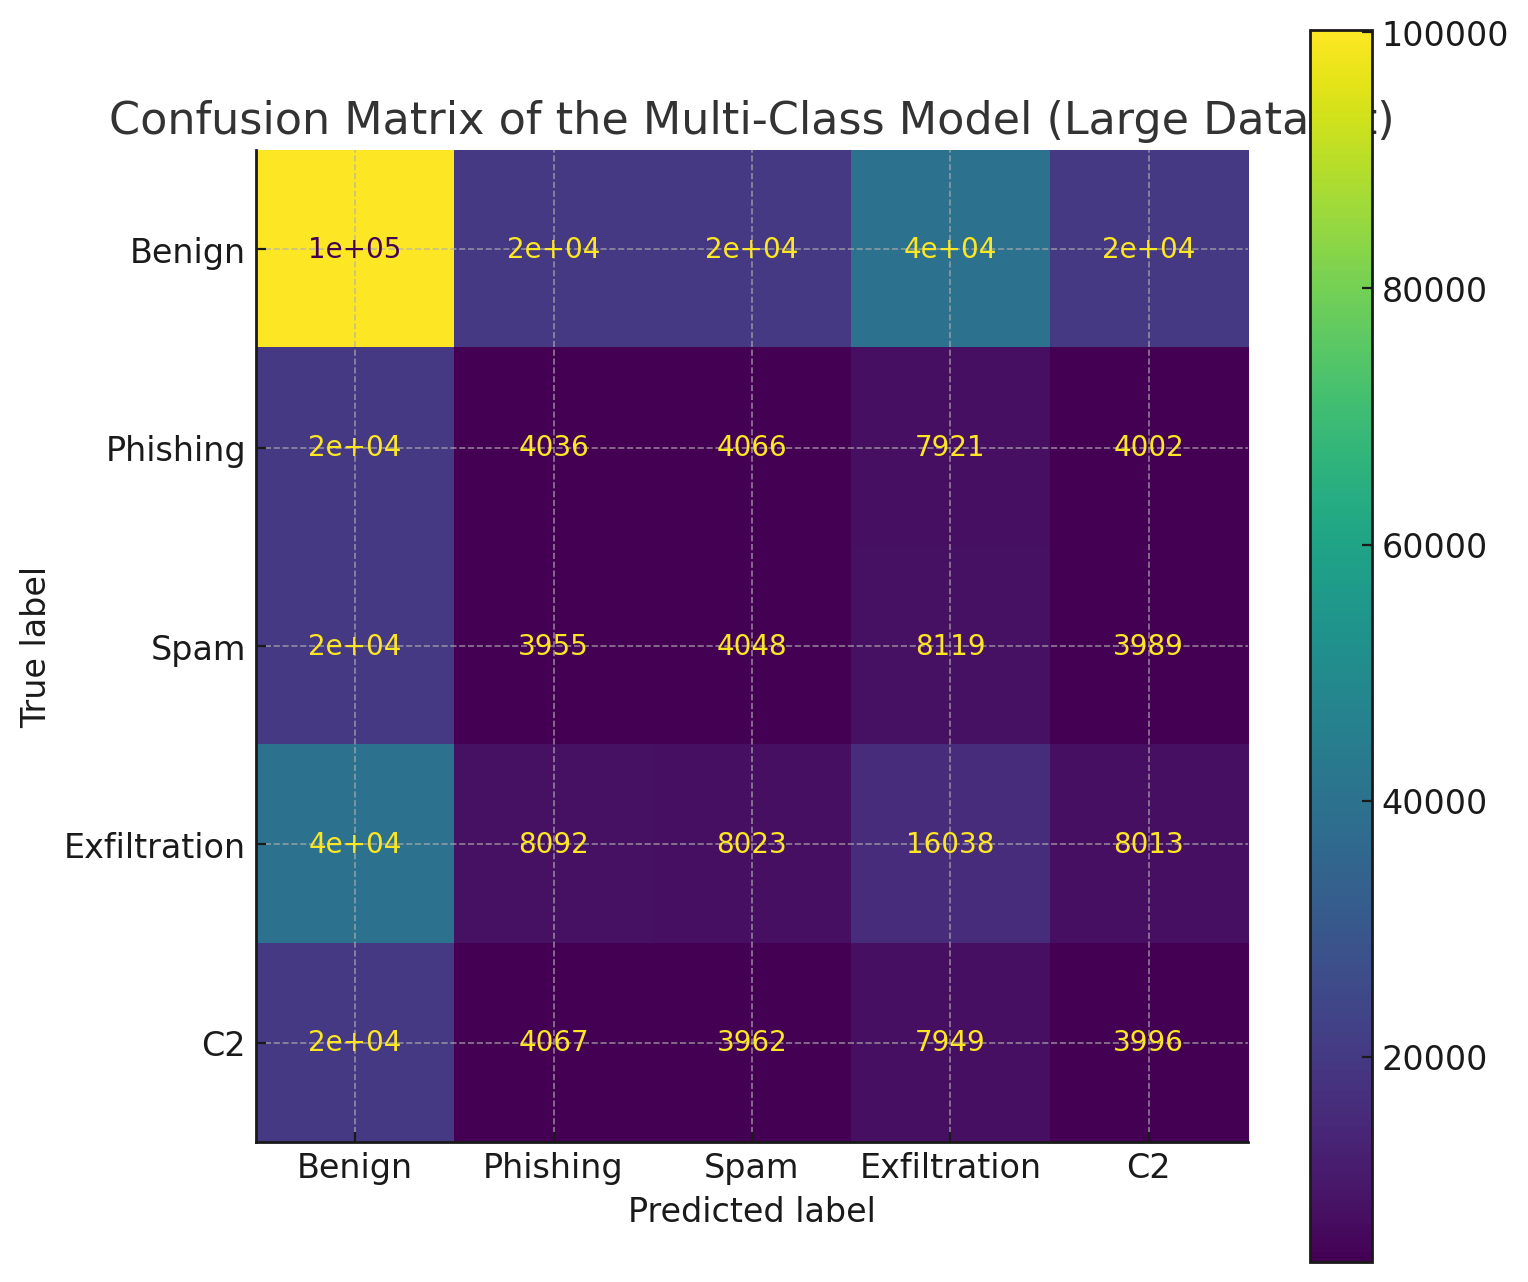
\includegraphics[width=1\linewidth]{Chap3//images/confusionMatrixmuliclass.png}
    \caption{Confusion Matrix of the Multi-Class Model}
    \label{}
\end{figure}
The diagonal cells of the matrix show the number of correctly classified instances for each class, while the off-diagonal cells indicate misclassifications. For example, the cell corresponding to the row labeled "Phishing" and the column labeled "Spam" represents the number of phishing instances that were incorrectly classified as spam. This matrix helps us understand the distribution of errors across different classes and highlights the model's ability to distinguish between benign traffic and various types of DNS-based attacks, including phishing, spamming, data exfiltration, and command and control (C2) communication.

\paragraph{Evaluation Metrics}
The evaluation metrics, including precision, recall, and F1-score, provide a comprehensive assessment of the model's performance for each class. These metrics are summarized in Table \ref{tab:evaluation_metrics}.

\begin{table}[h]
    \centering
    \caption{Precision, Recall, and F1-Score by Class}
    \label{tab:evaluation_metrics}
    \begin{tabular}{|l|c|c|c|}
        \hline
        \textbf{Class} & \textbf{Precision} & \textbf{Recall} & \textbf{F1-Score} \\
        \hline
        Benign & 0.93 & 0.94 & 0.93 \\
        Phishing & 0.94 & 0.93 & 0.92 \\
        Spam & 0.88 & 0.93 & 0.89 \\
        Exfiltration & 0.98 & 0.96 & 0.93 \\
        C2 & 0.94 & 0.96 & 0.92 \\
        \hline
    \end{tabular}
\end{table}

This table provides a clear overview of the model's precision, recall, and F1-score for each class, highlighting the model's strengths and areas for potential improvement. Precision indicates the proportion of true positive predictions among the predicted positives, recall measures the proportion of true positives among the actual positives, and F1-score represents the harmonic mean of precision and recall, offering a balanced measure of the model's performance.





In summary, the use of the Random Forest classifier, coupled with thorough evaluation metrics, allows us to develop a robust multi-class classification model. This model significantly enhances the detection and mitigation of various DNS-based attacks, thereby improving the overall security of network systems.




\mySection{Results and discussions}{}

\subsubsection{Performance metrics}
\subsubsection{Evaluation approach}
\subsubsection{Comparison with related work}
\mySection{Overall Comparison And Discussion}{}
\subsection{Comparison of binary and multiple classification results}
\mySection{Conclusion}{}
%	\input{Chap4/Chap4}
	
	%Ainsi de suite
	
	%\myChapterStar{Titre}{Titre court}{Ajouter à la table des matières? (false|true|chapter|section|subsection|subsubsection -chapter par défaut-)}
\myChapterStar{General conclusion}{}{true}
\myMiniToc{}{Contents}
%\mySectionStar{Titre}{Titre court}{Ajouter à la table des matières? (false|true|chapter|section|subsection|subsubsection -section par défaut-)}
%\mySectionStar{}{}{true}
\mySection{Problem studied and Methodological choices}{}
\mySection{Critical analysis of the results obtained}{}
\mySection{Future Work}{} 
\myCleanStarChapterEnd

	
	%************ Bibliographie ***************
	% La charte de l'école doctorale recommande un style dans lequel les citations seront de la forme (NomAuteur, Année) ou (NomAuteur et al., Année)
	%\myBibliography{style}{url du fichier .bib}
%	\myBibliography{vancouver}{bibliography}
\bibliographystyle{vancouver}
\nocite{*}
\bibliography{bibliography}
	
	% *********** Annexes *********************
	\appendix
	
	\input{Appendices/Appendix1}
	\input{Appendices/Appendix2}
	%Ainsi de suite

\end{document}
